\documentclass[11pt,twoside]{report}

%%%%%%%%%%%%%%%%%%%%%%%%%%%%%%%%%%%%%%%%%%%%%%%%%%%%%%%%%%%%%%%%%%%%%%%%%%%%%

% Definitions for the title page
% Edit these to provide the correct information
% e.g. \newcommand{\reportauthor}{Timothy Kimber}

\newcommand{\reporttitle}{Hazard Detection for Cyclists}
\newcommand{\reportauthor}{Peter Hedley}
\newcommand{\supervisor}{Dr Stefan Leutenegger}
\newcommand{\degreetype}{Computing}

%%%%%%%%%%%%%%%%%%%%%%%%%%%%%%%%%%%%%%%%%%%%%%%%%%%%%%%%%%%%%%%%%%%%%%%%%%%%%

% load some definitions and default packages
%%%%%%%%%%%%%%%%%%%%%%%%%%%%%%%%%%%%%%%%%
% University Assignment Title Page 
% LaTeX Template
% Version 1.0 (27/12/12)
%
% This template has been downloaded from:
% http://www.LaTeXTemplates.com
%
% Original author:
% WikiBooks (http://en.wikibooks.org/wiki/LaTeX/Title_Creation)
%
% License:
% CC BY-NC-SA 3.0 (http://creativecommons.org/licenses/by-nc-sa/3.0/)
% 
%
%%%%%%%%%%%%%%%%%%%%%%%%%%%%%%%%%%%%%%%%%
%----------------------------------------------------------------------------------------
%	PACKAGES AND OTHER DOCUMENT CONFIGURATIONS
%----------------------------------------------------------------------------------------
\usepackage[a4paper,hmargin=2.8cm,vmargin=2.0cm,includeheadfoot]{geometry}
\usepackage{textpos}
%\usepackage{natbib} % for bibliography
\usepackage{tabularx,longtable,multirow,subfigure,caption}%hangcaption
\usepackage{fncylab} %formatting of labels
\usepackage{fancyhdr} % page layout
\usepackage{url} % URLs
\usepackage[english]{babel}
\usepackage{amsmath}
\usepackage{graphicx}
\usepackage{dsfont}
\usepackage{epstopdf} % automatically replace .eps with .pdf in graphics
\usepackage{backref} % needed for citations
\usepackage{array}
\usepackage{latexsym}
\usepackage[pdftex,pagebackref,hypertexnames=false,colorlinks]{hyperref} % provide links in pdf

\hypersetup{pdftitle={},
  pdfsubject={}, 
  pdfauthor={},
  pdfkeywords={}, 
  pdfstartview=FitH,
  pdfpagemode={UseOutlines},% None, FullScreen, UseOutlines
  bookmarksnumbered=true, bookmarksopen=true, colorlinks,
    citecolor=black,%
    filecolor=black,%
    linkcolor=black,%
    urlcolor=black}

\usepackage[all]{hypcap}


%\usepackage{color}
%\usepackage[tight,ugly]{units}
%\usepackage{float}
%\usepackage{tcolorbox}
%\usepackage[colorinlistoftodos]{todonotes}
% \usepackage{ntheorem}
% \theoremstyle{break}
% \newtheorem{lemma}{Lemma}
% \newtheorem{theorem}{Theorem}
% \newtheorem{remark}{Remark}
% \newtheorem{definition}{Definition}
% \newtheorem{proof}{Proof}


%%% Default fonts
\renewcommand*{\rmdefault}{bch}
\renewcommand*{\ttdefault}{cmtt}



%%% Default settings (page layout)
\setlength{\parindent}{0em}  % indentation of paragraph

\setlength{\headheight}{14.5pt}
\pagestyle{fancy}
\renewcommand{\chaptermark}[1]{\markboth{\chaptername\ \thechapter.\ #1}{}} 

\fancyfoot[ER,OL]{\sffamily\textbf{\thepage}}%Page no. in the left on odd pages and on right on even pages
\fancyfoot[OC,EC]{\sffamily }
\renewcommand{\headrulewidth}{0.1pt}
\renewcommand{\footrulewidth}{0.1pt}
\captionsetup{margin=10pt,font=small,labelfont=bf}


%--- chapter heading

\def\@makechapterhead#1{%
  \vspace*{10\p@}%
  {\parindent \z@ \raggedright \sffamily
    \interlinepenalty\@M
    \Huge\bfseries \thechapter \space\space #1\par\nobreak
    \vskip 30\p@
  }}

%---chapter heading for \chapter*  
\def\@makeschapterhead#1{%
  \vspace*{10\p@}%
  {\parindent \z@ \raggedright
    \sffamily
    \interlinepenalty\@M
    \Huge \bfseries  #1\par\nobreak
    \vskip 30\p@
  }}

\allowdisplaybreaks


% load some macros
% Here, you can define your own macros. Some examples are given below.

\newcommand{\R}[0]{\mathds{R}} % real numbers
\newcommand{\Z}[0]{\mathds{Z}} % integers
\newcommand{\N}[0]{\mathds{N}} % natural numbers
\newcommand{\C}[0]{\mathds{C}} % complex numbers
\renewcommand{\vec}[1]{{\boldsymbol{{#1}}}} % vector
\newcommand{\mat}[1]{{\boldsymbol{{#1}}}} % matrix



\usepackage{amsmath}
\usepackage{textcomp}
\usepackage{enumitem}
\usepackage{graphicx}
\usepackage{tabularx}
\usepackage{amsfonts}
\usepackage{float}
\usepackage{wrapfig}
\usepackage[table]{xcolor}
\usepackage{amssymb}
\usepackage{longtable}
\usepackage[section]{placeins}
\usepackage[]{setspace}
\usepackage[ruled]{algorithm2e}
\newcommand\mycommfont[1]{\footnotesize\ttfamily\textcolor{gray}{#1}}
\SetCommentSty{mycommfont}

\date{September 2015}


\begin{document}

% load title page
% Last modification: 2015-08-17 (Marc Deisenroth)
\begin{titlepage}

\newcommand{\HRule}{\rule{\linewidth}{0.5mm}} % Defines a new command for the horizontal lines, change thickness here


%----------------------------------------------------------------------------------------
%	LOGO SECTION
%----------------------------------------------------------------------------------------


\includegraphics[width = 4cm]{./figures/imperial}\\[0.5cm] 

\center % Center remainder of the page

%----------------------------------------------------------------------------------------
%	HEADING SECTIONS
%----------------------------------------------------------------------------------------

\textsc{\Large Imperial College London}\\[0.5cm] 
\textsc{\large Department of Computing}\\[0.5cm] 

%----------------------------------------------------------------------------------------
%	TITLE SECTION
%----------------------------------------------------------------------------------------

\HRule \\[0.4cm]
{ \huge \bfseries \reporttitle}\\ % Title of your document
\HRule \\[1.5cm]
 
%----------------------------------------------------------------------------------------
%	AUTHOR SECTION
%----------------------------------------------------------------------------------------

\begin{minipage}{0.4\textwidth}
\begin{flushleft} \large
\emph{Author:}\\
\reportauthor % Your name
\end{flushleft}
\end{minipage}
~
\begin{minipage}{0.4\textwidth}
\begin{flushright} \large
\emph{Supervisor:} \\
\supervisor % Supervisor's Name
\end{flushright}
\end{minipage}\\[4cm]


%----------------------------------------------------------------------------------------
%	FOOTER & DATE SECTION
%----------------------------------------------------------------------------------------
\vfill % Fill the rest of the page with whitespace
Submitted in partial fulfillment of the requirements for the MSc degree in
\degreetype~of Imperial College London\\[0.5cm]

\makeatletter
\@date 
\makeatother


\end{titlepage}



% page numbering etc.
\pagenumbering{roman}
\clearpage{\pagestyle{empty}\cleardoublepage}
\setcounter{page}{1}
\pagestyle{fancy}

%%%%%%%%%%%%%%%%%%%%%%%%%%%%%%%%%%%%
\begin{abstract}
Recently in the news, and as any London cyclist has experienced, there are numerous potentially fatal hazards on a morning commute. Cars turn directly in front of you, doors often open unexpectedly and pedestrians amble into the road taking a selfie. The project is aimed at detecting potential hazards through the use of an on-board camera, and alerting the cyclist and pedestrian/car to it. The problem requires computer vision techniques and SLAM algorithms for spacial understanding.
\newline \newline
This project investigates state-of-the-art methods in image segmentation, object tracking, and develops a novel architecture for cyclist path prediction. The results of which, although not realtime provide a solid foundation for future research in the area and suggests potential modifications to the system for that to become a reality.
\end{abstract}

\cleardoublepage
%%%%%%%%%%%%%%%%%%%%%%%%%%%%%%%%%%%%
\section*{Acknowledgments}
Many thanks to my supervisor Dr Stefan Leutenegger for his continued support throughout the process. As a student with less than a year of computer science experience this project would not have been possible without him.
\newline \newline
Also thanks to the other students on my course who have helped with ideas about how the project should progress.

\clearpage{\pagestyle{empty}\cleardoublepage}

%%%%%%%%%%%%%%%%%%%%%%%%%%%%%%%%%%%%
%--- table of contents
\fancyhead[RE,LO]{\sffamily {Table of Contents}}
\tableofcontents 


\clearpage{\pagestyle{empty}\cleardoublepage}
\pagenumbering{arabic}
\setcounter{page}{1}
\fancyhead[LE,RO]{\slshape \rightmark}
\fancyhead[LO,RE]{\slshape \leftmark}

%%%%%%%%%%%%%%%%%%%%%%%%%%%%%%%%%%%%

%TODO check that dimensions are right!!
\chapter{Introduction}

%%%%%%%%%%%%%%%%%%%%%%%%%%%%%%%%%%%%
There were c. 18,500 cycling accidents and 3,500 deaths on British roads in 2016 \cite{DFT_fig}. Of these accidents 80\% occur during the day and driver/rider error accounts for 71\% of the total collisions \cite{DFT_fig2}. The most common place for a cycling incident is at a road junction with 75\% of collisions occurring there \cite{DFT_fig3}. With cycling becoming a more accepted form of transport, the need to protect and modify bikes with a comprehensive safety system is important.

\subsection{Road Map} The report develops a system for collision detection and is split into two main sections, object detection and understanding the 3D environment. The sections are developed simultaneously throughout the report and are discussed within the following chapters.

\paragraph{Background} This chapter discusses the current research into the area of instance segmentation, recurrent networks, optimisation and SLAM. It first describes recent advances in computer vision relevant to the current state-of-the-art method Mask RCNN. Mask RCNN combines a number of advances in different fields, namely image classification, detection and segmentation. The chapter then continues with discussion around recurrent networks for path prediction, and methods of optimising these networks. Finally a brief discussion on SLAM and object tracking which are both highly active and voluminous fields of research in their own right.

\paragraph{Contribution}
The contribution chapter discusses depth approximations when there is a depth camera failure, object tracking and prediction. In particular it discusses combining various tracking methods into a comprehensive system that both combines the advantages of the respective algorithms and mitigates their potential weaknesses. Once the ability to track objects is discussed, models for prediction of future locations are developed. This leads to a novel recurrent network to predict future bicycle locations from image, and pose data gathered from previous frames. Finally a method of combining these predictive models, and determining whether a collision is likely to occur is discussed in the latter part of the chapter. These sections all talk through the various modules required in the system which is described below in Figure \ref{software_soln1}


\noindent \begin{figure}[h!]
	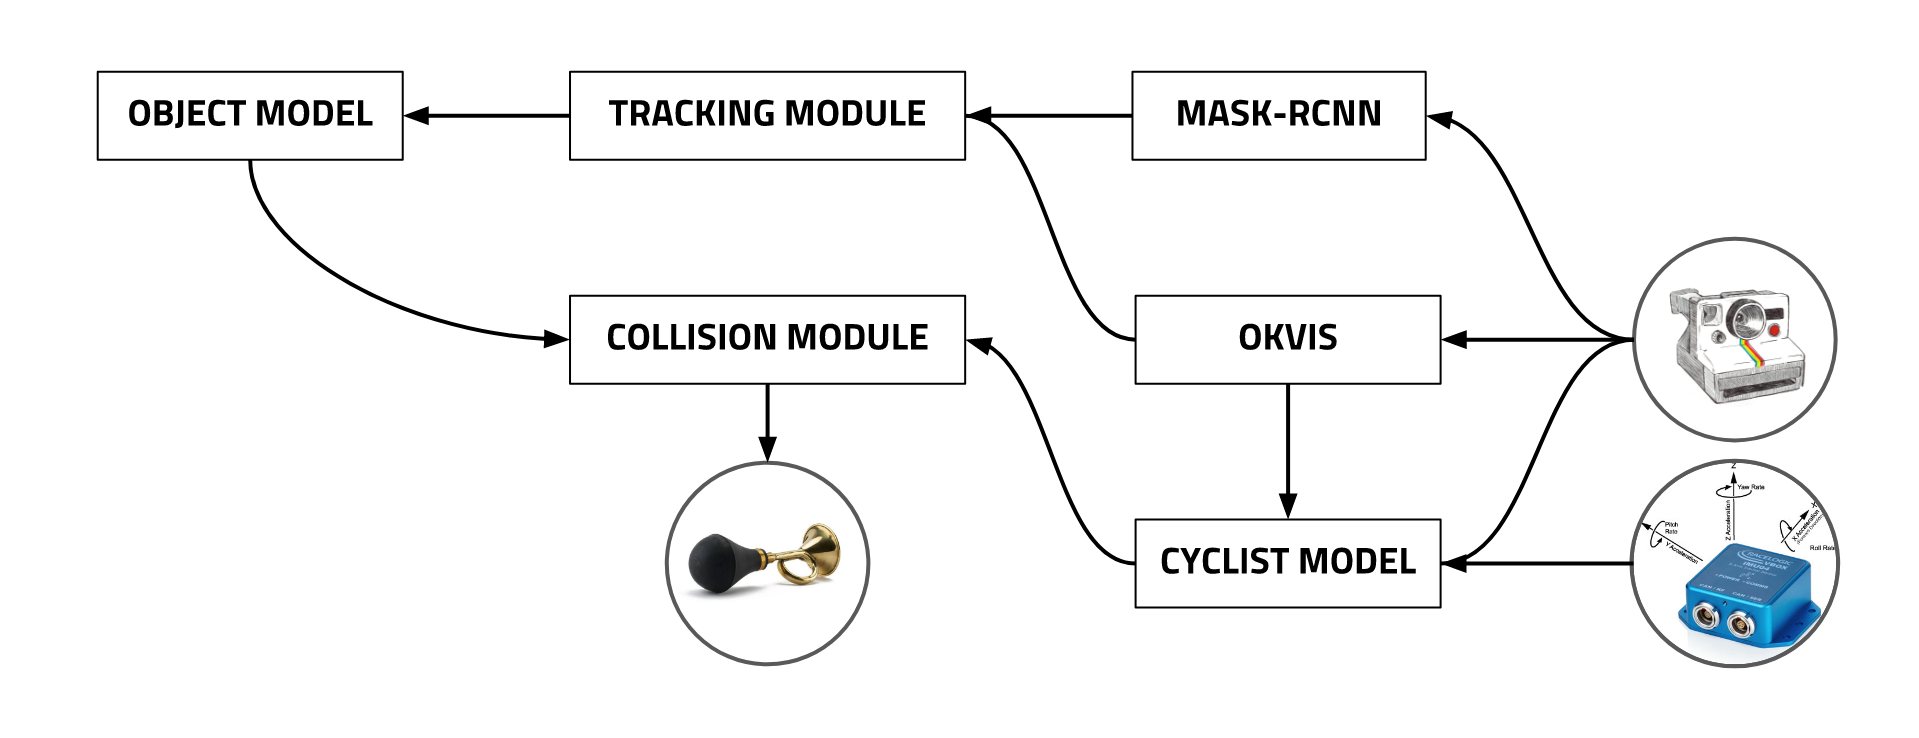
\includegraphics[width = 1.0\hsize]{figures/software_architecture.png}
	\caption{System Design}
	\label{software_soln1}
\end{figure}


\paragraph{System Evaluation}
This section describes the potential problems with the system, and includes an image sequence from a staged hazard. The final system can be seen to detect a crossing pedestrian and determine the collision is likely.

\paragraph{Conclusion}
This chapter discusses and summarises the system, it also suggests further areas of research if the system is to be taken further.

\paragraph{Ethics}
The final section discusses any ethical issues within the project and contains a completed ethical checklist.


\newpage



\chapter{Background}
\section{Background, Computer Vision}\label{comp_vis_back}
\subsection{Deep Learning Preliminaries} \label{dlp}
Computer vision and its applications has been revolutionised recently by Deep Learning frameworks. These have led to super-human accuracy in image recognition, for example Inception v3 \cite{Szegedy_2016_CVPR}, release in 2016, reached a 3.46\% error rate on the ImageNet \cite{ILSVRC15} dataset. This is known as an image classification task; the photo contains one object in the dataset and that object generally occupies the majority of the frame. Similar networks are used with additional features for image detection and segmentation which are integral to detecting moving objects such as pedestrians and vehicles in an urban environment.
\newline\newline
The current state-of-the-art methods in computer vision use a form of neural network. These networks are characterised by a series of non-linear nodes that are organised in layers. At each layer the network learns progressively abstract and higher-level features of the image to be detected until the final (usually dense layer) which determines the predicted class. Therefore the 'depth' of a neural network often refers to the number of layers and hence the inherent complexity of features that a network can learn. This is, however, only a basic representation of the problem and some clever and shallower architectures are able to outperform deeper networks. It is important to note that the depth and width, more specifically the number of parameters in the model generally reduces speed of prediction and increases the memory required to store/load the model into RAM. This is of little consequence in most applications, however for the limited computational power that can be carried on a bicycle it will be of concern in this report.

\subsection{Convolutional Networks} \label{Cnn_section}
A CNN generally contains convolutional, pooling, fully connected and normalisation layers. This form of network became particularly popular in computer vision after Geoffrey Hinton's 2012 paper \cite{GH_CNN}, with an ImageNet classification error of c.16\%, significantly lower than the state-of-the-art at the time which was 26\%. Convolutional networks use the assumption that each input is an image and therefore certain properties can be encoded into the architecture of the network. This allows a significant reduction in the number of tunable network parameters.
\newline \newline
A regular neural network, as mentioned earlier Section \ref{dlp}, contains a number of fully connected layers i.e. each neuron in a layer is connected to every neuron in the previous and next layers respectively. However convolutional neural networks are arranged in three dimensions: width, height, depth (Figure \ref{CNNvsNN}). In this architecture the neurons in a layer are only connected to some of the layer before, unlike in the fully connected case, this significantly reduces the number of parameters \cite{StanfordCS231_1}.

\noindent \begin{figure}[h!]
	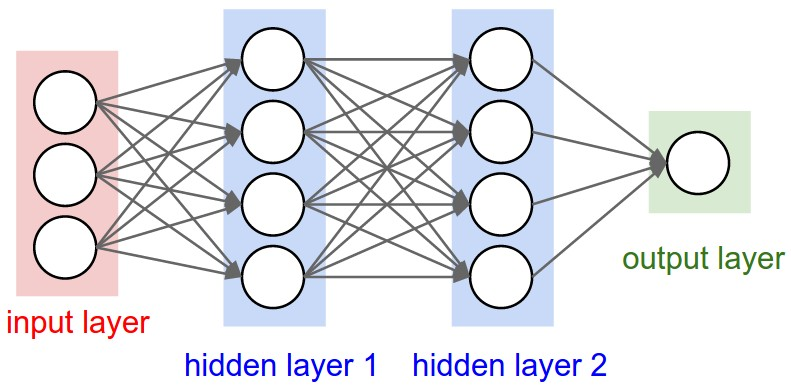
\includegraphics[width = 0.5\hsize]{./figures/neural_net2.jpeg}
	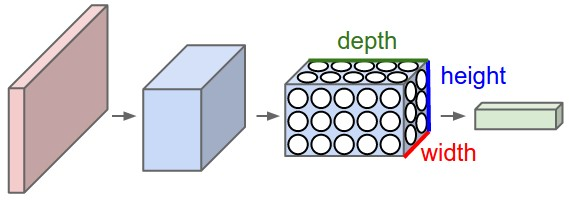
\includegraphics[width = 0.5\hsize]{./figures/cnn.jpeg}
	\caption{Regular Neural Network (Left) \cite{StanfordCS231_1} , CNN (right) \cite{StanfordCS231_1}.}
	\label{CNNvsNN}
\end{figure}

\subsubsection{Convolutional Layers}
A convolutional layer learns a set of filters, each filter is compact in size, say ($7 \times 7 \times 3$). This filter slides (convolves) over the image, then a dot product is taken between the filter values and the inputs to that filter (Figure \ref{CNN_filter}). The filter slides across with a respective stride, which is a hyperparameter, a stride of one equates to moving one pixel across at a time. A convolutional layer is therefore able to pick up features such as a corner, or higher level features such as the texture of fur. This process creates a 2D activation map containing the response of the filter at each position on the input volume. A number of filters are passed over and a number of activation maps are created, relating to the layer depth which is a tune-able hyperparameter.

\noindent \begin{figure}[h!]
	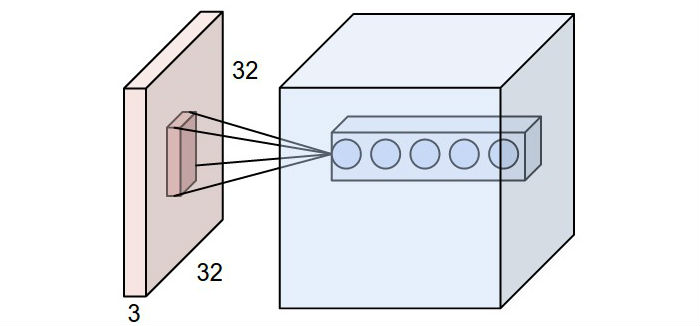
\includegraphics[width = 0.5\hsize]{./figures/conv_filter.jpg}
	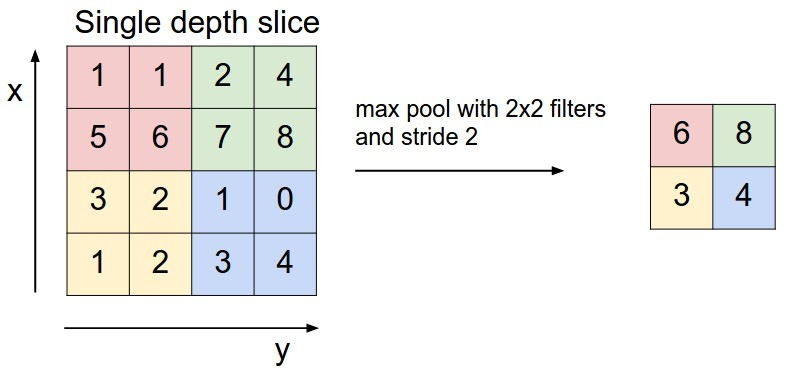
\includegraphics[width = 0.5\hsize]{./figures/maxpool.jpeg}
	\caption{CNN Filter (left) \cite{StanfordCS231_conv_filter}, Max Pooling \cite{StanfordCS231_max_pool}}
	\label{CNN_filter}
\end{figure}

\subsubsection{Pooling Layers}
Pooling layers are used to reduce the number of parameters in a network. This is a much debated topic, Geoffrey Hinton's paper \cite{DBLP:journals/corr/abs-1710-09829} dicusses the problems of convolutional networks in his 2017 paper and especially focuses on the disadvantages of pooling layers. It is however a current, although fading, method of parameter reduction. For the purposes of optimising network architecture for smaller hardware such as is portable on a bike this is still a recognised and useful method.
\newline \newline
A pooling layer such as that depicted in (Figure \ref{CNN_filter}) passes a kernel over the input (much like in a convolutional layer) and at each spacial location it calculates a metric. For example, max pooling takes the largest value contained within the kernel grid at each consecutive spacial location. This process reduces the input size with respect to the kernel size and the implemented stride.

\subsection{Image Detection} \label{Image_det}
Image detection is an area of research that uses the CNN networks described in Section \ref{Cnn_section}. This is, however, a more difficult task as there can be multiple objects/classes of interest within one image. A naive approach to this problem would be to slide a window across an image and classify at each location. When the network classifies, say a cat at a particular window location it is likely that a cat is located in that area.
\newline \newline
Although the aforementioned approach is valid it would be very slow, not only would it be needed to slide the window over the whole image, the size of the window would also need to be varied. The network cannot know the area of the photo that the object occupies and therefore what size to make the window. There are a number of differing approaches to this problem R-CNN \cite{DBLP:journals/corr/GirshickDDM13} and other later iterations vs YOLO (you only look once) \cite{DBLP:journals/corr/RedmonDGF15}. The R-CNN approach is very similar to the vanilla, naive solution, discussed above (commonly known as exhaustive search) and is used by later techniques for instance segmentation.


\subsubsection{R-CNN} \label{rcnn}
R-CNN, proposed by Ross Girshick et al. \cite{DBLP:journals/corr/GirshickDDM13} in 2014, incorporates a region proposal method. This process produces 2000 proposals which are then passed through a large CNN, and each region is classified using class-specific linear SVMs. This process equates to a 53.7\% mean average precision (mAP) compared to 35.1\% by state-of-the-art methods at the time. In addition to this performance gain the system doesn't rely on far more complicated ensemble methods.
\newline \newline
The region proposal method used is called selective search \cite{Uijlings2013}, this uses a fast segmentation algorithm by Felzenszwalb \cite{Felzenszwalb2004} followed by a greedy algorithm to iteratively group regions together using similarity metrics. The four metrics proposed in the paper are $s_{colour}$, $s_{texture}$, $s_{size}$, $s_{fill}$  the aim is to use a number of metrics to pick up the differences between regions during the growth period and also limit one region's growth at the expense of others (hence the size metric).

\noindent \begin{figure}[h!]
	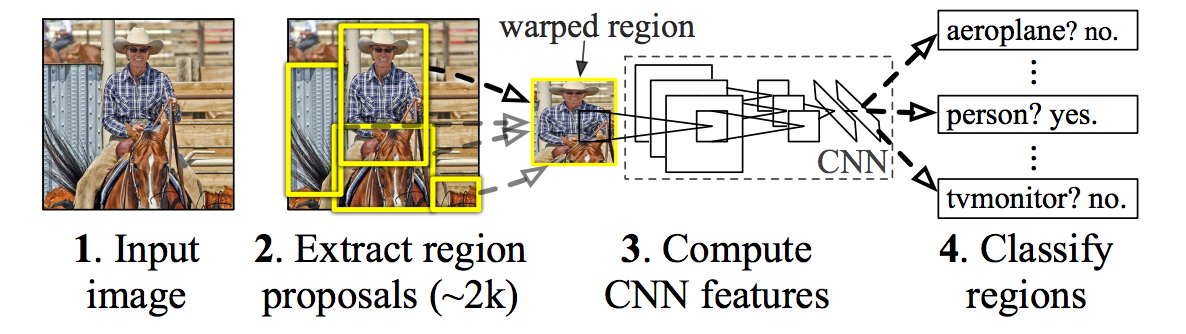
\includegraphics[width = 1.0\hsize]{./figures/region_prop.png}
	\caption{R-CNN Region Proposal \& Architecture \cite{DBLP:journals/corr/GirshickDDM13}}
	\label{Selective_search}
\end{figure}

The results of the region proposal (Figure \ref{Selective_search}) are a series of windows that are likely to contain an object. These are then simply warped to $227 \times 227$ pixels to fit the input dimension's of the CNN network that follows, containing five convolutional layers and two fully connected layers. The output of the CNN is then fed as a 4096 dimensional feature vector to a set of trained SVMs, one for each class, that are used to score the likelihood for that class. This approach is slow at 13s/image on a GPU and 53s/image on a CPU, the separation of a CNN and SVM is peculiar and adds to this timescale. A later iteration of this method Fast-RCNN is discussed in Section \ref{Fast_RCNN}.

\subsubsection{Fast-RCNN} \label{Fast_RCNN}

R-CNN performs a CNN forward pass for each region proposal and does not share computation between regions \cite{DBLP:journals/corr/Girshick15}. Spacial pyramid pooling networks (SPPnet) \cite{DBLP:journals/corr/HeZR014} are designed to mitigate this problem by creating a feature map (which is always the same shape) from an input image and then classifying each object proposal from a vector extracted from the shared feature map. This paper still uses a multiple-stage classification pipeline but is a marked improvement on R-CNN with regards to speed. 
\newline \newline
Fast-RCNN uses the SPPnet concept but also incorporates a single-stage pipeline. The process inputs an image and multiple RoIs into a fully convolutional network (Figure \ref{Fast_RNN_fig}). Each RoI is then pooled into a fixed-size feature map as in SPPnet and then mapped to a feature vector by fully connected layers. As can be seen in Figure \ref{Fast_RNN_fig} the network then branches into 2 separate outputs, one 4-point regression output of the bounding box location and a K-size classification output, where K is the number of object classes. The model therefore must contain a multi-task loss function that accounts for both bounding box and softmax loss (Equation \ref{multi-task_loss}).

\begin{equation}
\label{multi-task_loss}
L(p,u,t^{u},v) = L_{cls}(p,u) + \lambda[u \geq 1]L_{loc}(t^{u},v)
\end{equation}
in which $L_{cls}(p,u) = -log(p_{u})$ is the log-loss for true class $u$, and $L_{loc}$ is the bounding box regression loss defined as:

\begin{equation}
\label{bbox_loss}
L_{loc} = \sum_{i\in \{x,y,w,h\}}smooth_{L_{1}}(t^{u}_{i}-v_{i}),
\end{equation}
in which

%TODO
\begin{equation}
\label{multi-task_s}
smooth_{L_{1}} = 
\begin{cases}
0.5x^{2} \textnormal{if} x < 1 \\
|x| - 0.5  \textnormal{otherwise} \\
\end{cases}
\end{equation}
is a $L_{1}$ loss. This architecture allows for fast training with the forward pass of the network and therefore processes images 146$\times$ faster than R-CNN due to sharing computation between layers and the improved pipeline design. 

%TODO
\noindent \begin{figure}[h!]
	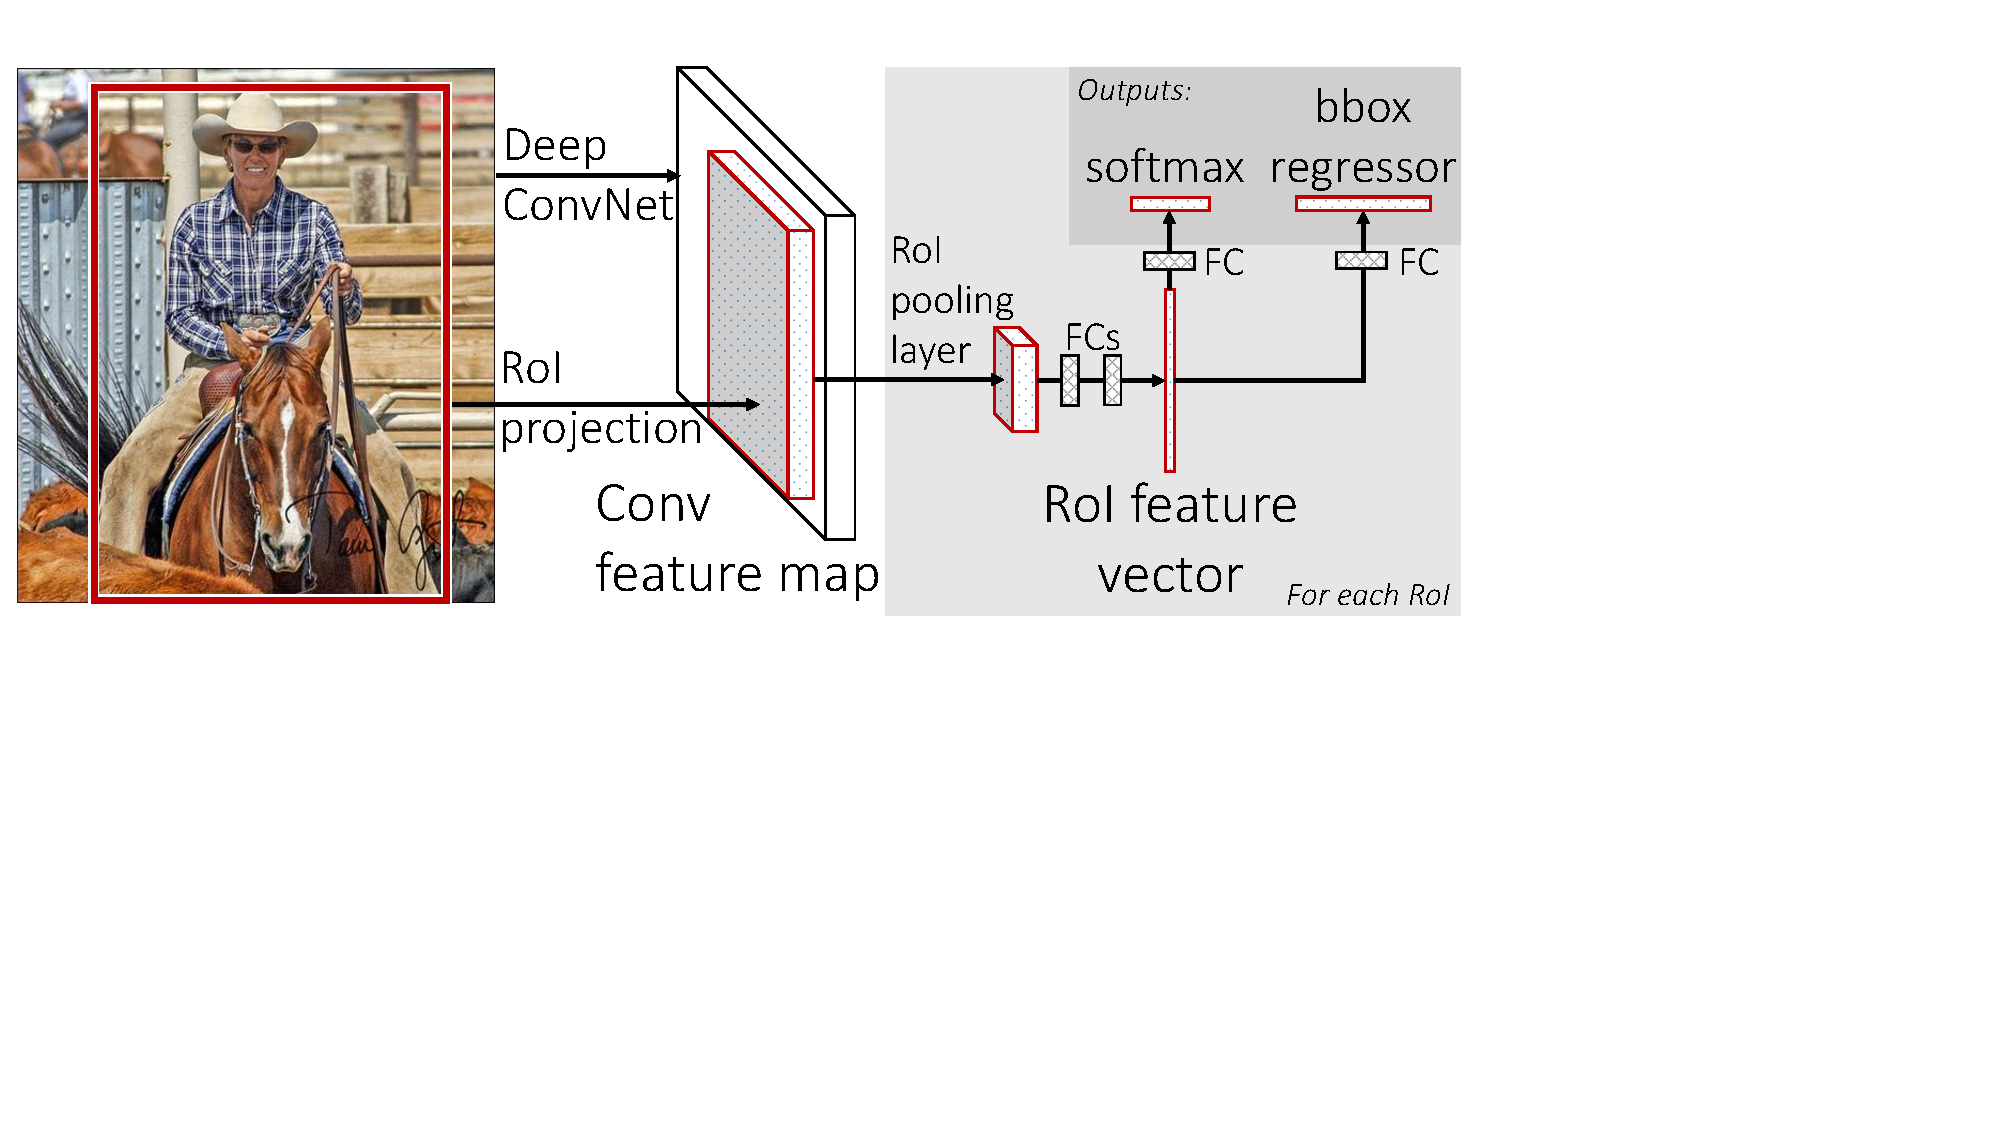
\includegraphics[trim={0 22em 22em 3em},clip,width = 1.0\hsize]{./figures/arch.pdf}
	\caption{Fast R-CNN Architecture \cite{DBLP:journals/corr/Girshick15}}
	\label{Fast_RNN_fig}
\end{figure}

Figure \ref{Fast_RNN_fig} depicts the network architecture, this incorporates an RoI pooling layer which maps the convolutional feature map from an RoI (created by selective search) to a fixed extent feature map of a set $H \times W$, where $H$ and $W$ are layer hyperparameters. Each RoI is a rectangular window defined by a tuple of four elements ($r,c,h,w$), where ($r,c$) specify the top left corner and ($h,w$) the width. RoI max pooling then divides the RoI window into a grid and then max-pools each grid into the corresponding output cell. The size of the grid is proportionate to the RoI and so the output shape is constant regardless of RoI input size. 

\subsubsection{Faster R-CNN} \label{Faster_rcnn}
Although the previous method \cite{DBLP:journals/corr/Girshick15} removed the need for a multi-stage classification pipeline (CNN and SVM), it still relies on the selective search \cite{Uijlings2013} method for region proposal. This part is now the computational bottleneck that slows down the process. Faster R-CNN proposed by Ren et al. \cite{DBLP:journals/corr/RenHG015} seeks to alleviate this issue by combining region proposal into the CNN. The paper suggests the use of a region proposal network (RPN) to produce the RoIs used later in the network. 

%TODO sort out grphic keep only (c)
\noindent \begin{figure}[h!]
	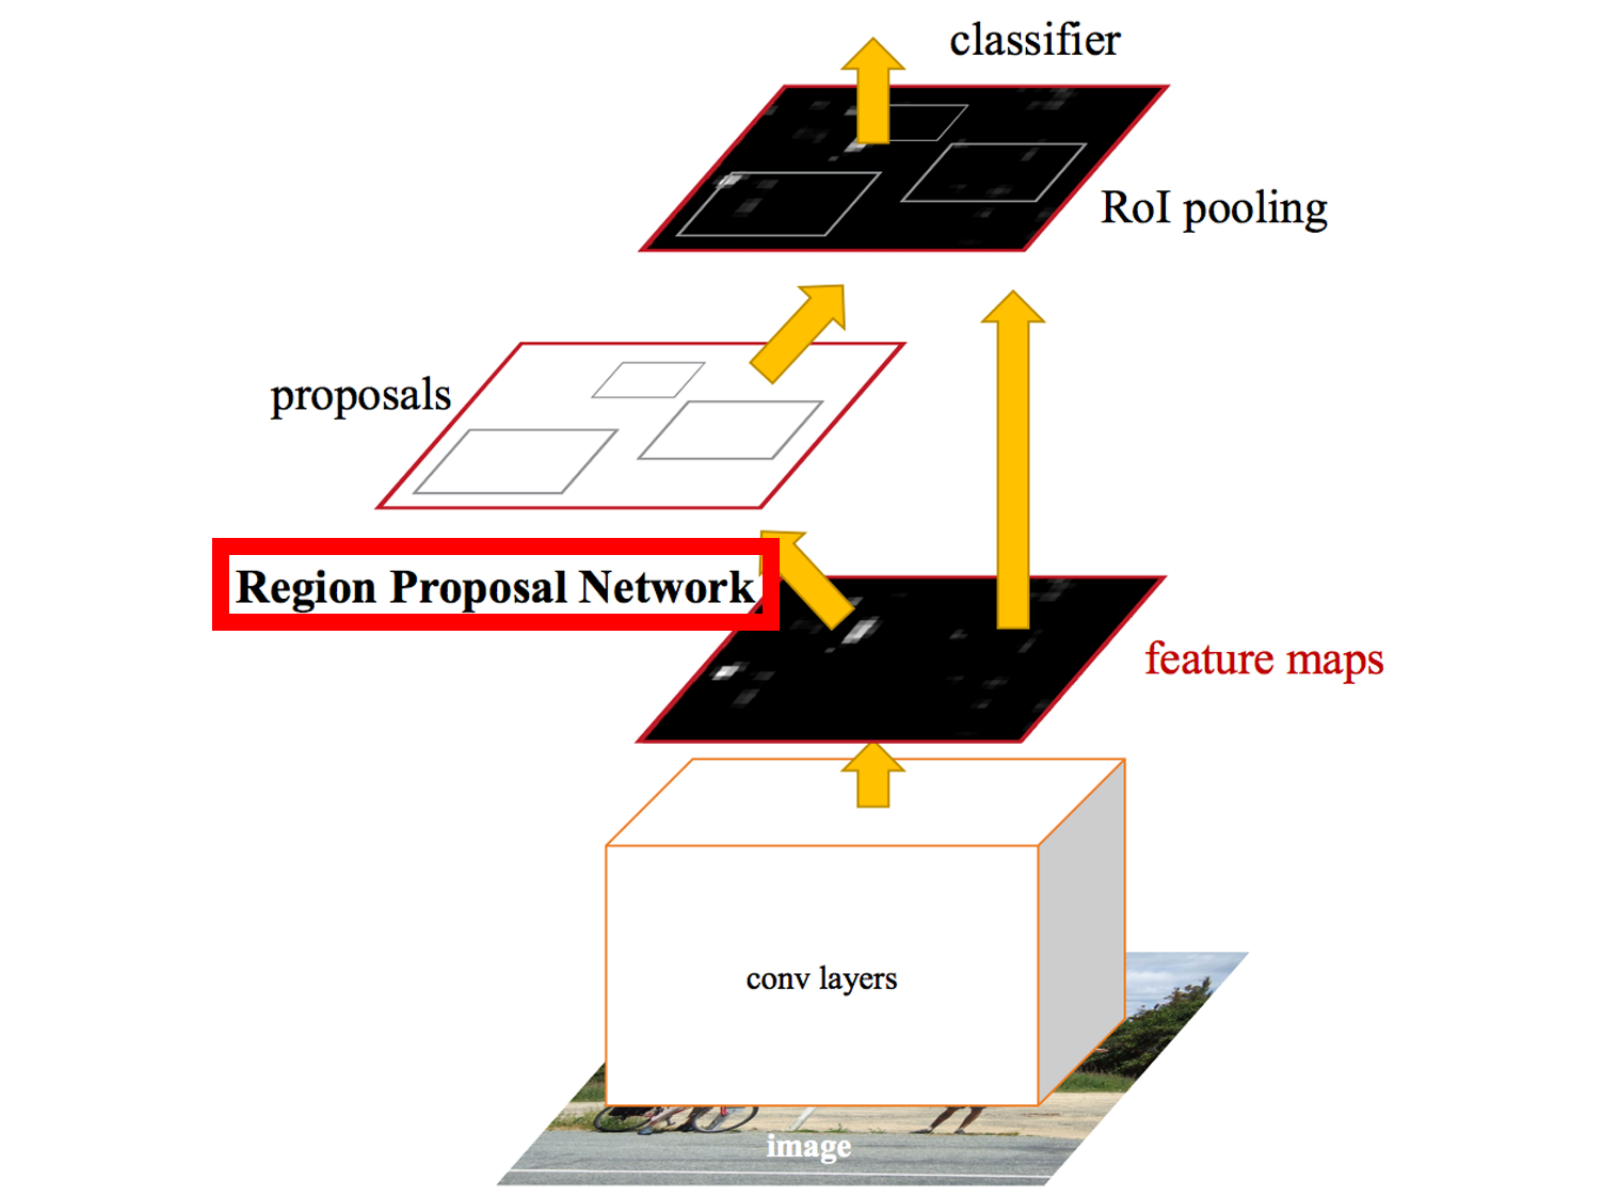
\includegraphics[width = 0.45\hsize]{./figures/faster.png}
	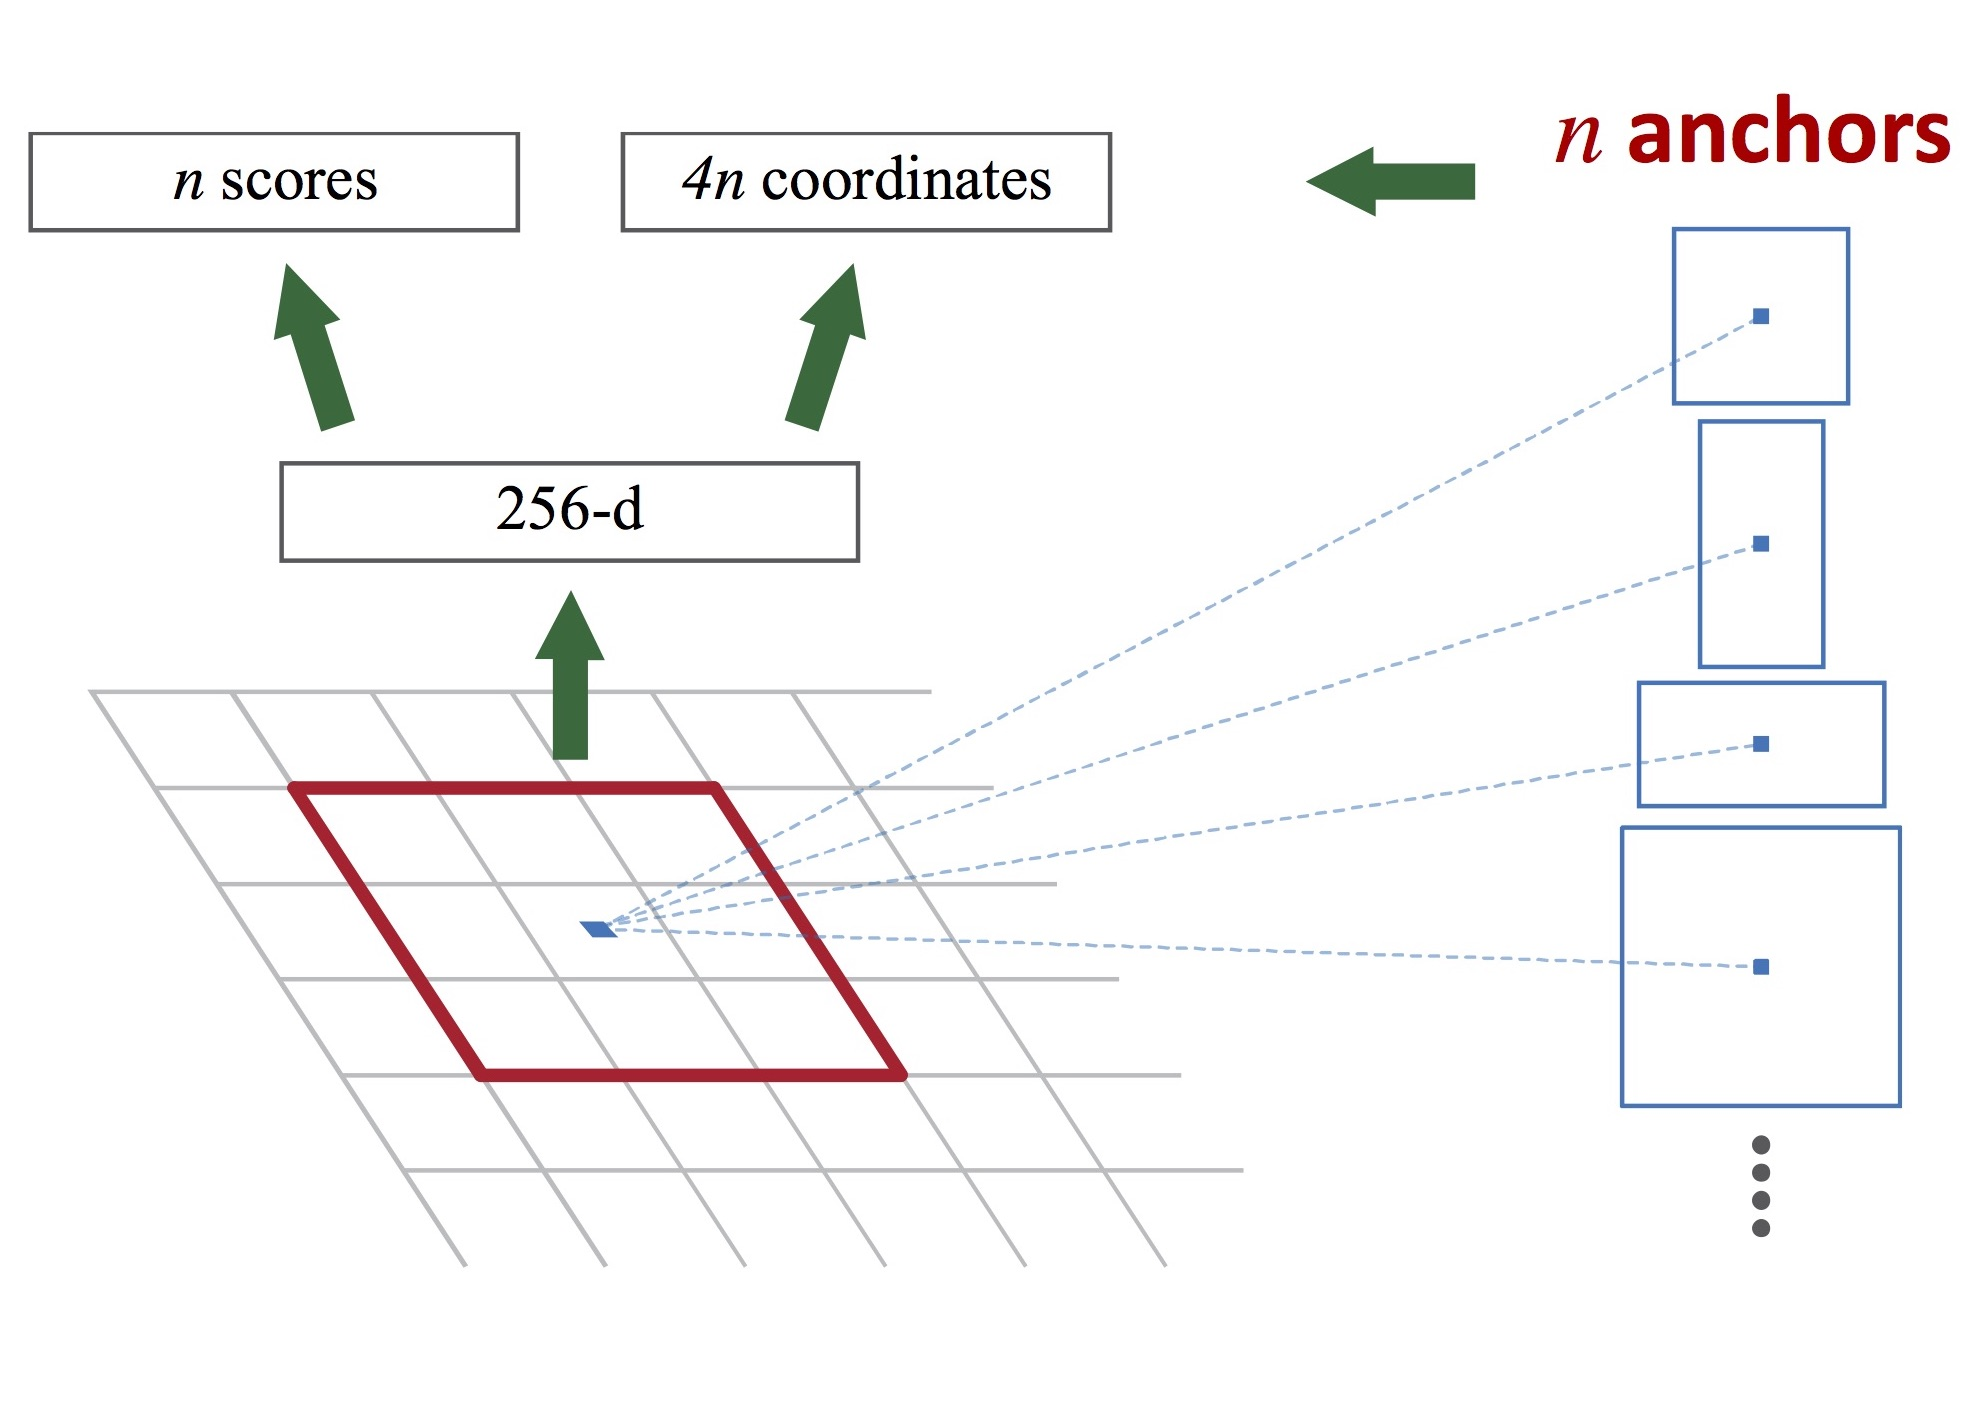
\includegraphics[width = 0.45\hsize]{./figures/rpn_faster.jpg}
	\caption{Fast R-CNN Architecture \cite{DBLP:journals/corr/Girshick15}}
	\label{Faster_rnn_fig}
\end{figure}

The region proposal network (RPN) outputs a set of rectangular object proposals, each of these proposals has an objectiveness score i.e. how likely the network thinks the proposal contains an object. This part of the network comes after a number of convolutional layers (in this paper 5 or 13 such layers). The region proposals are then created off the feature map from these layers by sliding a smaller network of size $n \times n$ over the convolutional feature map (Figure \ref{Faster_rnn_fig}). At each sliding window location a number of region proposals are predicted simultaneously. These consist of 3 aspect ratios and 3 scales, therefore 9 total region predictions or anchors at each location. The network is then followed by two sibling $1 \times 1$ convolutional layers, one for $reg$ (region proposal) and one for $cls$ (probability of object or not). The $reg$ layer outputs 4$k$ results, which represents the encoding coordinates of the $k$ boxes and the $cls$ later scores the probability that there is an object or no object in each proposal, therefore cls has $2k$ outputs. This results in a convolutional layer output of depth 9.
\newline \newline
The loss for the network is calculated from two metrics, the output of the $reg$ layer is a binary, i.e. positive example, or not. A positive example is defined by how much the box overlaps with the ground truth box of the object and so an IoU (Intersection-over-union) overlap $> 0.7$ is considered a positive example and an IoU $< 0.3$ is considered a negative label. For the first positive case, if no positive examples are found, the boxes with highest IoU  are labelled positive. With this it follows that:

\begin{equation}
\label{multi-task_loss_fast_rcnn}
L(\{p_{i}\},\{t_{i}\}) = \frac{1}{N_{cls}} \sum_{i} L_{cls}(p{i},p_{i}^{*}) + \lambda \frac{1}{N_{reg}} \sum_{i}p_{i}^{*} L_{reg}(t_{i},t_{i}^{*})
\end{equation}

Where $i$ is the anchor index, $p_{i}$ is the predicted probability of anchor $i$ containing an object. The ground truth label $p_{i}$ is denoted as a 1 for a positive anchor and 0 for a negative therefore $L_{reg}$ is only activated for a positive example, $t_{i}$ and $t_{i}^{*}$ represent the 4 coordinates of the bounding boxes, and $L_{cls}$ is the classification loss. The two terms are normalised ($N_{cls}$ and $N_{reg}$) and balanced by a weighting parameter $\lambda$. The final term to discuss, the bounding box regression is calculated, simply, as follows:


\begin{align*}
\label{bounding_box_loss}
t_{x} = (x-x_{a})/w_{a}, \quad t_{y} = (y-y_{a})/h_{a},\\
t_{w} = log(w/w_{a}), \quad t_{h} = log(h/h_{a}), \\
t_{x}^{*} = (x^{*}-x_{a})/w_{a},\quad t_{y}^{*} = (y^{*} - y_{a})/h_{a}, \\
t_{w}^{*} = log(w^{*}/w_{a}), \quad t_{h}^{*} = log(h^{*}/h_{a})
\end{align*}

where $x$, $y$, $w$, and $h$ are the box centre coordinates plus width and height. Predicted box, and anchored box are denoted by $x$, $x_{a}$, $x^{*}$ (likewise for $y$, $w$, $h$).
\newline \newline
Finally after the regions have been proposed, c.6000 per image, some regions overlap with others, and so, to reduce redundancy non-maximum supression is used on their $cls$ score with an IoU threshold of 0.7 to leave around 2000 proposals per image. Non-maximum supression is a technique that sets all neighbouring areas to zero around a local maximum and hence only keeps the maximum value and suppresses the others.

\subsection{Image Segmentation}\label{image_seg}
Unlike the image detection problem described in Section \ref{Image_det}, this task aims to segment an image on a pixel-by-pixel basis into respective classes (Figure \ref{cityscapes_data}). A conventional classification network takes an image and outputs a prediction of which class the image is i.e. a vector of probabilities or a `score'. This process uses fully-connected layers to produce the final output vector which throws away important spacial information used in a segmentation task. Therefore Long et al. \cite{DBLP:journals/corr/LongSD14} propose converting these final layers to convolutional layers, maintaining the spacial information and creating a heatmap output (Figure \ref{cityscapes_data}).

\noindent \begin{figure}[h!]
	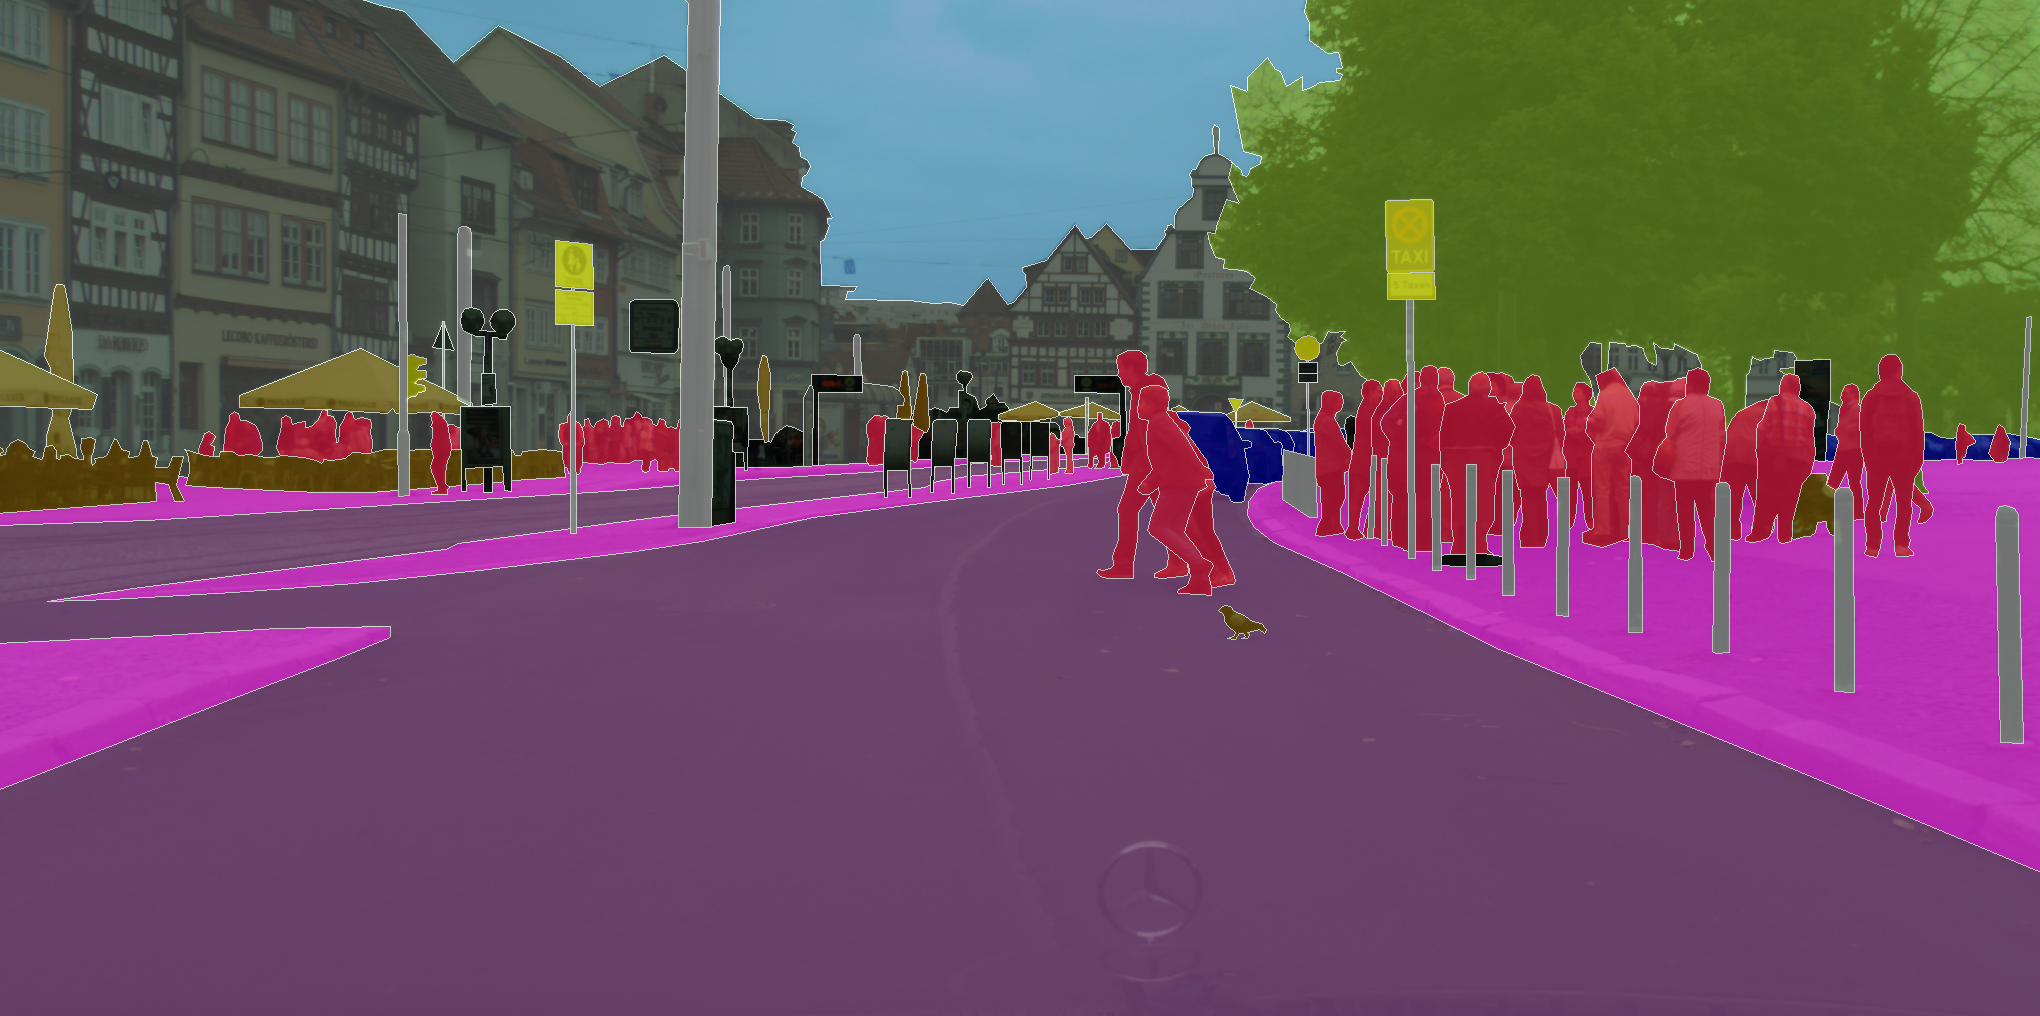
\includegraphics[width = 0.5\hsize]{./figures/image_seg1.png}
	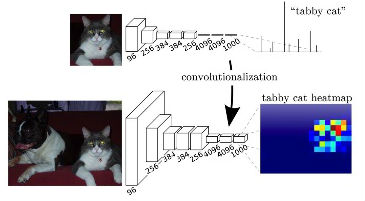
\includegraphics[width = 0.5\hsize]{./figures/sem_im_seg1.jpg}
	\caption{Image Segmentation \cite{DBLP:journals/corr/CordtsORREBFRS16}, Convolutional Heat Map \cite{DBLP:journals/corr/LongSD14}}
	\label{cityscapes_data}
\end{figure}

The heatmaps produced from the network then need to be upsampled from their respective dimensions to that of the output image. This process is essentially a reverse or deconvolution. Upsampling, therefore, with factor f is convolution with a fractional input stride of 1/f. Essentially each filter is placed on the output image and then multiplied by the input pixel. Hence the image increases in size depending on stride and kernel size as one pixel value is interpolated over a grid. The final problem therefore is how to choose the filter values, this can be done in a number of ways but the main accepted approach is to simply learn them as part of the tuning process.
\newline \newline
An important concept is that of patchwise training which feeds the network a number of patches from an input image (small patches surrounding objects of interest) instead of an entire input image. This both helps to balance the classes, ensures the input has enough variance, and is a correct representation of the input set. However, this paper argues that this can be done from a fully convolutional training regime with incorporating a DropConnect-like mask \cite{Wan:2013:RNN:3042817.3043055} between the output and the loss. A DropConnect mask is similar to the proposed regularisation technique of Dropout \cite{JMLR:v15:srivastava14a} except that it randomly sets the network weights to 0 rather than the activation functions. This, on the output layer (connected to the network loss) is found to have the same effect as patch-wise sampling in Long et al.'s paper.
\newline \newline
Although conventional proven classification architectures performed to state-of-the-art when modified for segmentation (56.0 mean IU), Long at al. \cite{DBLP:journals/corr/LongSD14} go on to design a bespoke network that achieves 62.7 mean IU. Mean pixel intersection over union (Mean IU) is a standard performance metric where the mean is taken over all classes, including the background. The paper describes a network architecture that uses skips \cite{Bishop:2006:PRM:1162264}. Skips allow predictions from lower-level coarser layers to interact with finer, latter layer predictions. This lets the model make local predictions (finer) within the context of the global structure (coarser). This addition made for a marked increase in performance by simply up-sampling earlier layers and summing with latter layer outputs for a final image prediction.

\subsection{Instance Segmentation}
Instance segmentation is a problem that combines research in Sections \ref{Image_det} \& \ref{image_seg}, it aims to not only perform pixel-wise segmentation of classes but also determine instances of objects within and image. As discussed in Section \ref{mask_rcnn} there is a simple method of combining these networks into one simple classification pipeline.
\subsubsection{Mask R-CNN} \label{mask_rcnn}
Mask R-CNN was proposed by Facebook AI Research (FAIR) namely Kaiming He et al. in March 2017. It uses the Faster R-CNN network described in Section \ref{Faster_rcnn} which builds from advances in Sections \ref{rcnn}  \& \ref{Fast_RCNN}. The method works by simply adding a branch from the existing network for predicting segmentation masks as in Section \ref{image_seg} (Figure \ref{Mask_rcnn_arch}). The branch is a small FCN that is applied to each RoI for segmentation. There are a number of slight modifications to each approach to produce the final Mask R-CNN that are documented below.
\newline \newline

\noindent \begin{figure}[h!]
	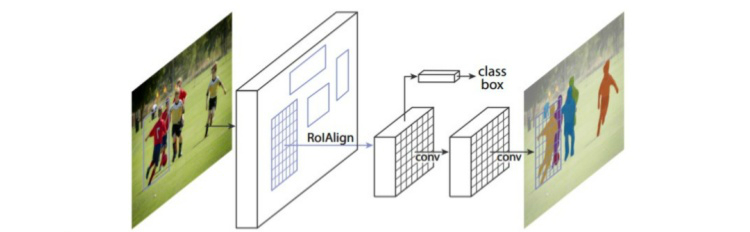
\includegraphics[width = 1.0\hsize]{./figures/mask_arch.jpg}
	\caption{Mask R-CNN \cite{DBLP:journals/corr/HeGDG17}}
	\label{Mask_rcnn_arch}
\end{figure}
%TODO nice binary mask per class photo
RoIs are produced from the RPN as in Faster R-CNN \cite{DBLP:journals/corr/RenHG015} then a $m \times m$ mask is predicted from each RoI without the use of a fully-connected (fc) layer and therefore keeps spacial information as in Section \ref{image_seg}. It was found during experimentation that it is preferable to decouple the class classification and the mask production of the network. This stops multiple classes disrupting each other during mask production, hence a mask is produced for each class. The class of each respective mask is then determined from the class output branch and that binary mask is selected. 
\newline \newline
The loss function for the network must now incorporate the three different branches; mask, class prediction, and bounding-box prediction (Equation \ref{maskrcnnloss}). 

\begin{equation}
\label{maskrcnnloss}
L = L_{cls} + L_{box} + L_{mask}
\end{equation}

where $L_{cls}$ \& $L_{box}$ are identical to Section \ref{Fast_RCNN}. The mask branch loss is determined by a per-pixel sigmoid between the ground-truth class ($k$) and the corresponding $k$th binary mask (excluding other classes) and is calculated with an average binary cross-entropy loss.
\newline \newline
RoI pool as discussed in Section \ref{Fast_RCNN} is modified in this approach. Instead of subdividing an RoI into discrete regions e.g. a grid of $4 \times 5$ cells. An RoI does not always divide equally into these grid cells and so rounding of grid sizes is needed, this quantisation of sub-windows can cause misalignments of the RoI and extracted features. The new RoIAlign layer introduced in this paper mitigates this problem by not rounding grid-cells. Mask R-CNN uses bi-linear interpolation (linear interpolation with 2d) to compute the exact values of input features.
\newline \newline
This network architecture is the final piece required to segment the images provided by the camera and is the model used in the cycling system. The next section will go on to talk about the other networks used for things such as position prediction.
\subsection{Recurrent Neural Networks (RNN):}

\paragraph{Traditional RNN Layer:}A normal dense network layer has no memory of the previous features that pass through it. This would mean that in order to classify a sequence the data must be passed through the layer simultaneously. The advantage of a recurrent layer its ability to remember. A Long-Short Term memory (LSTM) layer has a weighted channel that inputs the output of the previous state as part of the next, see Figure \ref{rnn_unrolled} for more details. Each state $ \{ 1,2,...,t-1,t \}$ is connected to one another almost like a chain, the output of the cell at time $t$, from inputs $x_{t}$ is $h_{t}$.

\noindent \begin{figure}[h!]
	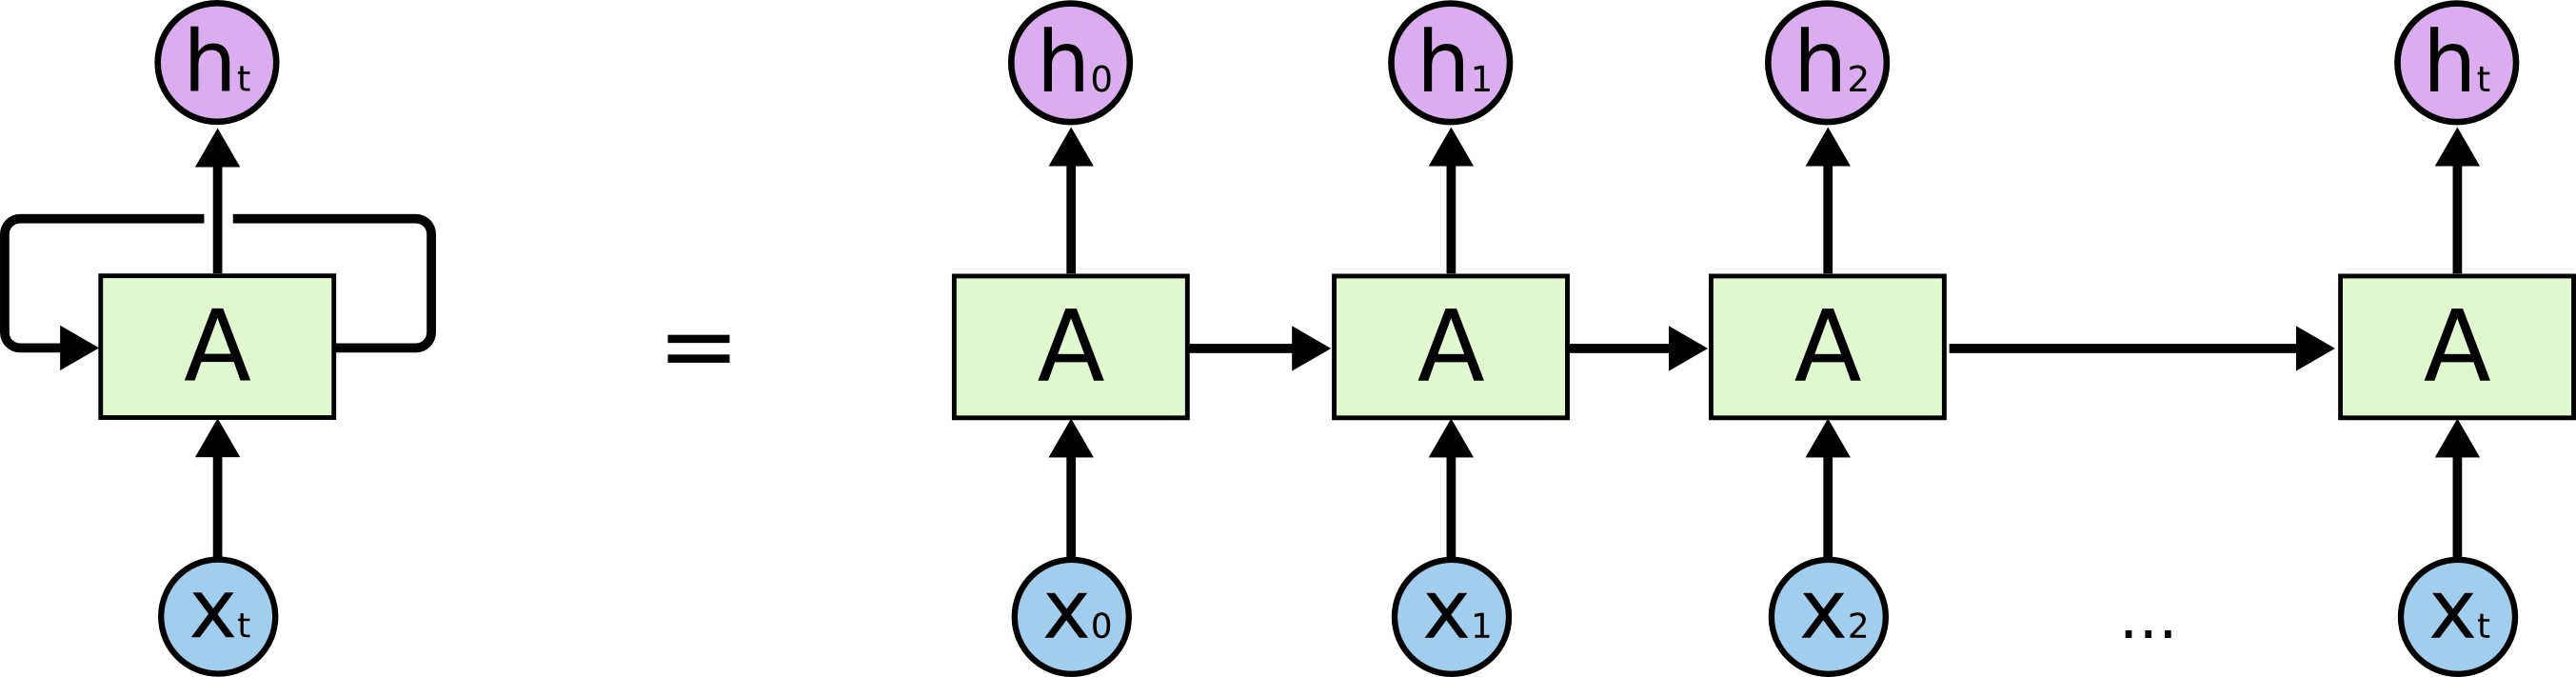
\includegraphics[width = 1.0\hsize]{./figures/RNN-unrolled.png}
	\caption{A Recurrent Layer \cite{Christopher_Olah_Blog}}
	\label{rnn_unrolled}
\end{figure}

The main issue with this recurrent layer is how far back the network is capable of remembering. In short sequences the information will pass effectively through the chain, but often in longer sequences the network is less capable of remembering previous states. 

\subsubsection{Long-Short Term Memory (LSTM) Layer} 
LSTM layers are far better at remembering, and do not get the vanishing gradient problem that RNN layers are subject to. LSTMs contain a cell state which passes through the layer, a forget, input, and output gates. These gates determine whether to modify the cell state of the layer, this acts as the memory of the later and is similar to the links in the RNN chain (Figure \ref{rnn_unrolled}). The gates contain sigmoid functions which can evaluate between to 0 and 1, and determine how much of a component is to be let through.

\noindent \begin{figure}[h!]
	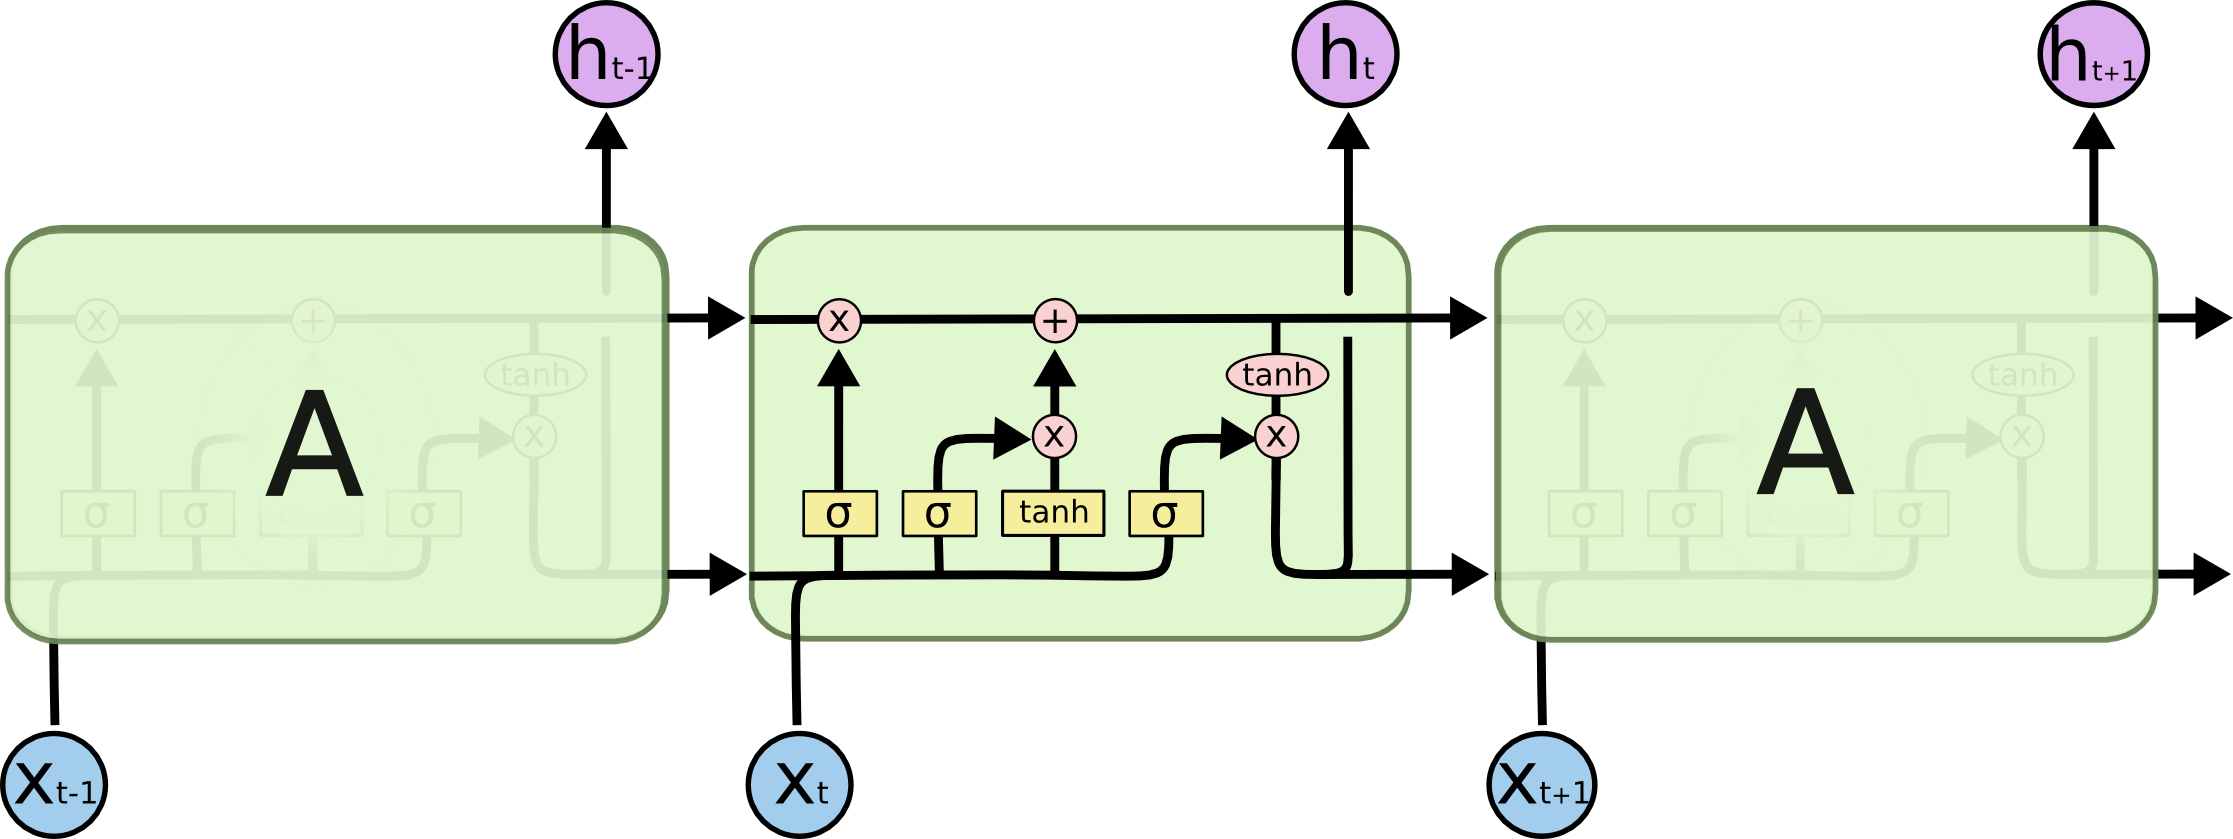
\includegraphics[width = 1.0\hsize]{./figures/LSTM3-chain.png}
	\caption{A LSTM (Long-Short Term Memory) Layer \cite{Christopher_Olah_Blog}}
	\label{lstm_fig}
\end{figure}


\paragraph{Forget Gate:}
The forget gate determines how much of the cell state to keep by looking at $h_{t-1}$ and $x_{t}$. The gate simply acts like a network layer, multiplying inputs by a weight, adding a bias and then passing the result through the activation (Sigmoid) function (Equation \ref{forget_gate}). 

\begin{equation}
\label{forget_gate}
f_{t} = \sigma (W_{f} \cdot [h_{t-1},x_{t}] + b_{f})
\end{equation}

Once again $h_{t-1}$ is the output of the layer from the last state, $x_{t}$ is the layer input at time $t$.

\paragraph{Input Gate:} When the gate has determined what to forget from the last state it needs to decide what to add from the new state $x_{t}$ for a correct prediction $h_{t}$. This introduces the next gate in the system which combines an input sigmoid gate that decides which values of $x_{t}$ to add (Equation \ref{input_gate0}), and a $tanh$ section that creates the new vector $\tilde{C}_{t}$ to add to the current state $C_{t}$, Equation \ref{input_gate1}.



\begin{equation}
\mathit{i}_{t} = \sigma (W_{i} \cdot [h_{t-1},x_{t}] + b_{i})
\label{input_gate0}
\end{equation}

\begin{equation}
\tilde{C}_{t} = tanh(W_{C} \cdot [h_{t-1},x_{t}] + b_{C})
\label{input_gate1}
\end{equation}



The input gate and forget gate then influence the state via weighting $C_{t-1}$ by the forget metric $f_{t}$ and $\tilde{C}_{t}$ by the input scale, Equation \ref{input_gate2}.

\begin{equation}
C_{t} = f_{t} \times C_{t-1} + i_{t} \times \tilde{C}_{t}
\label{input_gate2}
\end{equation}

\paragraph{Output gate:} The final step of a LSTM is to decide the output. This involves deciding which parts of the cell state to output and scaling to (-1,1) via the use of another $tanh$ function, Equation \ref{input_gate3}.


\begin{equation}
o_{t} = \sigma (W_{o}[h_{t-1},x_{t}] + b_{o}) \\
h_{t} = o_{t} \times tanh(C_{t})
\label{input_gate3}
\end{equation}

\paragraph{Summary:}

The LSTM layer is highly effective at predicting sequences, it is used later within the system to predict where the bike will be in the future. It provides an effective and sufficiently complex method of modelling bicycle movement including determining from picture inputs the most likely path along a road that the bike will take. Now that the networks have been defined, they must be optimised to perform well at their respective tasks. Mask-RCNN is kept as default in this report but the prediction models architecture is bespoke and thus must be optimised for its use-case.
 
\subsection{Bayesian Optimisation of Layer Dimensions:}
In order to get the best network architecture, and hyper-parameters such as learning rate, it is possible to naively try combinations and record which performs the best. However, when trying to optimise networks efficiently it is better to provide a range of possible working parameters and optimise them in an informed and, more importantly, automated manner. Bayesian optimisation allows such a method and can quickly check the parameter space for a good combination to minimise the network loss. Bayesian optimisation uses an acquisition function which evaluates a Gaussian process. It is cheaper to evaluate a proxy function that approximates the true function rather than run the neural network. Hence it is a very fast and effective method of optimisation.

\paragraph{Gaussian Processes:}
In a typical regression sample, the aim is to determine the parameters to a function (or family of functions) that best describe some data. A Gaussian process involves making the assumption that a function can be described simply by an infinite number of points along a function $f(x) = [f_{1},f_{2},...f_{\infty}]$, a finite number of which are gaussian distributed. The aim is to then best approximate the relationship between these points via a covariance kernel $k(\cdot,\cdot)$ and a mean function $m(\cdot)$. A gaussian distribution is described by Equation \ref{gaus_dist} and a kernel function (Matern) by Equation \ref{matern}.

\begin{equation}
\begin{aligned}
p(x|\mu,\Sigma) = (2 \pi)^{\frac{D}{2}} | \Sigma|^{- \frac{1}{2}} e^{(- \frac{1}{2}(x- \mu)^{T} \Sigma^{-1}(x- \mu))}
\end{aligned}
\label{gaus_dist}
\end{equation}


\begin{equation}
\begin{aligned}
k_{Mat,3/2}(x_{i},x_{j}) = 
\sigma_{f}^{2} \bigg ( 1 + 
\frac{\sqrt{3}||x_{i}-x_{j}||}{\mathit{l}} \bigg )e^{ \big (-\frac{\sqrt{3}||x_{i}-x_{j}||}{\mathit{l}} \big )}
\end{aligned}
\label{matern}
\end{equation}

where $\mathit{l}$ is a hyperparameter that describes the smoothness of the data and $\mathit{\sigma_{f}}$ the amplitude of the latent function. An example of a Matern kernel is given in Figure \ref{matern_kernel_fig}.


\noindent \begin{figure}[h!]
	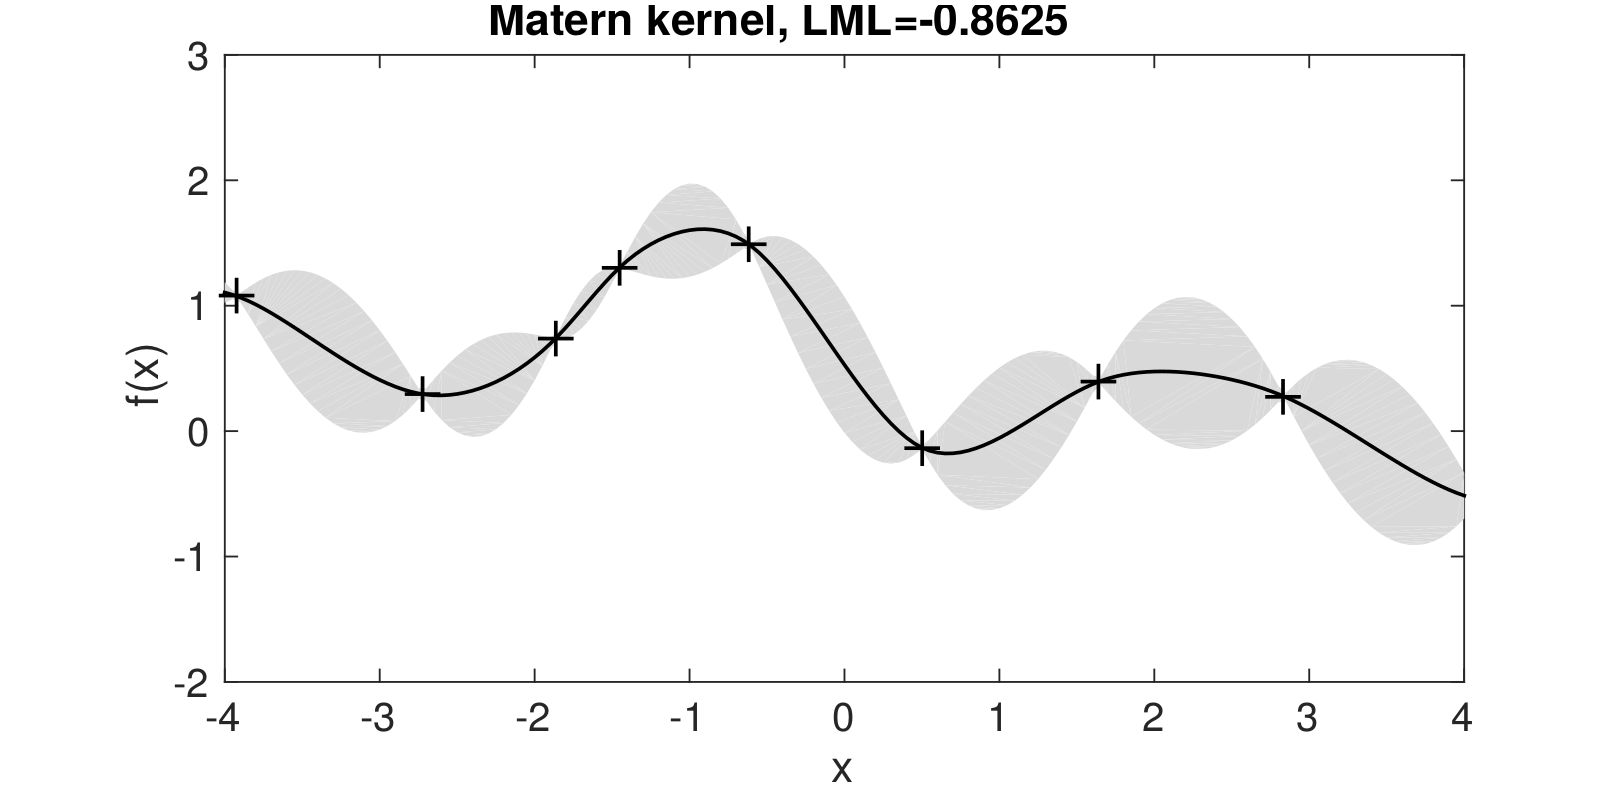
\includegraphics[width = 1.0\hsize]{./figures/Matern_Kernel.png}
	\caption{Gaussian Process: Matern Kernel \cite{Marc_Deisenroth_Notes}}
	\label{matern_kernel_fig}
\end{figure}

\paragraph{Bayesian Optimisation:}
Bayesian Optimisation is a process that can maximise a set of hyper-parameters with a reduced evaluation of the true function. It uses an acquisition function that balances state exploration and exploitation i.e. how much to search local minima for the best solution vs exploring for global minima. The true function (NN model) is evaluated and data collected to initialise the process. Then the acquisition function determines where to evaluate next in the true function by querying the proxy function. An example acquisition function, the lower confidence bound \cite{SrinivasNiranjan2010GPOi} is presented in Equation \ref{gp_lower_confidence}.

\begin{equation}
\begin{aligned}
\alpha(\mathbf{x}) = -(\mu(\mathbf{x}) - \mathit(k) \sigma (\mathbf{x})) \text{ , } k>0
\end{aligned}
\label{gp_lower_confidence}
\end{equation}


The lower confidence bound balances exploration of global minima by the covariance function and weighting $k$, which increases at each iteration, with exploitation of local minima with the mean function. The Bayesian optimisation process roughly translates to:\newline\newline
\begin{algorithm}[H]
	\DontPrintSemicolon
	\SetAlgoLined
	\setstretch{1.3}
	\SetKwInOut{Input}{Input}
	\SetKwInOut{Output}{Output}
	\underline{update\textunderscore matched\textunderscore rois} ($old$\textunderscore$matched,new$\textunderscore$matched,old$\textunderscore$frame,new$\textunderscore$frame)$\;
	\Input{ \texttt{\\}
		$parameters$ \tcp*[r]{A list of parameters to optimise}
		$parameter_limits$ \tcp*[r]{A list of ranges to optimise the parameters within}
		$function$ \tcp*[r]{A pointer to the function to optimise}
	}
	\Output{ \texttt{\\}
		$parameters$ \tcp*[r]{The optimal parameters}
	}
	\texttt{\\}
	\tcp{Note that if there are no objects in old frame $new$\textunderscore$frame.id$ = zeros}
	$D = [\{ x_{0},y_{0} \}]$ \tcc*[r]{Initialise the dataset}
	
	\ForEach(\tcc*[f]{For every not-matched new RoI}){$step \in iterations$}{
		$update \textunderscore gp(D[step-1])$ \tcc*[r]{Update the Gaussian process with data from the last step}
		$x_{step} = argmax(\alpha(x))$ \tcc*[r]{Evaluate the acquisition function for where to evaluate next}
		$y_{step} = function(x_{step})$ \tcc*[r]{Evaluate true function (NN model)}
		$D.append( \{ x_{step},y_{step} \} )$ \tcc*[r]{Add data to dataset}
	}
	$return (X_{best})$ \tcc*[r]{Return optimal parameters}
	\texttt{\\}
	\caption{Algorithm for Bayesian Optimisation}
	\label{alg:weights}
\end{algorithm}

\newpage

\section{Background, SLAM} \label{back_slam}
In order to detect collisions between the bike and obstacles the software must have an understanding of the global environment. The detection described in Section \ref{comp_vis_back} allows mapping, and tracking of dynamic objects in the frame, but distance, path prediction and eventually collision prediction rely strongly on an accurate understanding of 2.5-3D space.

\subsection{Sensors}
The sensors used in this project are an RGBD camera and an IMU. These are both available in the Intel Realsense Camera (ZR300, Figure \ref{realsense_camera}). This camera has a USB cable that both provides the power and sends camera information. An extension cable allows for a laptop to be attached to the camera, from a backpack whilst cycling. Potential problems with this setup are due to juddering of the bike on the road; this could cause tricky footage to analyse and data loss when the hard-drive is writing to disk. The latter issue can easily be solved by writing to an SSD while cycling.

\noindent \begin{figure}[h!]
	
\includegraphics[width = 1.0\hsize]{./figures/intel_realsense.jpg}
	\caption{Intel Realsense Camera (ZR300)}
	\label{realsense_camera}
\end{figure}

\subsubsection{Camera Distortion}
In order to fully understand the bike's location, the environment can be considered from two frames of reference, the world and camera frame. The camera, however, cannot be assumed to produce a perfect image and is hence prone to distortion - some types of camera distortion are shown in (Figure \ref{distortion}).


\noindent \begin{figure}[h!]
	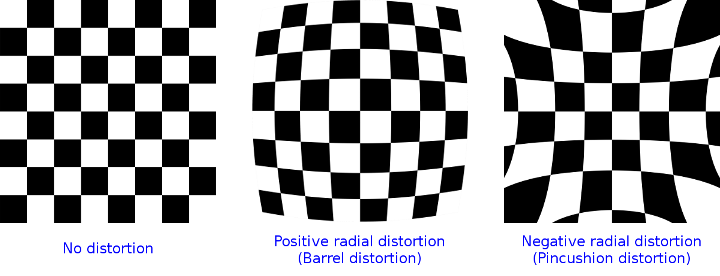
\includegraphics[width = 1\hsize]{figures/distortion_example.png} 
	\caption{No Distortion (left)\cite{opencv_camera_article}, Positive/negative radial distortion (middle/right)}
	\label{distortion}
\end{figure}

A well-known distortion model is "radial-tangential" distortion. As the name implies there is both a radial and tangential component to the distortion (Equation \ref{raddis}) 

\begin{equation}
r^{2} = x_{1}^{'2} + x_{2}^{'2} \\
\end{equation}
\begin{equation}
\mathbf{x''} = \mathbf{d(x')} = \frac{1 + k_{1}r^{2} + k_{2}r^{4}+k_{3}r^{6}}{1+ k_{4}r^{2} + k_{5}r^{4}+k_{6}r^{6}}
\begin{bmatrix}
x'_{1} \\[0.3em]
x'_{2}
\end{bmatrix}
+ 
\begin{bmatrix}
2p_{1}x'_{1}x'_{2} + p_{2}(r^{2} + 2x_{1}^{'2}) \\[0.3em]
p_{1}(r^{2} + 2x_{2}^{'2}) + 2p_{2}x'_{1}x'_{2}
\end{bmatrix}
\label{raddis}
\end{equation}



where $x'_{1},x'_{2}$ is the 3d point mapped to the unit plane in z, $k_{1}-k_{6}$ are radial distortion parameters, $p_{1},p_{2}$ are tangential distortion parameters. The model parameters can be determined during camera calibration.


\subsection{Camera to World Frame} \label{cam2world}

\subsubsection{Calculating the 3D Ray}

\noindent \begin{figure}[h!]
	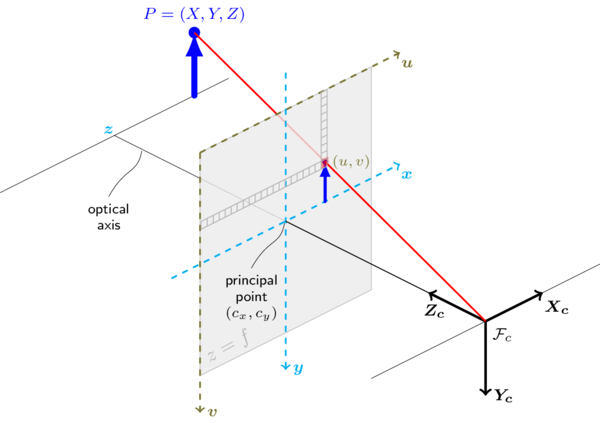
\includegraphics[width = 1.0\hsize]{figures/pinhole_camera_model.png}
	\caption{Pinhole Camera Model}
	\label{pinhole_model}
\end{figure}

Once an object or a point is detected in an image, it is important to transform it into the world frame; to track and gain a 3d appreciation of the environment. For visual understanding and context  of the problem see the pinhole camera model in Figure \ref{pinhole_model}. The only difference, in practice, in an intermediate un-distorting step to get the point's ray. This is due to the focal lens in the camera, which is not represented in the pinhole model but Equation \ref{raddis} shows how to account for this. Hence to find a ray describing a 3d point, the image must first be scaled, (Equation \ref{camera_scale})


\begin{equation}
\begin{aligned}
\mathbf{x''} = \mathbf{k^{-1}(u)} = 
\begin{bmatrix}
\frac{1}{f_{1}} & 0 \\[0.3em]
0 & \frac{1}{f_{2}}
\end{bmatrix}
\bigg (
\mathbf{u} -
\begin{bmatrix}
c_{1} \\[0.3em]
c_{2}
\end{bmatrix}
\bigg )
\end{aligned}
\label{camera_scale}
\end{equation}

where $f_{1},f_{2}$ are x/y focal lengths in pixels, and $c_{1},c_{2}$ is the principal point (image centre) in pixels. The point can be projected to its undistorted location using the reverse of Equation \ref{raddis}.

\begin{equation}
\mathbf{x'} = \mathbf{d^{-1}(x'')}
\label{camera_scale2}
\end{equation}

and finally the ray is calculated by remembering that the z component is of length 1.

\begin{equation}
\mathbf{x} = 
\begin{bmatrix}
\mathbf{x'} \\
1
\end{bmatrix}
\label{to_3d_ray}
\end{equation}

\subsubsection{Calculating the 3D Location}

Now that the ray has been determined we have a point on the 3D unit plane of $z=1$. To find the 3D point in the camera frame, a depth measurement, obtained from the depth camera at the same (undistorted pixel location) is required. Hence the final 3D point is:

\begin{equation}
\mathbf{x} = 
\begin{bmatrix}
\mathbf{x'} \times depth(\mathbf{x'})\\
depth(\mathbf{x'})
\end{bmatrix}
\label{camera_add_depth}
\end{equation}

Assuming a static camera location, this would be all that is needed to map the space in-front of the camera. However, as the camera moves, the origin, and orientation of the camera frame changes with respect to the world frame. Hence the software must not only determine the 3D location of a point in the camera frame but also translate that to a world frame representation.

\subsection{Projecting to World Frame}


\noindent \begin{figure}[h!]
	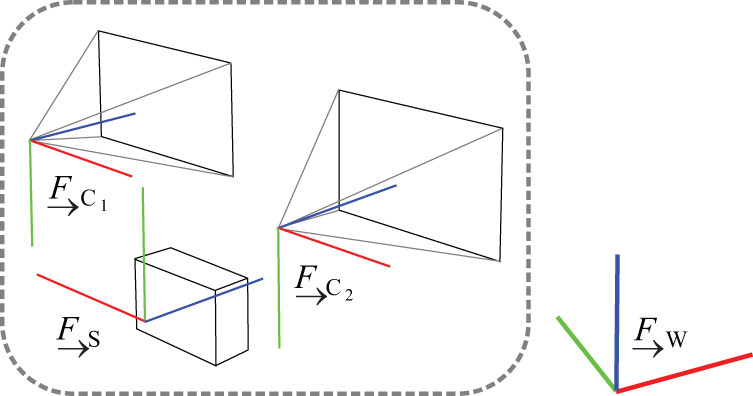
\includegraphics[width = 0.5\hsize]{figures/world_to_cam.jpg}
	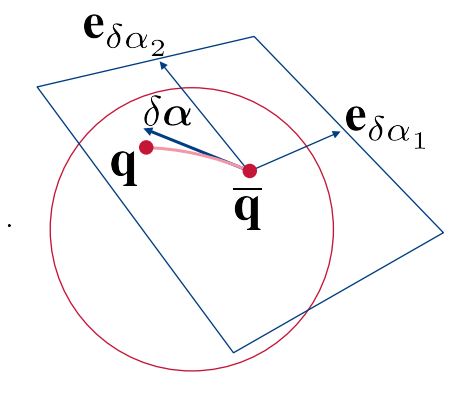
\includegraphics[width = 0.35\hsize]{figures/quaternions.png}
	\caption{World vs Camera Frame (left)\cite{Okvis_1}, Hamiltonian Quaternion (right)}
	\label{quat_wcs}
\end{figure}


To convert between world (${\xrightarrow{F}}_{W}$), camera frame (${\xrightarrow{F}}_{C_{i}}$), and IMU frame (${\xrightarrow{F}}_{S}$), an appropriate method of describing the orientation and location of an object in 3D space is needed. A Hamiltonian Quaternion is capable of correctly mapping the orientation of an object in 3D space, it does this by use of a 4D representation of one real part, and 3 imaginary parts;  

\begin{equation}
\begin{aligned}
\label{quaternion}
q = q_{w} + q_{x}i + q_{y}j+q_{z}k, \\
i^{2}=j^{2}=k^{2}=ijk=-1
\end{aligned}
\end{equation}

With this extra representation of orientation it is possible to map the camera frame to the world frame. Given a position vector in the camera frame $p_{c} = [x,y,z,1]$, it can be converted as follows:


\begin{equation}
\begin{aligned}
T_{WC} = T_{WS} \cdot T_{SC} \\
p_{W} = T_{WC} \cdot p_{C} \\
\end{aligned}
\label{matmul_w2c}
\end{equation}

A transformation between frames is represented as $\textbf{T}_{BA}$ where B and A represent reference frames, so $\textbf{T}_{WC}$ converts between the world frame and camera frame. It is composed of a position and orientation transformation:

\begin{equation}
\begin{aligned}
T_{WC} = 
\begin{bmatrix}
C_{WC} & r_{WC} \\
0_{1 \times 3} & 1
\end{bmatrix}
\end{aligned}
\end{equation}

where $T_{WC} \in \mathbb{R}^{4 \times 4}$, the position translation matrix $r_{WC} \in \mathbb{R}^{3 \times 1}$, and the orientation matrix $C_{WC} \in \mathbb{R}^{3 \times 3}$. Note also that the inverse of this matrix can be easily calculated as $C_{WC}$ is symmetric and therefore positive definite and it holds that $C_{CW}=C_{WC}^{-1}= C_{WC}^{T}$.Therefore:

\begin{equation}
\begin{aligned}
T_{CW} = T_{WC}^{-1} = 
\begin{bmatrix}
C_{WC}^{T} & -C_{WC}^{T}r_{WC} \\
0_{1 \times 3} & 1
\end{bmatrix}
\end{aligned}
\label{invert_tmatrix}
\end{equation}

These transformation matrices must be determined from a SLAM algorithm such as OKVIS which is discussed in the following sections.

\subsubsection{Camera to World Summary}

\begin{algorithm}
	\DontPrintSemicolon
	\SetAlgoLined
	\setstretch{1.3}
	\SetKwInOut{Input}{Input}
	\SetKwInOut{Output}{Output}
	\underline{cam2world} $(cameraPoints,focalMatrix,imageCentre,T_{ws},T_{sc},cameraModel)$\;
	\Input{ \texttt{\\}
		$\mathit{cameraPoints}$ \tcp*[r]{$N$ points in the camera frame $\in R^{3 \times N}$}
		$\mathit{focalMatrix},\mathit{imageCentre}$ \tcp*[r]{Focal Length Matrix, Principal Points [x,y]}
		$\mathit{T_{ws}},\mathit{T_{sc}}$ \tcp*[r]{IMU to World/Camera Matrix}
		$cameraModel$ \tcp*[r]{Camera Model $\in  R^{4 \times 4}$}
	}
	\Output{$N$ points in the world frame $worldPoints \in \mathbb{R}^{3,N}$}
	
	\texttt{\\}
	$x = \mathit{scale\text{\textunderscore}point(imageCentre,focalMatrix,cameraPoints)}$ \tcc*[r]{\text{Equation (\ref{camera_scale})}}
	$x = \mathit{undistort(cameraModel,x)}$ \tcc*[r]{Equation (\ref{raddis})}
	$T_{wc} = matrix\text{\textunderscore}multiply(T_{ws},T_{sc})$
	\texttt{\\}
	$x = \mathit{add\text{\textunderscore}depth(depth,x)}$ \tcc*[r]{Equation (\ref{camera_add_depth}), and Vstack [depth,1] to bottom of x}
	$\mathit{worldPoints} = \mathit{transform\text{\textunderscore}to\text{\textunderscore}world(T_{wc},x)}$ \tcc*[r]{Equation (\ref{matmul_w2c})}
	\texttt{\\}
	\caption{Algorithm to transform camera point to world frame}
	\label{alg:weights}
\end{algorithm}

\subsection{World to Camera Frame} \label{w_c_frame}

In order to correctly plot the Kalman filter and give other tracking algorithms the expected location on the picture, the ability to transform from world to camera frame is needed. The process is similar to the camera to frame except the reverse, namely:

\begin{algorithm}[H]
	\DontPrintSemicolon
	\SetAlgoLined
	\setstretch{1.3}
	\SetKwInOut{Input}{Input}
	\SetKwInOut{Output}{Output}
	\underline{world2cam} $(worldPoints,focalMatrix,imageCentre,T_{ws},T_{sc},cameraModel)$\;
	\Input{ \texttt{\\}
		$\mathit{worldPoints}$ \tcp*[r]{$N$ points in the camera frame $\in R^{3 \times N}$}
		$\mathit{focalMatrix},\mathit{imageCentre}$ \tcp*[r]{Focal Length Matrix, Principal Points [x,y]}
		$\mathit{T_{ws}},\mathit{T_{sc}}$ \tcp*[r]{IMU to World/Camera Matrix}
		$cameraModel$ \tcp*[r]{Camera Model $\in  R^{4 \times 4}$}
	}
	\Output{$N$ points in the camera frame $cameraPoints \in \mathbb{R}^{3,N}$}
	
	\texttt{\\}
	$T_{wc} = matrix\text{\textunderscore}multiply(T_{ws},T_{sc})$
	\texttt{\\}
	$T_{cw} = inverse(T_{wc})$ \tcc*[r]{Equation (\ref{invert_tmatrix})}
	$\mathit{x} = \mathit{transform\text{\textunderscore}to\text{\textunderscore}camera(T_{cw},worldPoints)}$ \tcc*[r]{Equation (\ref{matmul_w2c})}
	$x = \mathit{distort(cameraModel,x)}$ \tcc*[r]{Equation (\ref{raddis})}
	$x = \mathit{remove\text{\textunderscore}depth(depth,x)}$ \tcc*[r]{Reverse Equation (\ref{camera_add_depth})}
	$cameraPoints = \mathit{scale\text{\textunderscore}point(imageCentre,focalMatrix,x)}$ \tcc*[r]{\text{Equation (\ref{camera_scale})}}
	
	\texttt{\\}
	\texttt{\\}
	\caption{Algorithm to transform world point to camera frame}
	\label{alg:weights}
\end{algorithm}


\subsection{Bicycle States}

In order to find the bike location and orientation in each frame; a complete representation of the bike's state is needed. At each taken image ($k$) the bike can be assumed to have a set state $\mathcal{X}_{R}^{k}$. Contained within $\mathcal{X}_{R}$ are a set of pose states, $\mathcal{X}_{T}$, and speed/bias states $\mathcal{X}_{sb}$, Equation \ref{states_1}. Landmarks are contained within the set $\mathcal{X}_{L}$.

\begin{equation}
\begin{aligned}
\label{states_1}
\mathcal{X}_{T} := [ _{W}r_{S}^{T},q_{WS}^{T} ]^{T} \\
\mathcal{X}_{sb} := [ _{s}v^{T},b_{g}^{T}, b_{a}^{T} ]^{T} \\
\mathcal{X}_{R} := [ _{W}r_{S}^{T},q_{WS}^{T},_{s}v^{T},b_{g}^{T}, b_{a}^{T}]^{T}
\end{aligned}
\end{equation}

The elements $_{W}\textbf{r}_{S}^{T}$, $\textbf{{q}}_{W}^{T}$ are the position and the quaternion body orientation, $_{s}\textbf{{v}}^{T}$ the velocity, $\textbf{{b}}_{g}$ \& $\textbf{{b}}_{a}$ the accelerometer and gyroscope biases.


\subsection{The SLAM Problem}

If measurements were exact, mapping of an environment would be easy. This, however is not the case, there is often noise associated with each taken measurement and movement. For example distance measurements and IMU readings are subject both to a noise and a bias (calibration error) which can both be assumed to be Gaussian distributed.

\begin{equation}
\begin{aligned}
\mathbf{\tilde{z}} = \textbf{b}_{c} + s\textbf{M}_{z} + \textbf{b} + \textbf{n} + \textbf{o}
\end{aligned}
\label{measurement_model}
\end{equation}

where $\textbf{z}$ is the correct measurement, $\textbf{b}_{c}$ is a long-term constant bias, $s$ is a scaling factor, $\textbf{M}$ - misalignment, $\textbf{b}$ - time varying bias, $n$ - noise, and $o$ contains other un-modelled influences. This means that no measurement can be trusted exclusively for state-space information. \newline\newline
Historically, before the recent advances in SLAM, it was first assumed that errors have a compounding effect. The position of a bike, would become increasingly unknown as the environment is explored and the bike is displaced from the origin. This makes intuitive sense if say there is only IMU measurements available. At each step, more uncertainty is introduced from the noise and biases (shown in Equation \ref{measurement_model}) and the bike's position becomes more and more uncertain. 
\newline \newline
For some time it was also presumed to be the case even when external measurements of the environment are taken. This, however, is not the case as proved by Durrant-Whyte \cite{F_Durr_1} since there is a high degree of correlation between estimates of different landmarks and locations in a map, these correlations also increase with successive observations (Figure \ref{slam_prob_fig}). As an example of this (Figure \ref{slam_prob_fig} : Right) displays error in measurements of landmark observation, the mean error is common between all landmarks and so with successive landmark observations, the errors in location estimates become highly correlated. This means that although $\textbf{m}_{i}$'s location may be quite uncertain but the relative location between two landmarks $\textbf{m}_{i}-\textbf{m}_{j}$ is well-known.\newline

In the case of the bicycle set-up, there is both an IMU, and a camera. These provide the basic inputs to the OKVIS software \cite{Okvis_1}. Okvis is able to determine the bike's location by optimising the total error, hence combining both the camera and IMU error.

\noindent \begin{figure}[h!]
	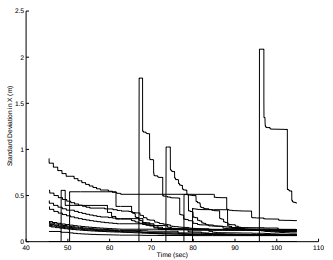
\includegraphics[width = 0.5\hsize]{figures/convergence_landmark_uncertainty.png}
	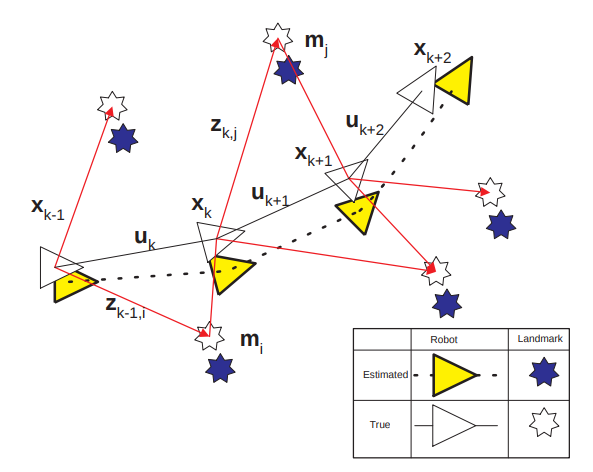
\includegraphics[width = 0.5\hsize]{figures/ess_slam.png}
	\caption{Left: Convergence in landmark uncertainty.  Over time, standard deviations reduce monotonically to a lower bound \cite{F_Durr_Pt1}. Right: Error between estimated and true landmarks is common.}
	\label{slam_prob_fig}
\end{figure}


\subsubsection{Batch NonLinear Least Squares}

Given an error function for the camera and IMU in the form:

\begin{equation}
\begin{aligned}
J(\mathbf{x}) := \frac{1}{2} \sum_{n=1}^{N} \textbf{e}_{n} (\textbf{x})^{T} \textbf{W}_{n} \textbf{e}_{n}(\textbf{x}) 
\end{aligned}
\end{equation} 

where $\textbf{e}_{n}(\cdot)$ is an error term that is weighted by $\textbf{W}_{n}$, and would consist, in this case of the camera and IMU error. The only way to minimise this error is through observations which are also presumed to have an associated noise term.

\begin{equation}
\begin{aligned}
\textbf{z}_{n} = g_{n}(\textbf{x}) + \textbf{v}_{n},
\end{aligned}
\end{equation} 

where $z_{n}$ is the observation, $g_{n}(\textbf{x})$ the observation model, and $v_{n} ~ \mathcal{N}(0,Q_{n})$ and are independent. Hence as $v_{n}$ is mean 0, the error can be simply formulated by:

\begin{equation}
\textbf{e}_{n}(\textbf{x}) = z_{n} - g_{n}(\textbf{x})
\end{equation}
\begin{equation}
\mathit{error = observation - predicted \textnormal{ } observation}
\end{equation}

Since observation noise between the IMU and camera $v_{n}$ are independent the covariance matrix is diagonal. Hence $W_{n} = E[\mathbf{e}_{n} \mathbf{e}_{n}^{T}]^{-1} = Q^{-1}$. The aim of least squares is to find the state vector $\mathbf{x}$ that minimises the error function, hence the optimisation problem is posed as:

\begin{equation}
\begin{aligned}
\textbf{x} = argmin(J(\mathbf{x}))
\end{aligned}
\end{equation}

If the error term $\mathbf{e}_{n}(\mathbf{x})$ was linear w.r.t $\mathbf{x}$ the solution would be a simple as setting the $\frac{\delta J(\mathbf{x})^{T}}{\delta \mathbf{x}}$ to zero and solving the respective simultaneous equations. However this is often not the case, and so the solution to the equation must be solved iteratively, with for example, gauss-newton formulation of the equations and a solver such as google-ceres.

\subsection{Frame to Frame Matching}\label{BRISK_section}

\paragraph{Keypoint Detection}

The Okvis \cite{Okvis_1} paper uses an corner detection method to determine keypoints and then matches these keypoints using a binary descriptor (BRISK \cite{BRISK}). In the BRISK paper a modification of the FAST feature extractor is used, however, in the OKVIS implementation a modified Harris Corner detection algorithm is utilised. A simplistic way to think of this is how one would go about determining a corner in an image. Imagine an edge, it is simply a location on an image where the brightness gradient changes rapidly in one direction (perpendicular to the edge). Hence a corner is a similar change but in two such directions. Imagine a location $(x,y)$ and a small displacement from that location $(x+ \Delta x, y + \Delta y)$. An area of rapid gradient change would have very different intensity values at $(x,y)$ and surrounding points. Hence a corner will maximise the sum of squared differences between points.

\begin{equation}
\begin{aligned}
f(x,y) = \sum_{x_{k},y_{k} \in W} (I(x_{k},y_{k}) - I(x_{k} + \Delta x,y_{k} + \Delta y))^{2}
\end{aligned}
\end{equation}

This can be further distilled by the Taylor expansion to:

\begin{equation}
\begin{aligned}
f(x,y) = \sum_{(x,y)\in W} (I_{x}(x,y) \Delta x + I_{y}(x,y) \Delta y )^{2}
\end{aligned}
\end{equation}

or in matrix form:

\begin{equation}
M = 
\begin{bmatrix}
\sum_{(x,y) \in W} I_{x}^{2} & \sum_{(x,y) \in W} I_{x}I_{y} \\
\sum_{(x,y)\in W} I_{x}I_{y}& 
\sum_{(x,y)\in W} I_{y}^{2}
\end{bmatrix} = 
R^{T}
\begin{bmatrix}
\lambda_{1} & 0 \\
0 & \lambda_{2}
\end{bmatrix}
R
\end{equation}
\begin{equation}
f(x,y) = (\Delta x \textnormal{ } \Delta y) M 
\begin{bmatrix}
\Delta \mathbf{x} \\
\Delta \mathbf{y}
\end{bmatrix}
\end{equation}

where M is the structure tensor (also commonly known as the Second Moment Matrix). The Harris corner response then is taken from the eigenvalues of M, intuitively since the gradient changes rapidly the second moment matrix eigenvalues are large in that direction Figure \ref{Harris}.


\begin{equation}
\begin{aligned}
R = det(M) - \mathit{k}trace(M)^{2} = \lambda_{1}\lambda_{2} - \mathit{k}(\lambda_{1} + \lambda_{2})^{2}
\end{aligned}
\end{equation}

\noindent \begin{figure}[H] 
	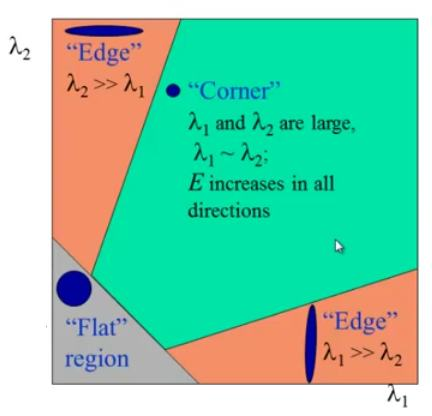
\includegraphics[width = 0.5\hsize]{figures/harris_region.jpg}
	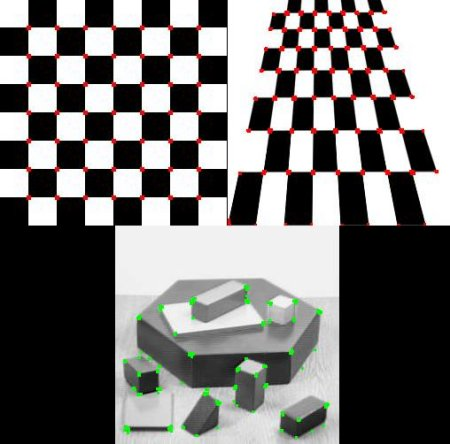
\includegraphics[width = 0.45\hsize]{figures/harris_result.jpg}
	\caption{Left: Structure Tensor Eigenvalues, Right: Harris corner detection result \cite{opencv_harris_article} }
	\label{Harris}
\end{figure}

\paragraph{Keypoint Matching}
Binary descriptors use a sampling pattern to create pairs of points (lines). The algorithm then compares the two points ($p1,p2$) and if $p1 > p2$ a 1 is recorded and otherwise 0. This creates a binary string, that along with orientation representation describe a keypoint. When matching keypoints between images a simple, and fast $\sum XOR$ reveals keypoint similarity from which a threshold can be used to determine matches.

\noindent \begin{figure}[H] 
	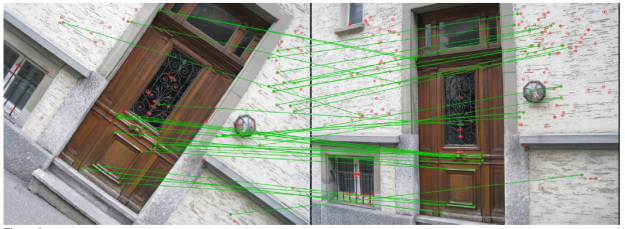
\includegraphics[width = 0.7\hsize]{figures/brisk.jpg}
	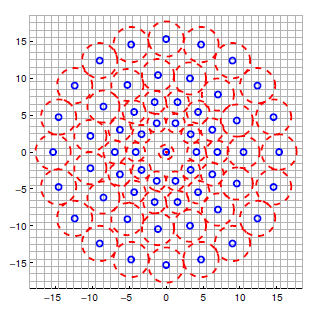
\includegraphics[width = 0.26\hsize]{figures/brisk.png}
	\caption{Left: Brisk keypoint matching example, Right: Brisk Sampling Pattern \cite{BRISK} }
	\label{Brisk}
\end{figure}

The BRISK sampling pattern (Figure \ref{Brisk}: Right) uses a standard Gaussian smoothing at each sample point. The standard deviation of the sample is represented by the red circles in the figure. This ensures the sample is less prone to noise than other traditional binary detectors e.g. BRIEF.



\subsubsection{Camera Re-projection Error}

As discussed in Section \ref{w_c_frame}, the camera uses a lens to take a photograph. This, especially on cheaper cameras, can distort the image. The distortion is intrinsic to the camera and it needs to calibrated to determine a distortion model $\mathbf{d}(^{.})$. This is then used to determine the re-projection error \cite{Furgale}.

\begin{equation}
\begin{aligned}
\textbf{e}_{r}^{i,j,k} = \textbf{z}^{i,j,k} - \textbf{d}_{i} (\textbf{T}^{k}_{CiS} \textnormal{ } \textbf{T}^{k}_{SW} \textnormal{ } _{w}\textbf{l}^{j})
\end{aligned}
\end{equation}

where $\textbf{z}^{i,j,k}$ denotes the measurement image coordinates.

\subsubsection{IMU Kinematics}

Therefore the kinematics of the IMU can be modelled as:

\begin{equation}
\label{imu_kin}
_{W} \textbf{\.{r}}_{S} = \textbf{C}_{WS} \textnormal{ } _{s}\textbf{v}
\end{equation}
\begin{equation}
\textbf{\.{q}}_{WS} = \frac{1}{2} \Omega(\tilde{_{S}\textbf{$\omega$}})\textbf{q}_{WS}
\end{equation}
\begin{equation}
_{S}\textbf{\.{v}}= (_{S}\tilde{\textbf{a}} + \textbf{w}_{a} - \textbf{b}_{a}) + C_{SW} \textnormal{ } _{W}\textbf{g} - (_{S}\textbf{$\omega$}) \times _{S}\textbf{v}
\end{equation}
\begin{equation}
\textbf{\.{b}}_{g} = \textbf{w}_{bg}
\end{equation}
\begin{equation}
\textbf{\.{b}}_{a} = -\frac{1}{\tau}\textbf{b}_{a} + \textbf{w}_{ba}
\end{equation}

where:
\begin{equation}
\Omega(\tilde{_{s}\textbf{$\omega$}}) = \begin{bmatrix}
-_{S}\textbf{$\omega$}  \\[0.3em]
0
\end{bmatrix} ^{\oplus}
\end{equation}
\begin{equation}
_{S}\textbf{$\omega$} =  _{S}\tilde{\textbf{$\omega$}} + \textbf{w}_{g} - \textbf{b}_{g}
\end{equation}

$_{W} \textbf{\.{r}}_{S}$ represents the position derivative likewise $_{S}\textbf{\.{v}}$ for velocity,  $_{S}\tilde{\textbf{a}}$ accelerometer measurements, $_{W}\textbf{g}$ earth's gravitational acceleration vector, and finally w:= [$w_{g}^{T},w_{a}^{T},w_{bg}^{T},w_{ba}^{T}$] are independent Gaussian white noise processes with zero mean.

\subsubsection{IMU Kinematics Linearised}

In order to optimise the cost function, it is important to linearise the IMU kinematics. The error dynamics take the form:

\begin{equation}
\begin{aligned}
\delta \mathcal{X} \approx  \textbf{F}_{c} (\overline{x}_{R}) \delta \mathcal{X}_{R} + \textbf{G}(\overline{x}_{R})\textbf{w} \\
\end{aligned}
\end{equation}

\begin{equation}
\begin{bmatrix}
\delta \textbf{\.r}  \\[0.3em]
\delta \textbf{\.a} \\[0.3em]
\delta \textbf{\.v} \\[0.3em]
\delta \textbf{\.b}_{g} \\[0.3em]
\delta \textbf{\.b}_{a}
\end{bmatrix}
=
\begin{bmatrix}
0_{3 \times 3} &  [\overline{C}_{WS}\overline{v}]^{\times}
& \overline{C}_{WS} &  0_{3 \times 3} &  0_{3 \times 3}\\

0_{3 \times 3} & 0_{3 \times 3} 
& 0_{3 \times 3} &  -\overline{C}_{WS} &  0_{3 \times 3}\\

0_{3 \times 3} & -\overline{C}_{WS}[_{W}\textbf{g}]^{\times}
& -[_{S}\overline{\omega}]^{\times} &  -[_{S}\overline{v}]^{\times} &  -I_{3}\\

0_{3 \times 3} & 0_{3 \times 3}
& 0_{3 \times 3} &  0_{3 \times 3} &  0_{3 \times 3}\\

0_{3 \times 3} & 0_{3 \times 3} 
& 0_{3 \times 3} &  0_{3 \times 3} &  -\frac{1}{\tau}\textbf{I}_{3}
\end{bmatrix}
\begin{bmatrix}
\delta \textbf{r}  \\[0.3em]
\delta \textbf{a} \\[0.3em]
\delta \textbf{v} \\[0.3em]
\delta \textbf{b}_{g} \\[0.3em]
\delta \textbf{b}_{a}
\end{bmatrix}
+
\begin{bmatrix}
0_{3 \times 3}  \\[0.3em]
\overline{C}_{WS} \textbf{W}_{g} \\[0.3em]
\overline{C}_{WS} \textbf{W}_{a} \\[0.3em]
\textbf{W}_{bg} \\[0.3em]
\textbf{W}_{ba}
\end{bmatrix}
\end{equation}

This formulation of the error dynamics is then used to derive the IMU error term (Equation \ref{imu_error_}), for further details see \cite{Okvis_1}.


\begin{equation}
\mathbf{e}^{k}_{s}(\mathbf{x}^{k}_{R},\mathbf{x}^{k+1}_{R},\mathbf{z}_{s}^{k}) = 
\begin{bmatrix}
_{W} \hat{\mathbf{r}}_{S}^{k+1} - _{W}\mathbf{r}_{S}^{k+1} \\

2[\hat{\mathbf{q}}_{WS}^{k+1} \otimes \mathbf{q}_{WS}^{k+1 \textnormal{ } -1]} \\

\hat{\mathbf{x}}^{k+1}_{sb} - \mathbf{x}_{sb}^{k+1}
\end{bmatrix}
\label{imu_error_}
\end{equation}

\section{Background Object Tracking}

Object tracking has been recently advanced by means of discriminative learning methods, these methods try to distinguish between the object and the environment that it is in. The model must therefore be fed negative samples to understand the relevant environment. 

\subsection{Kernelised Correlation Filter} \label{kcf_background}

In the recent paper by Henriques et al. \cite{kcf} the tools are developed to supply thousands of negative samples without iterating over them explicitly. The paper makes use of circulant matrices to provide negative samples. These are obtained by translating the data using a \textit{cyclic shift operator}, which in the 1D signal case is:

\begin{equation}
P = 
\begin{bmatrix}
0 & 0 & \dots & 0 & 1 \\
1 & 0 & \dots & 0 & 0 \\
0 & 1 & \dots & 0 & 0 \\
\vdots & \vdots & \vdots & \ddots & \vdots \\
0 & 0 & \dots & 1 & 0
\end{bmatrix}
\end{equation} 

Therefore the product of $P\mathbf{x} = [x_{n},x_{1},x_{2},...,x_{n-1}]$ and any shift can be modelled using $P^{u}\mathbf{x}$. Because of its cyclic nature, the signal $\mathbf{x}$ repeats when $u=n$ and so the full set of shifted signals is obtained with ${P^{u}\mathbf{x} | u=0,...,n-1}$. An example of this is shown in the 1D case by Figure \ref{circular_data}.

\noindent \begin{figure}[h!]
	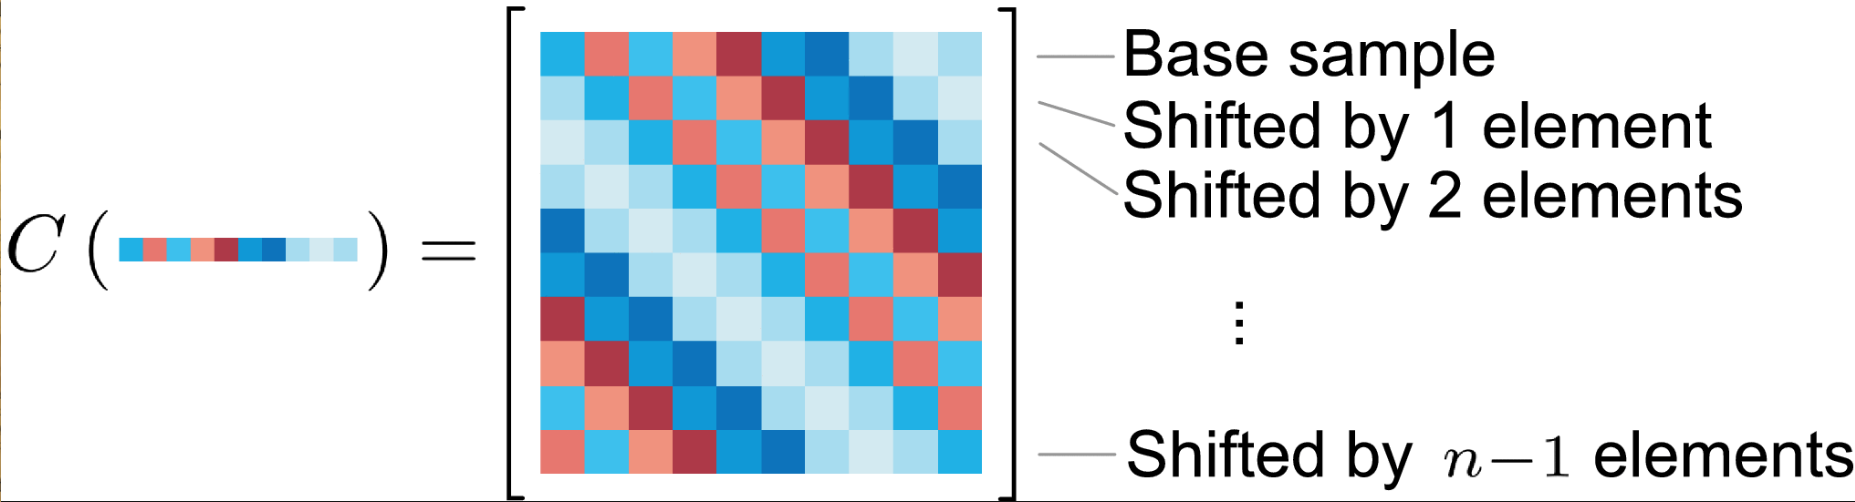
\includegraphics[width = 1.0\hsize]{figures/circular_shift.png}
	\caption{Illustration of circulant matrix.\cite{kcf}}
	\label{circular_data}
\end{figure}

Therefore to compute the regression with shifted samples, the data matrix $X$ takes the form:

\begin{equation}
X = C(\mathbf{x}) = 
\begin{bmatrix}
x_{1} & x_{2} & \dots & x_{n-1} & x_{n} \\
x_{n} & x_{1} & \dots & x_{n-2}  & x_{n-1}  \\
x_{n-1} & x_{n} & \dots & x_{n-3} & x_{n-2}  \\
\vdots & \vdots & \vdots & \ddots & \vdots \\
x_{2}  & x_{3}  & \dots & x_{n} & x_{1} \\
\end{bmatrix}
\end{equation}

Noting that all circulant matrices can be diagonalised by the Discrete Fourier Transform (DFT) $X$ can be written as:


\begin{equation}
\mathit{F}(\mathbf{z}) = \sqrt{n}F\mathbf{z}
\end{equation}
\begin{equation}
\hat{\mathbf{x}} = \mathit{F}(\mathbf{x})
\end{equation}
\begin{equation}
X = F diag(\hat{\mathbf{x}}) F^{H}
\end{equation}

This is possible because the DFT is a linear operation. 

\subsubsection{Kernels}\label{kcf_kernels}

Using a kernel, the model can implicitly use a high-dimensional feature space. The kernel function used to do this (e.g. Gaussian), Equation \ref{gauss_kernel} creates an $n \times n$ kernel matrix $K_{i,j} = k(\mathbf{x}_{i},\mathbf{x}_{j})$

\begin{equation}
k(\mathbf{x},\mathbf{x}') = exp (\frac{1}{\sigma^{2}} ||\mathbf{x} - \mathbf{x}'||^{2})
\label{gauss_kernel}
\end{equation}

and therefore the function becomes:

\begin{equation}
f(\mathbf{z}) = \mathbf{w}^{T}\mathbf{z} = \sum_{i=1}^{n} \alpha_{i}k(\mathbf{z},\mathbf{x}_{i})
\end{equation}

with the solution of kernelised Ridge Regression given by:

\begin{equation}
\mathbf{\alpha} = (K + \lambda I)^{-1} \mathbf{y}
\label{kernel_soln}
\end{equation}

where $K$ is the kernel matrix and $\mathbf{\alpha}$ is the vector of coefficients $\alpha_{i}$. Given a kernel function that combines data through a commutative operation, it can be proven that given circulant data the kernel matrix $K$ is also circulant and therefore the DFT trick can be used. This leads to a diagonalisation of Equation \ref{kernel_soln} to Equation \ref{al_soln}.

\begin{equation}
\mathbf{\hat{\alpha}} = \frac{\mathbf{\hat{y}}}{\mathbf{\hat{k}}^{\mathbf{xx}} + \lambda}
\label{al_soln}
\end{equation}

where $\mathbf{\hat{k}}^{\mathbf{xx}}$ is the first row of the kernel matrix $K = C(\mathbf{\hat{k}}^{\mathbf{xx}})$, and a $\hat{ }$ denotes the DFT of a vector. This means that only an $n \times 1$ kernel matrix needs to be computed, due to the circulant kernel property and DFT. This makes the method far faster than conventional kernel methods that require an $n \times n$ sized kernel matrix.


\subsubsection{Detection}

The basic premise is that the $\alpha$ term in Equation \ref{al_soln} is now initialised to a learnt set of coefficients that correctly describe the object. Therefore, in order to detect the object of interest the regression function $f(\mathbf{z})$ must be evaluated at a number of candidate patches.  These patches can themselves also be described by circulant shifts. Defining the kernel matrix $K^{z}$ between cyclic shifts of base samples $x$ and $z$, with elements $k(P^{i-1}z,P^{j-1}x)$. The cyclic property, as described in Section \ref{kcf_kernels} allows only the first row of the kernel matrix to be relevant, and hence :

\begin{equation}
K^{z} = C(\mathbf{k^{xz}})
\end{equation}

where $k^{xz}$ is the kernel correlation of $x$ and $z$. Finally the regression equation can be computed for all candidate patches by:

\begin{equation}
f(z) = (K^{z})^{T} \alpha
\end{equation}

This can be further sped up by the correct choice of kernel function and a clever kernel trick to modify the computational cost of kernel computation to $O(nlogn)$. 

%%%%%%%%%%%%%%%%%%%%%%%%%%%%%%%%%%%%
\chapter{Contribution}


\section{Software Solution}
The system consists of a number of modules, each responsible for a specific aspect see Figure \ref{software_soln} for more details. These will now be summarised below, then a more in-depth review will occur in upcoming sections of the report. The realsense camera feeds data into three modules, Okvis for SLAM and a global representation of the environment, the cyclist model for path prediction and finally Mask-RCNN to segment the image and detect objects in the camera frame. Okvis also provides information into the cyclist model which needs to understand the bike's location in the world frame to predict future positions.

\noindent \begin{figure}[h!]
	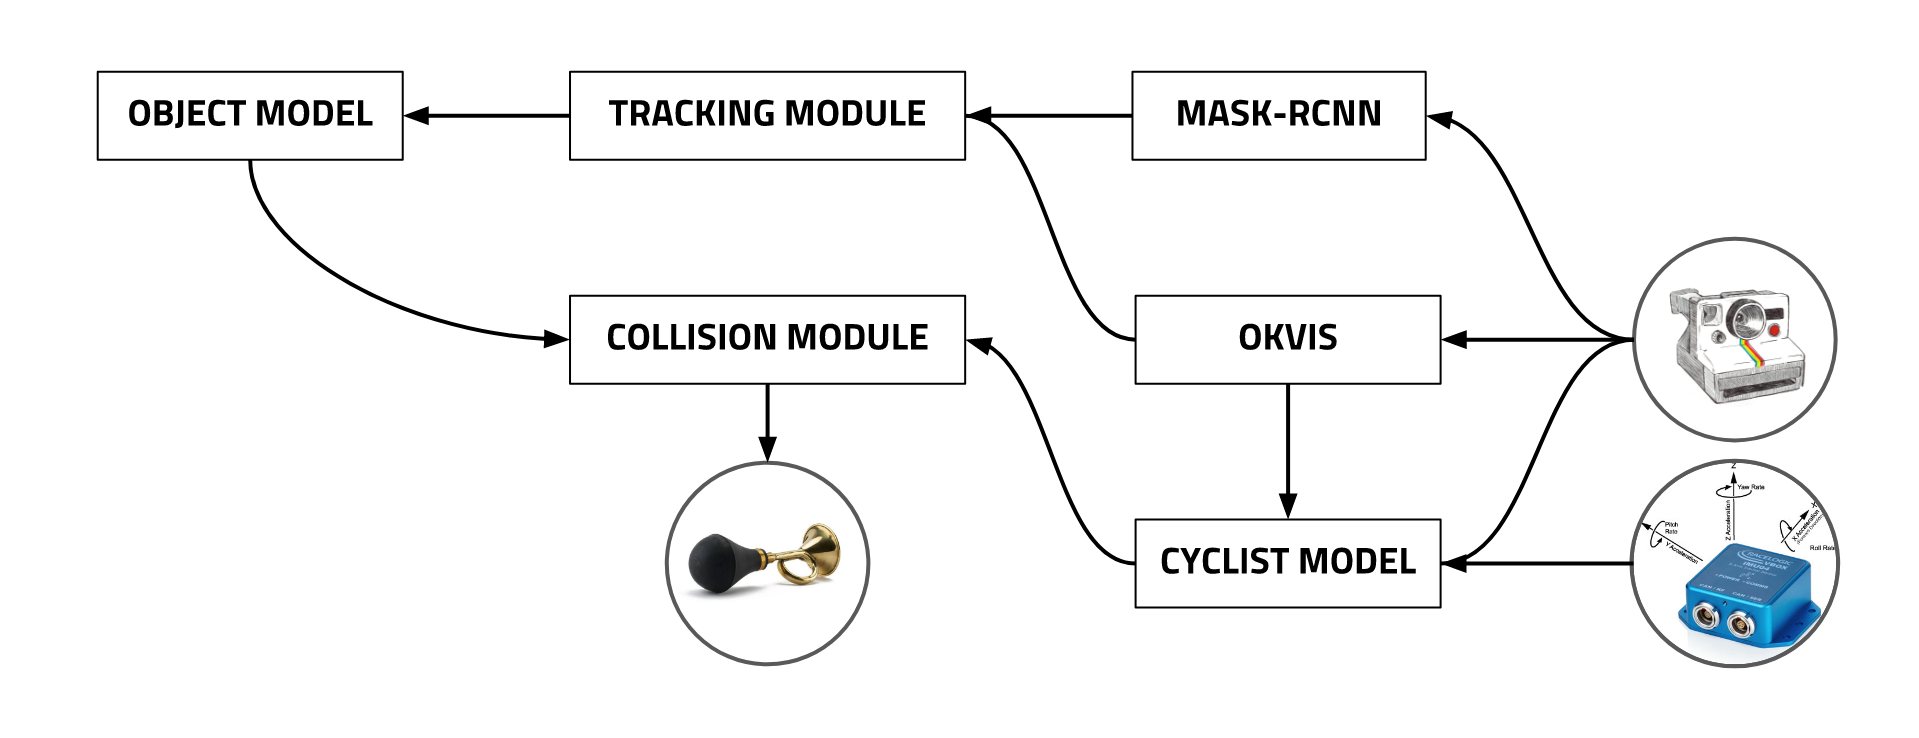
\includegraphics[width = 1.0\hsize]{figures/software_architecture.png}
	\caption{System Design}
	\label{software_soln}
\end{figure}

\paragraph{Tracking Module}

The tracking module takes the segmented image masks from Mask-RCNN, the passed-on depth image and Okvis pose output to determine the location of a detected object. The distance of an object is inferred from the depth camera, and masks which can then be converted into the world frame using the Okvis pose. From these outputs and a passed image, various features from objects can be matched from frame-to-frame. These features include global position, BRISK keypoints, and the KCF model of the object. Once the objects from the previous frame are correctly identified and new object added the object model can begin to predict an object's future movement.

\paragraph{Collision Module}
The collision module takes predicted positions from the object models and cyclist models. It then determines whether there is a large likelihood of intersection between the cyclist and objects in the future. The idea of this is to then notify both the object (possibly a person or car) that they are about to collide and the cyclist, hopefully both parties, once aware of the unfolding situation can take preventive measures to avoid eachother.

\paragraph{Limitations}
Sadly the system currently cannot run in realtime due to Mask-RCNN, the current state of the art segmentation network taking c. 0.5s to predict an image. There is a future possibility of incorporating a simpler, and faster network such as YOLO which foregoes the advantage of segmentation (useful for depth approximation) but would run in real-time.


\section{Depth Measurement Outlier Removal} \label{Depth_approx}

In order to get the depth measurement of an object, the mask output from Mask R-CNN is overlayed onto the depth map and a mean depth is taken. A number of points are not detected and therefore large quantities of the depth map is 0. Therefore, the median depth is selected only from coordinates at which $depth>0$. Figure \ref{DCO} shows some examples of a depth camera image taken in the Imperial Library.

\noindent \begin{figure}[h!]
	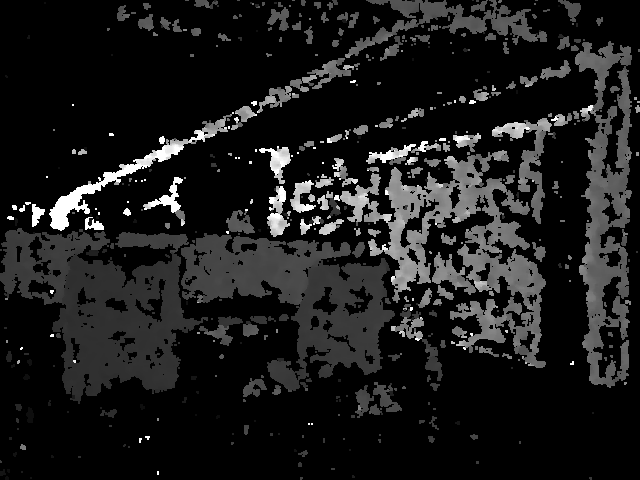
\includegraphics[width = 0.5\hsize]{figures/depth_image_1.png}
	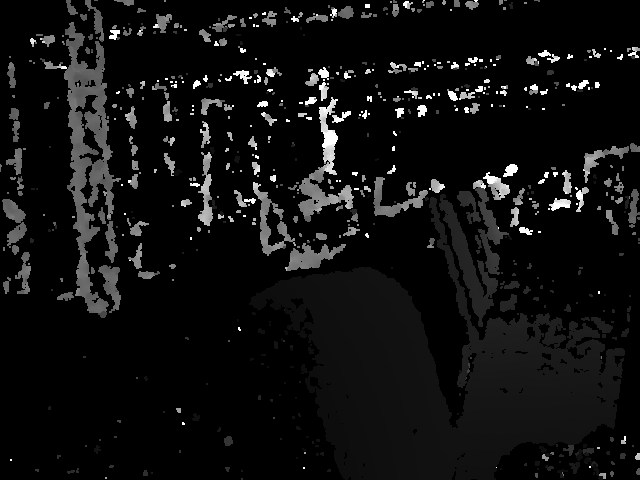
\includegraphics[width = 0.5\hsize]{figures/depth_image_2.png}
	\caption{Depth Camera Output}
	\label{DCO}
\end{figure}

As can be seen from Figure \ref{DCO} the data is sparse and unreliable for objects at a distance. This is less so as the depth is scaled [0-255] for a picture and so some measurements seem less reliable than they are but it is still a challenge. Often when the depth measurements are incorrect an unfeasibly large value is returned > 50m. This is a real problem for tracking objects, not necessarily after a period of successful tracking as the value can be discarded as an outlier but on initialisation or after only a couple of data points. Not only is the depth incorrect but that problem is in both x and y when transformed to the world frame. Am example of this phenomenon is displayed in Figure \ref{bottle} where a bottle is tracked from frame to frame, which also demonstrates the ability of the tracking method to be non-cycling domain specific.

\noindent \begin{figure}[h!]
	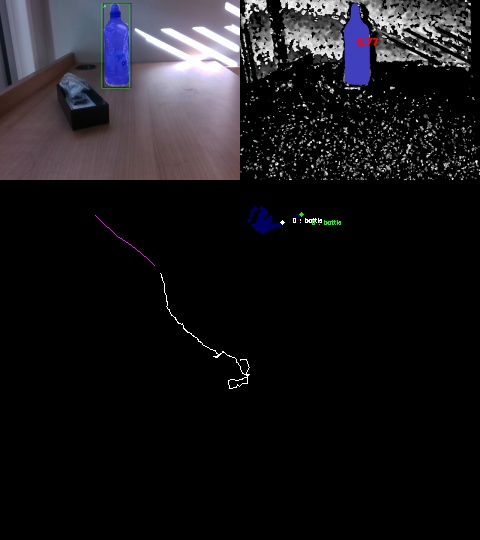
\includegraphics[width = 0.5\hsize]{figures/bottle2.jpg}
	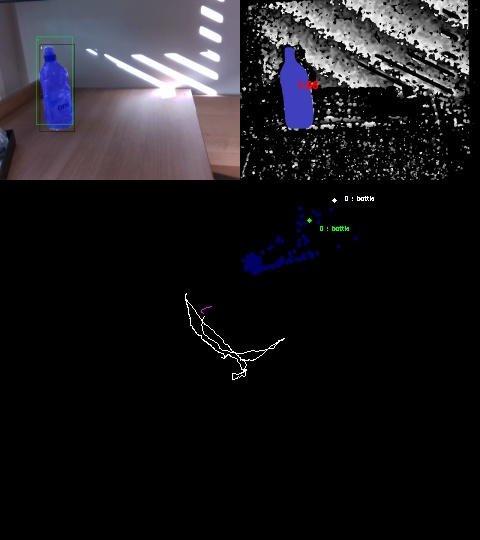
\includegraphics[width = 0.5\hsize]{figures/bottle1.jpg}
	\caption{Left: Bottle with working depth, Right: Incorrect Depth measurement. In both cases the white dot is the bottle's location, the green dot is the Kalman filter prediction, blue dots are previous locations (the bottle did not move), and the white line is the camera location.}
	\label{bottle}
\end{figure}

This can occur in a number of instances and far away objects are most prone as there is little area covered on the depth image to measure the distance from. However, since the object is defined by a bounding box, prior knowledge of the classes can be used to detect such an outlier. Intuitively if two objects are the same size in an image and the first is closer than the second, then the latter object must be larger than the first. Hence using the camera to world model, if the depth is incorrectly large the height of the object in the world frame will be far larger than is known to be possible i.e. a 10m tall human.

Given the knowledge that human sizes roughly vary from a 4ft child to a 7ft adult, poor depth predictions convert people to outside of that range. If that is the case then it must be modified to an approximate value, say the depth of an averagely sized human $1.5m$. This logic can be extended to other objects such as cars and bikes. Therefore, assuming a bounding box of $[x_{tl},y_{tl},x_{br},y_{br}]$, where $tl$ denotes top-left corner and $br$ is the bottom right, the matrix P can be formed.

\begin{equation}
\mathbf{P} = 
\begin{bmatrix}
x_{tl} & x_{tl}\\
y_{tl} & y_{br} \\
\end{bmatrix}
\label{check__depth_eq1}
\end{equation}

Completing the initial steps of Cam2World (Section \ref{cam2world}) until Equation \ref{camera_add_depth}, and adding the 1 required for the proceeding transform, the process yields:

\begin{equation}
\mathbf{K} = 
\begin{bmatrix}
k_{(1,1)}\mathit{d} & k_{(1,2)}\mathit{d}\\
k_{(2,1)}\mathit{d} & k_{(2,2)}\mathit{d}\\
\mathit{d} & \mathit{d}\\
1 & 1
\end{bmatrix}
\label{check__depth_eq2}
\end{equation}

Where $[k_{(1,1)},k_{(2,1)}]$ are from $[x_{tl},y_{tl}]$, $[k_{(1,2)}, k_{(2,2)}]$  from $[x_{tl},y_{br}]$, and $\mathit{d} = depth(\mathbf{x'})$ from the depth image. For the next steps, the transformation matrix $T_{WC}$ is used to calculate the world position.

\begin{equation}
\mathbf{T_{WC}} = 
\begin{bmatrix}
\dots r_{1} \dots \\
\dots r_{2} \dots \\
\dots r_{3} \dots \\
\dots r_{4} \dots \\
\end{bmatrix}
\label{check__depth_eq2}
\end{equation}

where $r_{i}$ denotes row $i$ of $T_{WC}$, and $r_{4} =[0_{3 \times 1},1]$. Therefore replicating a simple matrix multiplication in Equation \ref{check__depth_eq3}, the row $r_{3}$ is the only row from $\mathbf{T}_{WC}$ that is needed for the object height.

\begin{equation}
\mathbf{WorldPoints} = 
\begin{bmatrix}
x_{w,tl} &  x_{w,bl}\\
y_{w,tl} & y_{w,bl}\\
z_{w,tl} & z_{w,bl} \\
\end{bmatrix} = 
\mathbf{T}_{WC}\mathbf{K} =
\begin{bmatrix}
\dots r_{1} \dots \\
\dots r_{2} \dots \\
\dots r_{3} \dots \\
\dots r_{4} \dots \\
\end{bmatrix}
\begin{bmatrix}
k_{(1,1)}\mathit{d} & k_{(1,2)}\mathit{d}\\
k_{(2,1)}\mathit{d} & k_{(2,2)}\mathit{d}\\
\mathit{d} & \mathit{d}\\
1 & 1
\end{bmatrix} 
\label{check__depth_eq3}
\end{equation}

Hence the height of the object $z_{w,tl}-z_{w,bl}$ is obtained from:

\begin{equation}
\begin{aligned}
z_{w,tl}-z_{w,bl} = r_{3} \mathbf{K}[:,1] - r_{3} \mathbf{K}[:,2] =  r_{3} (\mathbf{K}[:,1]- \mathbf{K}[:,2])
\end{aligned}
\end{equation}

where $\mathbf{K}[:,1]$ defines the first column of K, and defining vector $A$ as:

\begin{equation}
\begin{aligned}
A\mathit{d} = \mathbf{K}[:,1]- \mathbf{K}[:,2] = 
\begin{bmatrix}
k_{(1,1)}\mathit{d} - k_{(1,2)}\mathit{d}\\
k_{(2,1)}\mathit{d} - k_{(2,2)}\mathit{d}\\
0\\
0
\end{bmatrix}
= 
\mathit{d}
\begin{bmatrix}
k_{(1,1)} - k_{(1,2)}\\
k_{(2,1)} - k_{(2,2)}\\
0\\
0
\end{bmatrix}
\end{aligned}
\end{equation}

then an approximation of the depth, given the average object height $o_{av}$ is:

\begin{equation}
\begin{aligned}
depth \approx \frac{o_{av}}{r_{3}A} 
\end{aligned}
\end{equation}

Once this depth approximation is found the relevant models can get a depth update that is approximately correct unlike the actual camera depth measurement. This allows better modelling and tracking of object movement from frame-to-frame.

\section{Tracking Module}

For each frame Mask RCNN outputs a set of bounding boxes, and masks. These are not within any particular order and so a method must be devised to track objects from one frame to the next. This is a hard challenge due to object occlusion, variation in shadow/lighting conditions and rapid in-frame movement. An obvious method is intersection over union (IOU) of the bounding boxes on a frame-by-frame basis. This is good in theory, however, it lacks the ability to compensate for rapid movement (of the object and the camera angle), occlusion and object overlapping. A set of methods have therefore been developed to overcome this problem, which combined provide a robust tracking system.
\newline \newline
The method must both track objects in the frame, determine which objects are no-longer in-frame and find any new objects that enter the frame. Information about each object must be stored as to determine the velocity and direction of travel/ if a collision is likely between the cyclist and the object in question. Figure \ref{roi_match} displays an example of a working system.

\noindent \begin{figure}[h!]
	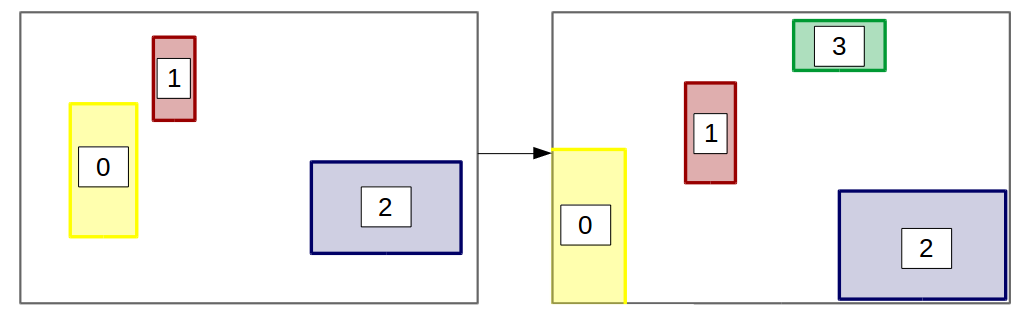
\includegraphics[width = 1.0\hsize]{figures/roi_match.png}
	\caption{RoI Old to New Frame Example.}
	\label{roi_match}
\end{figure}


\subsection{Kernelised Correlation Filter}
A Kernelised correlation filter - one of the state-of-the-art methods used today for tracking objects from one frame to another is described in Section \ref{kcf_background}. A minor modification is required for use in a multi-object scenario which is described below:

\paragraph{Modifications:}
Since the bbox prediction is so fast for the KCF tracker; it can be used in conjunction with the other tracking methods mentioned in Sections \ref{BRISK_matching}, \ref{class_matching}, and \ref{kalman_matching}. The kcf tracking algorithm outputs a bounding box which is the predicted coordinates of the object in the next frame. This can be compared to Mask-RCNNs output through a simple matching process. A box in the new frame predicted by Mask RCNN $[x_{mask}$,$y_{mask}$,$width_{mask}$,$height_{mask}]$ can be scored by sampling the pdf from a multivariate Gaussian, in 4D, with mean $[x_{kcf},y_{kcf},width_{kcf},height_{kcf}]$ and covariance matrix. The covariance matrix is an arbitrary choice but determines how far the system looks for matches from the predicted kcf location. The covariance matrix in the system is set to $20 \times I_{4 \times 4}$ which translates to a $\sigma^{2} = 20$ pixels for $x,y,width,height$ respectively, and assumes independence between predicted variables. This score can then be used in Section \ref{matching_combining_methods} to be combined with the other tracking modules.


\subsection{BRISK - Selector} \label{BRISK_matching}
BRISK as described earlier in Section-\ref{BRISK_section} is a binary descriptor that can match keypoints across two photographs. This can be used also in the tracking section to match keypoints across RoIs, although not thoroughly accurate, it offers a method of matching RoIs regardless of location. This should help re-detect objects after periods of occlusion or overlapping with others that IOU would be unable to do. The process is simple to match the RoIs. First keypoints and descriptors are calculated for each RoI, these are then compared using the fast binary matching process of BRISK, then the Hamiltonian distance is calculated for each matching keypoint...
TODO : EXPAND THIS SECTION


\subsection{Class Matching} \label{class_matching}
An obvious additional requirement is the matching of classes between frames, as a person's RoI should not match to the RoI of a car in the next frame. Hence for each RoI, the class is stored for access by the next frame. This can both reduce expensive computation time of other metrics but provides an easy RoI comparison tool. It can be noted though that Mask RCNN is not perfect and often mis-classifies objects. It is, however, reliable enough to be assumed as correct.

\subsection{Kalman Filter RoI Matching} \label{kalman_matching}

A Kalman filter, developed by Rudolf E. Kalman has two main parts, a predictive step and an update. The predictive step tries to find a-priori estimates of the state for the next time-step by projecting forward the current state and error covariance estimates. This estimate is then updated using the measurements (camera) of the object location. The iterative process continues improving the Kalman filter estimates at each stage. 
\newline \newline
This was first tested with just a camera frame state i.e. using the [x, y, width, height] positions and distances in pixels of each RoI on the input image. It was quickly discovered that the model was not sufficiently robust as it did not take into account the bike movement. Hence the filter was unable to track objects efficiently. Hence, once the Okvis framework was added, the filter was converted into tracking world frame coordinates which is far more successful.

\subsubsection{Kalman Predictive Step}
Assuming a linear system with Gaussian process, the state can be modelled as:

\begin{equation}
\begin{aligned}
\hat{X}_{k} =  F_{k} \hat{X}_{k-1} + w_{k-1}
\end{aligned}
\end{equation}

where $k$ is the time step, $\hat{X}_{k} \in \mathbb{R}^{n}$ is the state vector, $F_{k}$ is the $n \times n$ state transition matrix from state $k$ to $k+1$ and $w_{k}$ is $\mathcal{N}(0,Q)$. The state vector is described as follows:

\begin{equation}
\begin{aligned}
\hat{X}_{k} =  [Cx,Cy,Cz,w,h,Cx_{vel},Cy_{vel},Cz_{vel},w_{vel},h_{vel}]
\end{aligned}
\end{equation}

where $(Cx,Cy)$ is the centre point of the bounding box of the object,$Cz$ is the median distance of the masked RoI, $w$ the width and $h$ the height. $Cx_{vel}$ describes the centre point velocity in the x direction, and $Cy_{vel},Cz_{vel},w_{vel},h_{vel}$ the y/z direction, w the width and h the height. $[Cx,Cy,w,h]$ describe the measurable variables of the system, and there are no controllable parameters in this system. From basic equations of motion, a general measurable parameter $\gamma$, and corresponding velocity  $\gamma_{vel}$ follows the update rule:

\begin{equation}
\begin{aligned}
\gamma_{k+1} = \gamma_{k} + \gamma_{vel} \times \Delta t \\
\gamma_{vel,k+1} = \quad \gamma_{vel,k}
\end{aligned}
\end{equation}

where $\Delta t$ is the time step between each frame. Therefore, the update matrix for the filter $F_{k} \in R^{10 \times 10}$ is as follows:

\begin{equation}
F_{k} = 
\begin{bmatrix}
I_{5} & \Delta t \times I_{5} \\[0.3em]

0_{5 \times 5} & I_{5} \\[0.3em]
\end{bmatrix}
\end{equation}

The final term $w_{k} = \mathcal{N}(0,Q)$ describes the process noise in the system and is normally distributed with error covariance matrix $Q$. This is updated by the kalman filter at each step. Since the state describes 3D coordinates it is useful to determine how far the average walking human would walk (in m) from one frame to the next, given an average walk of 1.5m/s. These parameters $dist_{h}$ for a human, $dist_{b}$ for other cyclists and $dist_{v}$ for a motor vehicle are listed below:

\begin{equation}
\begin{aligned}
dist_{h} = 1.5m/s \\
dist_{b} = 10 m/s \\
dist_{v} = 15 m/s \\
\end{aligned}
\end{equation}

The variance in the process noise would also be expected to increase dependent on the type of object concerned and thus they are initialised differently for each respective object type. Also it is beneficial to not that the width and height are in pixel space and so would change a more rapidly, and so is scaled accordingly. The variance in process noise can't possibly be more than the movement of each object per frame so this is a good place to initialise the kalman filter.

\begin{equation}
\begin{aligned}
v_{h} = [1.5,1.5,1.5,7,7,0.15,0.15,0.15,0.7,0.7] \\
v_{b} = [10,10,10,7,7,1,1,1,0.7,0.7] \\
v_{v} = [15,15,15,7,7,1.5,1.5,1.5,0.7,0.7] \\
Q_{k} = diag(v)
\end{aligned}
\end{equation}

where $Q_{k} \in \mathbb{R}^{10 \times 10}$ and is the diagonalised matrix of v.

\subsubsection{Kalman Update Step}

The measurement step can also predict the current state. With $Z_{k} \in \mathbb{R}^{10}$ as the system measurement vector:

\begin{equation}
\begin{aligned}
Z_{k} =  H_{k} X_{k} + v_{k}
\end{aligned}
\end{equation}

where $H_{k}$ is an $10 \times 5$ measurement matrix relating $X_{k}$ to the measurement $Z_{k}$, and $v_{k}$ is $\mathcal{N}(0,R)$. Since only the $Cx,Cy,Cz,w,h$ is measurable $H_{k}$ takes the form:

\begin{equation}
\begin{aligned}
H_{k} = 
\begin{bmatrix}
I_{5} &  0_{5 \times 5}
\end{bmatrix}
\end{aligned}
\end{equation}

and the measurement noise $v_{k} = \mathcal{N}(0,R_{k})$ is set with covariance matrix. As discussed earlier the depth measurement is most prone to error, and the width/height are in pixel space. The Kalman measurement noise covariance therefore starts as:

\begin{equation}
\begin{aligned}
r = [0.2,0.2,0.2,20,20] \\
R_{k} = diag(v)
\end{aligned}
\end{equation}

where $R_{k} \in \mathbb{R}^{5 \times 5}$ and is the diagonalised matrix of r. Note also that the measurement error is in the sensors and therefore is not dependent on the type of object and respective presumed velocities.

\subsubsection{Kalman Equations}
The prior estimates for the next time step by the Kalman predictions step (no control vector):

\begin{equation}
\label{Kalman_pred_eq}
\begin{aligned}
\begin{cases}
\hat{X}_{k}(-) =  F_{k} \hat{X}_{k-1}(+)\\
P_{k}(-) = F_{k} P_{k-1}(+) F_{k}^{T} + Q_{k}
\end{cases}
\end{aligned}
\end{equation}

where $\hat{X}_{k}(-)$ is a priori state estimate and $P_{k}(-)$ is the priori estimate error at step $k$. It is essentially the previous state $\times$ the transition matrix to the new state ($\hat{X}_{k}(-)$). Then a similar approach for the error covariance between the previous and current state. The correction step is then:

\begin{equation}
\begin{aligned}
\begin{cases}
\label{kalman_update_equs}
\tilde{y}_{k} = Z_{k} - H_{k} \hat{X}_{k}(-) \\
S_{k} = R_{k} + H_{k}P_{k}(-)H_{k}^{T} \\
K_{k} = P_{k}(-) H_{k}^{T} S_{k}^{-1} \\ 
\hat{X}_{k}(+) = \hat{X}_{k}(-) + K_{k} \tilde{y}_{k}\\
P_{k}(+) = (I-K_{k}H_{k}) P_{k}(-)(I-K_{k}H_{k})^{T} + K_{k}R_{k}K_{k}^{T} \\
\tilde{y}_{k|k} = Z_{k} - H_{k} \hat{X}_{k}(+)

\end{cases}
\end{aligned}
\end{equation}

where $K_{k}$ is the $n \times m$ Kalman gain matrix, $\hat{X}_{k}(+)$ is the posterior state estimate according to the actual measurement $Z_{k}$ and the predicted measurement $H_{k} \hat{X}_{k}(-)$ and $P_{k}(+)$ is the posterior state estimate error covariance.

\subsubsection{Kalman Matching RoIS}

From one frame to another it can be assumed that a number of bounding boxes (RoIS) are consistent in both frames. Hence a metric to match a box from a prior frame to the current frame is required. Using the Kalman filter, a prediction of where the RoI is at time $k$ is easily obtained. But this does not give a likelihood measure of the boxes in the new frame. However, in the kalman update step $\tilde{y}_{k}$, the innovation residual, and $S_{k}$, the innovation covariance matrix are calculated. These can be used to determine the marginal likelihood of a newer RoI's $[Cx,Cy,w,h]$ given the kalman $P_{k}(-)$ and $\hat{X}_{k}(-)$. Skipping the formulation, the log-marginal likelihood is:

\begin{equation}
l = log \textnormal{ } p(\mathbf{z})
\end{equation}
\begin{equation}
\begin{cases}
l^{(-1)} = 0 \\
l^{(k)} = l^{(k-1)} - \frac{1}{2} (\tilde{y}_{k}^{T}S_{k}^{-1}\tilde{y}_{k} + \log |S_{k}| + d_{y}\log 2 \pi) 
\end{cases}
\end{equation}

where $d_{y}$ is the dimension of the measurement matrix. The part dependent on the new RoI is $\tilde{y}_{k}^{T}S_{k}^{-1}\tilde{y}_{k}$ as $S_{k}$, from Equation \ref{kalman_update_equs} does not involve $\tilde{y}_{k}$. Therefore the matching step can be performed by simply matching each $ROI_{old}$ in the old frame to the $ROI_{new}$ in the new frame that has the lowest scalar value from:

\begin{equation}
\begin{aligned}
\textnormal{\textit{M}} = \tilde{y}_{k}^{T}S_{k}^{-1}\tilde{y}_{k}
\end{aligned}
\end{equation}

with a threshold value to ensure no incorrect matches. The matching procedure must be the same for all methods and matches the maximum value. Therefore the \textit{Match Metric} is as follows:

\begin{equation}
\begin{aligned}
\textnormal{\textit{Match Metric}} = 
\begin{cases}
0 \quad \textnormal{\textit{ if }} K_{threshold}-M \leq 0 \\
K_{threshold}-M \quad \textnormal{\textit{ otherwise}}
\end{cases}
\end{aligned}
\end{equation}


\subsection{RoI Lives}
Each region of interest may be tracked from one frame to the next. However, if that object is occluded then it may not be spotted in the next frame. This, unless accounted for could lead to information loss regarding that object's state. Therefore a life system is in place whereby an object has a number of lives that are used when the object is not spotted in the next frame. These are decremented until 0 when the object is forgotten and no longer tracked.  


\subsection{Combining Matching Methods} \label{matching_combining_methods}
%TODO re-word this
Taking the example provided in Figure \ref{roi_match}, there are three objects in the older frame and four in the new frame. BRISK (Section \ref{BRISK_matching}) is not reliable to match all objects from one frame to the next and sometimes cannot find matching keypoints between the same object in each frame (especially deformable objects such as people). Therefore, a system to combine methods is needed. For each $ROI_{old}$ and each $ROI_{new}$ the match metrics for each method (KCF,BRISK,Kalman) is calculated. This forms a matrix $matches \in \mathbb{R}^{new \times old \times methods}$ where $old,new$ are the number of RoIs in the old and new frames, and 
$methods$ is the number of matching methods implemented (in this case two) but is designed to be easily extendible to more. The algorithm for matching RoIs is presented in the appendix, Algorithm \ref{alg:matchroi}.
\newline

After the matching process is complete, there are a number of extra steps that must take place before continuing to the next frame. For example, any old RoIs that are not detected in the new frame must have a life decremented and be added to the list of new frame RoIs with the relevant location and information, Algorithm \ref{alg:not_det}. \newline

\begin{algorithm}[H]
	\DontPrintSemicolon
	\SetAlgoLined
	\setstretch{1.3}
	\SetKwInOut{Input}{Input}
	\SetKwInOut{Output}{Output}
	\underline{add\textunderscore old\textunderscore rois} $($old$\textunderscore$matched$,old$\textunderscore$frame,new$\textunderscore$frame)$\;
	\Input{ \texttt{\\}
		$old$\textunderscore$matched$ \tcp*[r]{A list of matched old RoIs, $old$\textunderscore$matched[i]$ matches to $new$\textunderscore$matched[i]$}
		$old$\textunderscore$frame$ \tcp*[r]{RoIs as structures from the old frame}
		$new$\textunderscore$frame$ \tcp*[r]{RoIs as structures from the new frame}
	}
	\Output{ \texttt{\\}
		$new$\textunderscore$frame$ \tcp*[r]{An updated list of new RoI objects}
	}
	
	\texttt{\\}
	\tcp{\textbf{Update newROIs to include undetected RoIs from old frame.}}
	\ForEach(\tcc*[f]{For every old roi not found in new frame}){$old \notin old$\textunderscore$matched$}{
		$older = old$\textunderscore$frame[old]$ \tcc*[r]{Get olderROI object}
		\uIf(\tcc*[f]{If the RoI has a life to spare}){$older.lives > 1$}{
			$older.lives$ -= $1$ \tcc*[r]{Decrement a life}
			$update$\textunderscore$location(older,T_{CW})$  \tcc*[r]{Update camera/world location from Kalman prediction}
			$update$\textunderscore$model(older,T_{CW})$  \tcc*[r]{Update pedestrian model from Kalman prediction}
			$add$\textunderscore$information(new$\textunderscore$frame,older)$ \tcc*[r]{Append older RoI information to new frame} \tcc*[r]{(masks,lives,id,class,colour,briskKeypoints,briskDescriptors,KCFtracker)}
		}
	}
	\texttt{\\}
	\caption{Algorithm to append old RoIs that aren't detected in new frame}
	\label{alg:not_det}
\end{algorithm}

\newpage

Then the matched RoIs pairs from the old and new frame must exchange relevant information in preparation for the next frame, Algorithm \ref{alg:update_new}.

\begin{algorithm}[H]
	\DontPrintSemicolon
	\SetAlgoLined
	\setstretch{1.3}
	\SetKwInOut{Input}{Input}
	\SetKwInOut{Output}{Output}
	\underline{update\textunderscore matched\textunderscore rois} ($old$\textunderscore$matched,new$\textunderscore$matched,old$\textunderscore$frame,new$\textunderscore$frame)$\;
	\Input{ \texttt{\\}
		$old$\textunderscore$matched$ \tcp*[r]{A list of matched oldROIs, $old$\textunderscore$matched[i]$ matches to $new$\textunderscore$matched[i]$}
		$new$\textunderscore$matched$ \tcp*[r]{A list of matched newROIs, $new$\textunderscore$matched[i]$ matches to $old$\textunderscore$matched[i]$}
		$old$\textunderscore$frame$ \tcp*[r]{RoIs as structures from the old frame}
		$new$\textunderscore$frame$ \tcp*[r]{RoIs as structures from the new frame}
	}
	\Output{ \texttt{\\}
		$new$\textunderscore$frame$ \tcp*[r]{An updated list of newROI objects}
	}
	\texttt{\\}
	\tcp{\textbf{Add older RoI details to matched new ROoI}}
	\ForEach(\tcc*[f]{For every matched old/new RoI pair}){$old,new \in old$\textunderscore$matched,new$\textunderscore$matched$}{
		$older = oldROIs[old]$ \tcc*[r]{Get olderROI object}
		$newer = newROIs[new]$ \tcc*[r]{Get newerROI object}
		$newState = newer.worldPoint$ \tcc*[r]{Get new location of RoI}
		$older.kalman.correct(newState)$ \tcc*[r]{Update Kalman Filter with new location}
		$older.model.add$\textunderscore$points(newState)$ \tcc*[r]{Add new points to movement model}
		\uIf(\tcc*[f]{If lives < threshold}){$older.lives < lifeThreshold$}{
			$older.lives$ += $1$
		}
		$update$\textunderscore$object(newer,older)$ \tcc*[r]{Update new RoI with older RoI information} \tcc*[r]{(Kalman Filter,lives,colour,id,model)}
	}
	\texttt{\\}
	\caption{Algorithm to update newROIs with matched oldROIs}
	\label{alg:update_new}
\end{algorithm}


Finally any new RoIs that were not in the old frame need to be assigned an individual ID to be recognised over the next frames, Algorithm \ref{alg:weights}. \newline

\begin{algorithm}[H]
	\DontPrintSemicolon
	\SetAlgoLined
	\setstretch{1.3}
	\SetKwInOut{Input}{Input}
	\SetKwInOut{Output}{Output}
	\underline{update\textunderscore matched\textunderscore rois} ($old$\textunderscore$matched,new$\textunderscore$matched,old$\textunderscore$frame,new$\textunderscore$frame)$\;
	\Input{ \texttt{\\}
		$old$\textunderscore$matched$ \tcp*[r]{A list of matched oldROIs, $old$\textunderscore$matched[i]$ matches to $new$\textunderscore$matched[i]$}
		$new$\textunderscore$matched$ \tcp*[r]{A list of matched newROIs, $new$\textunderscore$matched[i]$ matches to $old$\textunderscore$matched[i]$}
		$new$\textunderscore$frame$ \tcp*[r]{RoIs as structures from the new frame}
	}
	\Output{ \texttt{\\}
		$new$\textunderscore$frame$ \tcp*[r]{An updated list of newROI objects}
	}
	\texttt{\\}
	\caption{Algorithm to create new IDs for object in new frame}
	\label{alg:weights}
\end{algorithm}

\newpage

\tcp{Note that if there are no objects in old frame $new$\textunderscore$frame.id$ = zeros}
$maxId = new$\textunderscore$frame.id.max()+1$ \tcc*[r]{Get current maximum ID + 1}

\ForEach(\tcc*[f]{For every not-matched new RoI}){$new \notin new$\textunderscore$matched$}{
$newer = new$\textunderscore$frame[new]$ \tcc*[r]{Get newerROI object}
$newer.id = maxId$ \tcc*[r]{Assign new ID}
$maxId$ += $1$ \tcc*[r]{Increment the maximum ID}
}


\section{Movement Prediction}

Each object and the bike must be modelled from frame-to-frame and the subsequent path predicted for collision detection. The further in the future that can be accurately modelled, the better the warning system. The following section describes both the more complex bicycle model and the simple path prediction for pedestrians.


\subsection{Datasets}
The great advantage of the system is that for movement prediction it already has the core components required to create unlimited training data. All that is required is to cycle around and record the images and pose with Okvis. This can then be passed into the model for training. One caveat to this is that due to the poor depth camera readings outside, Okvis sometimes struggles to maintain the correct position and can drastically mis-predict the speed of the bicycle. This means that a number of runs are required to get a working dataset. Hence three main datasets were collected, a Blackfriars dataset which contains three runs of the route on separate days, an Imperial dataset (around Queen's Tower), and a dataset from walking around the Tate Modern.


\noindent \begin{figure}[h!]
	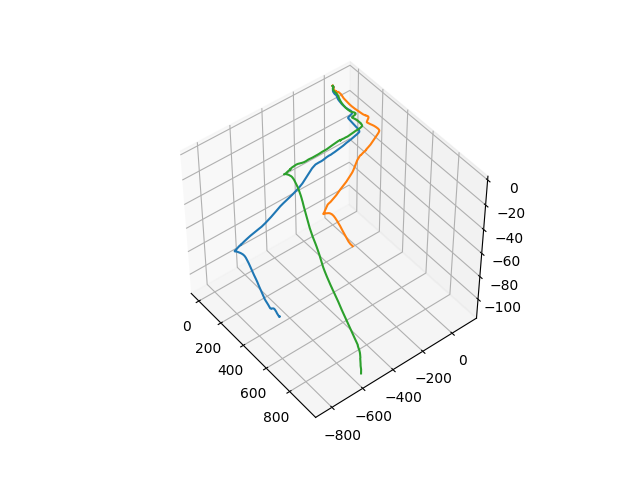
\includegraphics[width = 0.5\hsize]{figures/blackfriars_okvis_plot.png}
	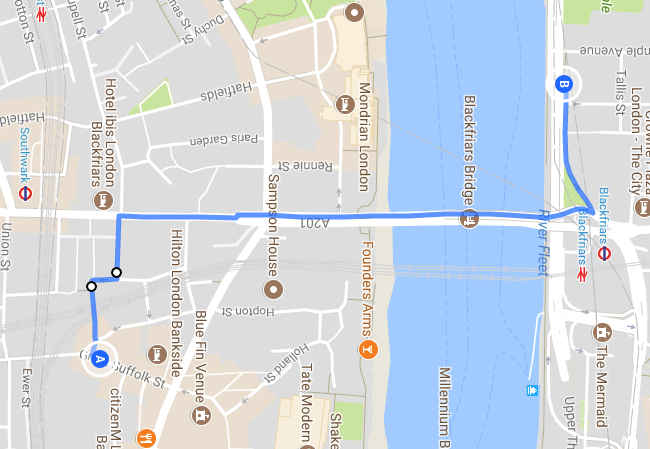
\includegraphics[width = 0.5\hsize]{figures/blackfriars_map.png}
	\caption{Okvis Paths: Left, Google Map: Right.}
	\label{blackfriars_maps}
\end{figure}

Although the Okvis paths look vastly different, the model is only interested in short segments and hence the variation is less than perceived in Figure \ref{blackfriars_maps}. The main problem with models is the ability to generalise, hence training on a limited, unbalanced dataset is tricky. So for the prediction it is assumed that someone is able to record their daily commute and train the model on that route. So the validation and test sets consist of a same route on a different day with the obvious varied lighting, traffic conditions, and traffic lights that come with the average daily commute variation.

\subsection{Objects Prediction} \label{object_model}
The objects are modelled by the Kalman filter from frame to frame and this provides a good estimate of both the direction and predicted position. Hence in a future position, say in 10 frames would simply be obtained from multiplying by a modified state-transition model.

\begin{equation}
F_{k+\mathit{n \textunderscore seconds}} = 
\begin{bmatrix}
I_{5} & \mathit{n \textunderscore seconds} \times I_{5} \\[0.3em]

0_{5 \times 5} & I_{5} \\[0.3em]
\end{bmatrix}
\end{equation}

where $\mathit{n \textunderscore seconds}$ is the number of seconds in the future to predict the position at.

\begin{equation}
\begin{aligned}
\hat{X}_{k+\mathit{n \textunderscore seconds}}(-) =  F_{k+\mathit{n \textunderscore seconds}} \hat{X}_{k-1}(+)
\end{aligned}
\end{equation}

The uncertainty of that position also increases with time, and can be taken directly from the error covariance prediction matrix. This however is updated iteratively and so it is easy enough just to repeat Equation \ref{update_cov_kalman} $ \big (\frac{\mathit{n \textunderscore seconds}}{\Delta t} \big )$ times.

\begin{equation}
\begin{aligned}
P_{k+ \Delta t}(-) = F_{k} P_{k- \Delta t}(+) F_{k}^{T} + Q_{k}
\end{aligned}
\label{update_cov_kalman}
\end{equation}

However, for speed of computation an approximation can be used:

\begin{equation}
P_{k+ \mathit{n \textunderscore seconds}}(-) \approx F_{k + \mathit{n \textunderscore seconds}} P_{k- \Delta t}(+) F_{k + \mathit{n \textunderscore seconds}}^{T} + \frac{Q_{k} \times \mathit{n \textunderscore seconds}} {\Delta t}
\end{equation}
\begin{equation}
radius = \sqrt{P_{k+ \mathit{n \textunderscore seconds}}(-)}
\label{cov_kalman_approx}
\end{equation}

This method then produces a predicted position and the uncertainty in that position which can be used to create spheres of possible object positions in future frames. These can then be checked for intersection with the bike model predictions. 



\subsection{Bike Model} \label{bike_model}

The bike is deemed to be the most important model and can therefore predictions should take into account higher order features, for example the current state of the bicycle in the frame and perhaps external factors such as the surrounding environment. The problem is therefore split into two branches, one for sequence prediction of Okvis pose outputs and the other of predictions using image inputs.



\paragraph{Okvis Sequence Inputs:}
Since the model is required to learn a sequence a recurrent neural network is the obvious choice. This mimicks memory from one-frame to the next, providing $n$ previous frames to predict the $(n+1)th$ frame. The proposed architecture for this model, by no means fine-tuned but merely to provide a proof-of-concept is as follows:

\paragraph{Pose RNN Model:} \label{pose_model}
The main problem is to generalise the model to any world point. For example, the bike could be at any location or offset from the world origin and thus a huge amount of data would be needed for learning if the world location was an input. Instead, the model simply learns the difference in camera frame between frames. Note however, things such as orientation can make a large difference, if the bike is at a big angle in the world frame it will be turning quickly. This information cannot be transferred from the difference between an original frame and the next in camera frame. Hence the tilt part of the transformation matrix is added to the camera frame position and orientation of the $n$th frame in the sequence from the perspective of the $0th$ frame in the sequence Equation \ref{pose_sequence}.


\begin{equation}
X_{frame_{n}} = 
\bigg [ [I_{1 \times 3} \quad 0]T^{-1}_{WC_{0}}T_{WC_{n}} \quad , \quad C_{ez}\bigg ]
\end{equation}
\begin{equation}
C_{ez} = (T_{WS} T_{SC})^{-1}
\begin{bmatrix}
0 & 0 & 0 & 1 & 0
\end{bmatrix}^{T}
\end{equation}
\begin{equation}
y = r_{WC_{n+1}}
\label{pose_sequence}
\end{equation}

The model is formed of the layers detailed on the right of Figure \ref{network_architecture}. Given a limited input space $X = (len_{sequence}, 16)$ where the transformation matrix is flattened for use in the LSTM layers to a matrix of size $12$. The model is trained in a regression setting with labels $\mathbf{y}=[x,y,z]$ which represent the displacement from frame last of the sequence at the subsequent frame. As it would be too granular to learn from every frame, a larger time-gap between frames can be used and hence the model sequence can consist of every $k$th frame from the camera. The loss function used is mean squared error and is formulated as follows:

\begin{equation}
\begin{aligned}
mse = 
\sum_{i=0}^{n}\sum_{j=0}^{m} (\mathbf{y}_{i,j}-\hat{\mathbf{y}}_{i,j})^{2}
\end{aligned}
\label{pose_loss}
\end{equation}

where $i$ is the sequence number, $j$ is the variable prediction and therefore $m=3$ for $[x,y,z]$. The model simple as the number of features is small so learning from the pose inputs will not require a complex model. The structure is formulated below:

\noindent \begin{table}[h!]
	\centering
	\begin{tabular}{|p{3.5cm}|p{3.5cm}|p{3.5cm}|}
		\hline
		\textbf{Layer Number}&\textbf{Layer} & \textbf{Size}                                  \\ \hline
		1  & LSTM   &   32     \\ \hline
		2  & LSTM   &   32     \\ \hline
		3  & LSTM   &   32    \\ \hline
		4  & Dense  &   3    \\ \hline		
	\end{tabular}
	\caption{Pose Model Dimensions}
\end{table}

%TODO update graphic
\noindent \begin{figure}[h!]
	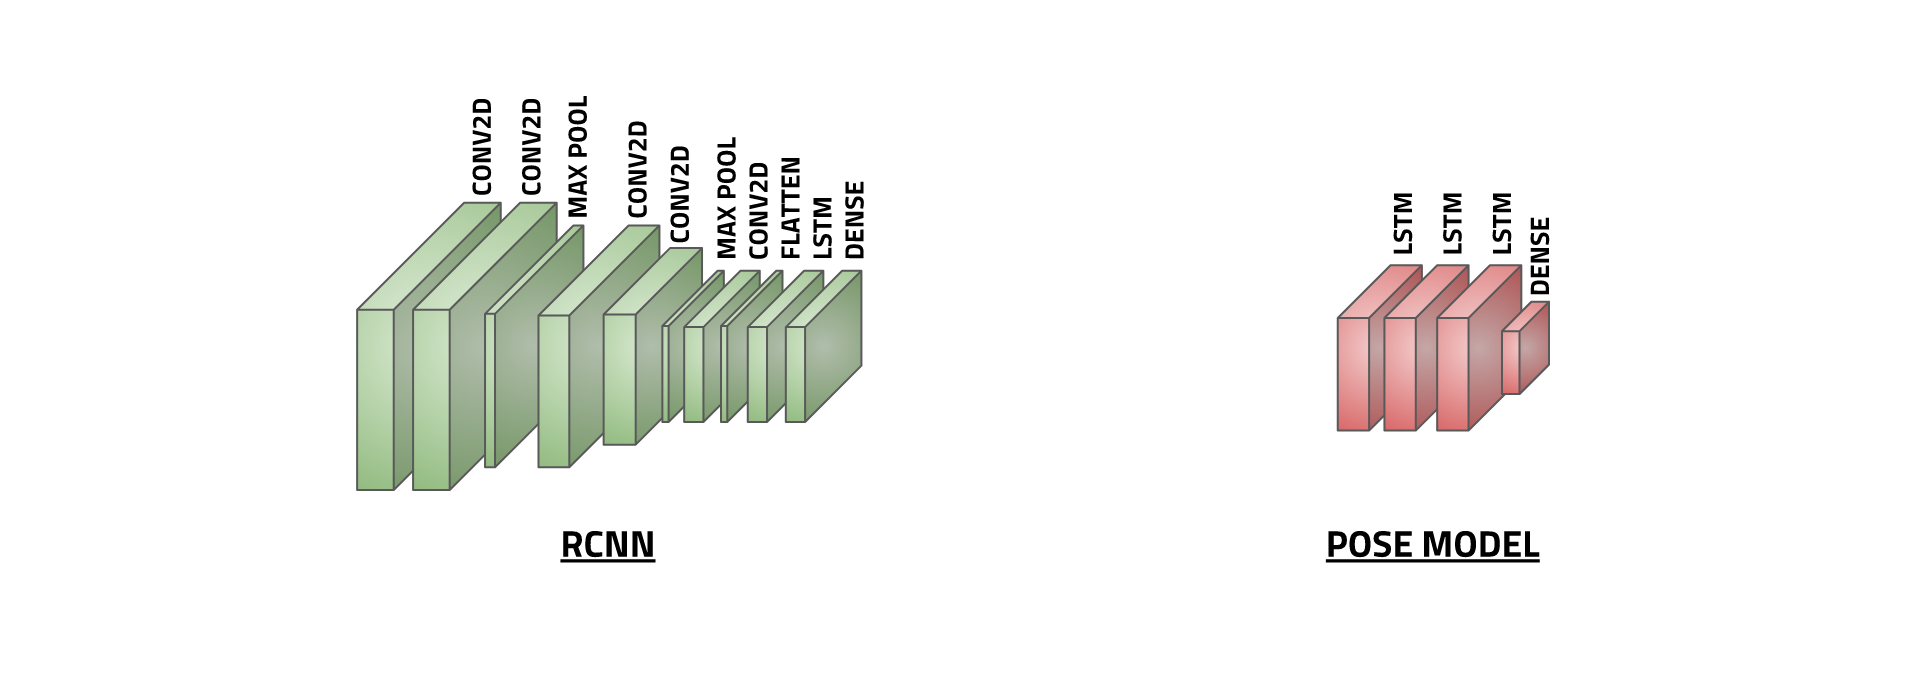
\includegraphics[width = 1.0\hsize]{figures/Networks.png}
	\caption{RCNN Architecture: Left, Pose Architecture: Right.}
	\label{network_architecture}
\end{figure}

\paragraph{Images RCNN Model:} \label{images_rcnn}
For the image section of the model, a standard convolutional learning approach is adopted as described in Section \ref{Cnn_section}. The loss function for the RCNN model is the same as Equation \ref{pose_loss}, as once again this is a regression problem. The images are fed into the network and the difference predicted much like before. The only variation is the data input and the flattening layer before the LSTM. A convolutional layer outputs a number of 3D tensors $(w,h,d)$ which is not compatible with the LSTM or dense matrices. Hence a flattening layer converts the tensors into a shape $(sequence \textunderscore length, w \times h \times d)$ for input into the final network layers. Additionally some extra pre-processing is required, since images are scaled from 0 to 255 it is hard to learn. Hence the images are simply scaled to between $(-1,1)$ by $(image-127.5)/127.5$.

\noindent \begin{table}[h!]
	\centering
	\begin{tabular}{|p{3.5cm}|p{3.5cm}|p{3.5cm}|}
		\hline
		\textbf{Layer Number}&\textbf{Layer} & \textbf{Size}                                  \\ \hline
		1  & Convolutional   &   32     \\ \hline
		2  & Convolutional   &   32     \\ \hline
		3  & Max Pooling     &   N/A    \\ \hline
		4  & Dropout (.25)   &   N/A    \\ \hline
		5  & Convolutional   &   16     \\ \hline
		6  & Convolutional   &   16     \\ \hline
		7  & Max Pooling     &   N/A    \\ \hline  
		8  & Dropout (.25)   &   N/A    \\ \hline
		9  & Flatten         &   N/A    \\ \hline
		10 & LSTM            &   64     \\ \hline   
		11 & Dense           &   32     \\ \hline 
		12 & Dense           &   3      \\ \hline 
		                                                                           
	\end{tabular}
\caption{RCNN Dimensions}
\end{table}


\paragraph{Optimising Learning Rate and Decay:}
Adam optimiser, a common solver for deep learning problems requires a number of parameters which are all set as the default recommended from the paper \cite{DBLP:journals/corr/KingmaB14} $\beta_{1}=0.9$,$\beta_{2}=0.999$,$\epsilon=10^{-8}$ these are adaptive moment parameters that control the algorithm's descent into minima. However learning rate and learning rate decay are problem specific and can vastly impair the ability of a model to learn correctly. Hence a logical approach to selection of the right values is required. A grid search method was chosen and loss characteristics at epoch 200 compared to get a reasonable approximate for the correct learning rate.


\noindent \begin{figure}[h!]
	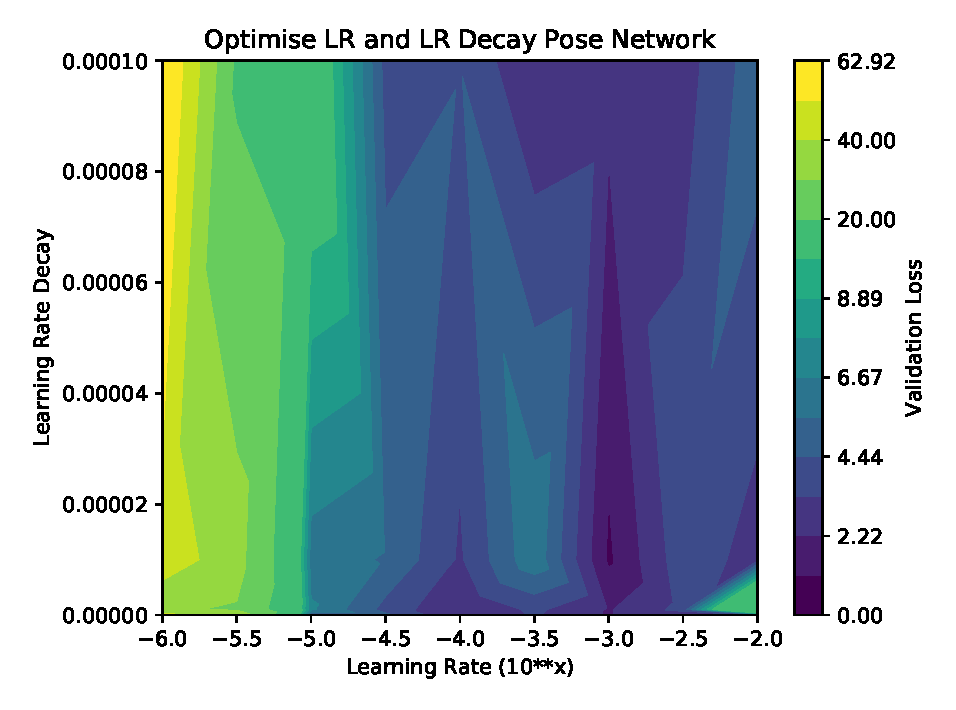
\includegraphics[width = 0.5\hsize]{figures/pose_lr_lr_decay_graph_.eps}
	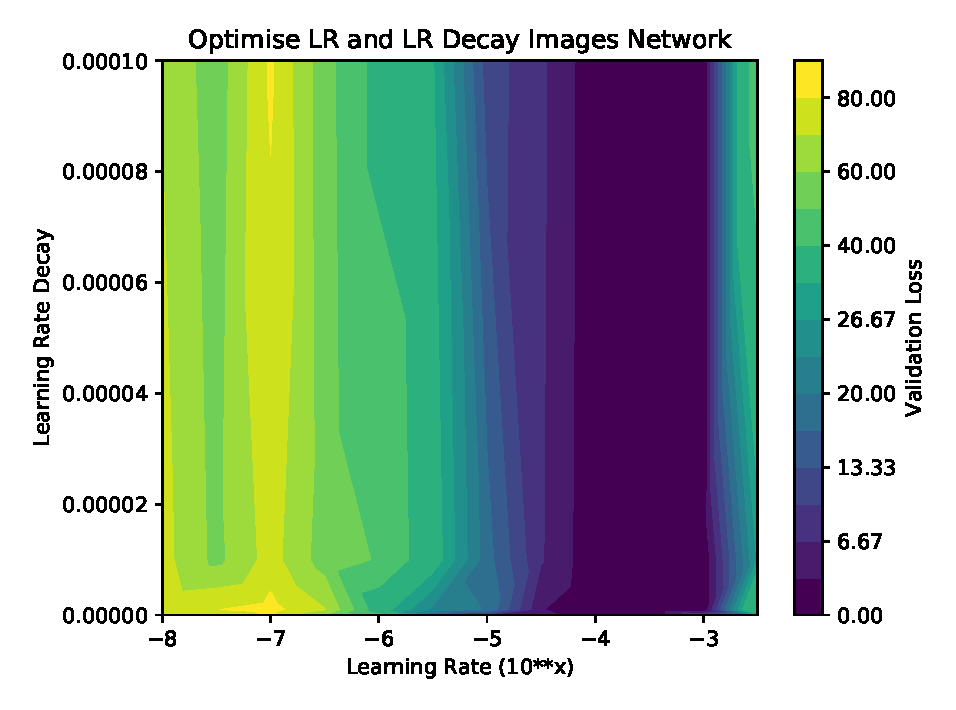
\includegraphics[width = 0.5\hsize]{figures/images_lr_lr_decay_graph_.eps}
	\caption{Pose Lr and Lr Decay Grid: Left, Images Network Optimisation: Right.}
	\label{lr_and_decay_grid}
\end{figure}

Both the image and pose model appear to prefer higher learning rates around the $10^{-4},10^{-3}$ region. Learning rate decay has little influence to the results of the images network which has an optimal values of:

\noindent \begin{table}[h!]
	\centering
	\begin{tabular}{|p{1.0cm}|p{3.0cm}|p{3.0cm}|p{3.0cm}|}
		\hline
		\textbf{Rank}&\textbf{Learning Rate} & \textbf{Decay} &  \textbf{Validation Loss}       \\ \hline
		1  & $10^{-3.5}$   &   0 & 0.11     \\ \hline
		2  & $10^{-3}$   &   $10^{-6}$ & 0.14     \\ \hline
		3  & $10^{-3.5}$    &    $10^{-5}$ & 0.19   \\ \hline
		
	\end{tabular}
	\caption{Image Learning Rate vs Learning Rate Decay}
	\label{image_lr_lr_decay_table}
\end{table}

From experience, and logically it is preferable to take an optimal value with decay for longer runs of the network. As the optimisation is performed over only 200 epochs often the lower learning rates with decay perform better in the long-run. Hence the parameter choice ranked no.2 in Table \ref{image_lr_lr_decay_table} is used for the final model. A part to note is that the loss function is mean squared error and so $0.11$ loss is roughly equivalent to $0.3m$. The pose model interestingly has a higher optimal loss than the images model, but this is likely due to the number of epochs and model complexity in using the same route for the test set (different days but same route). The pose model is simple and therefore can train much faster than the images model so it should be trained for longer for a fair comparison. The images model has more layers and thus may overfit the route whilst the pose model may perform better on unknown routes.

\noindent \begin{table}[h!]
	\centering
	\begin{tabular}{|p{1.0cm}|p{3.0cm}|p{3.0cm}|p{3.0cm}|}
		\hline
		\textbf{Rank}&\textbf{Learning Rate} & \textbf{Decay} &  \textbf{Validation Loss}       \\ \hline
		1  & $10^{-3}$   &  $10^{-5}$ & 0.91     \\ \hline
		2  & $10^{-3}$   &   $10^{-6}$ & 2.11    \\ \hline
		3  & $10^{-4}$    &    $10^{-6}$ & 2.20   \\ \hline
		
	\end{tabular}
	\caption{Pose Learning Rate vs Learning Rate Decay}
	\label{pose_lr_lr_decay_table}
\end{table}
 
The highest ranked parameters in Table \ref{pose_lr_lr_decay_table} are taken forwards to the next stage of the process, optimising the layer dimensions.
 
\subsubsection{Bayesian Optimisation Layer Dimensions:}
The images and pose model are first optimised with respect to learning rate and learning rate decay with a grid search. From there each is optimised with respect to layer dimensions via Bayesian Optimisation. It is questionable as to the order that this should occur in but it is inevitable cyclic so for simplicity learning rate and decay are optimised once as is layer size.



\noindent \begin{figure}[h!]
	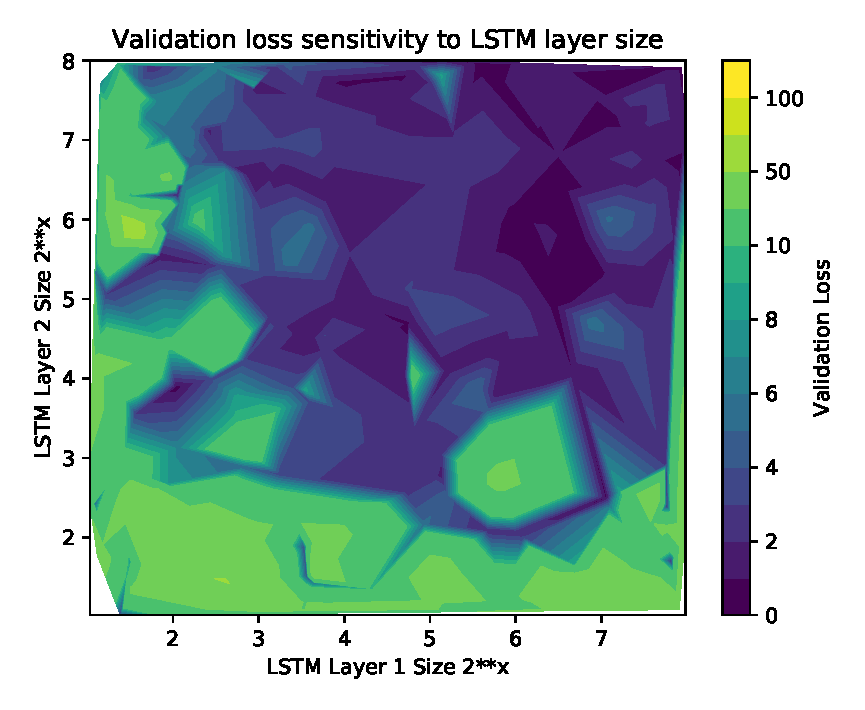
\includegraphics[width = 0.5\hsize]{figures/pose_lstm1_lstm2_graph_.eps}
	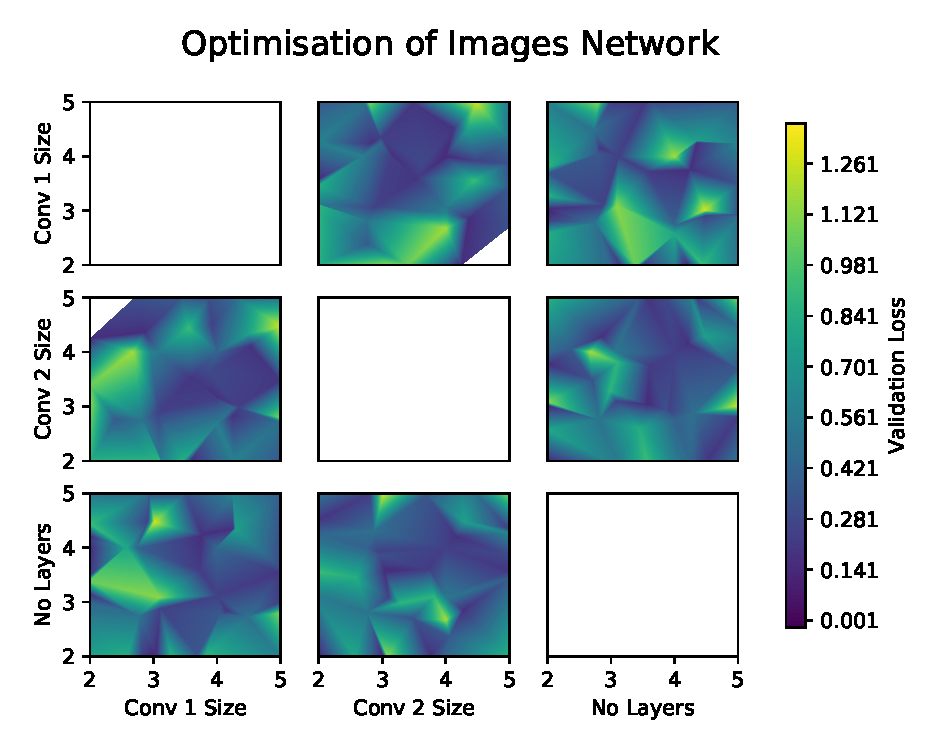
\includegraphics[width = 0.5\hsize]{figures/opt_bayes_images_nn.eps}
	\caption{Pose Layer Optimisation: Left, Images Network Optimisation: Right.}
	\label{bayes_opt_fig}
\end{figure}

\paragraph{Pose Model:} As the pose model was once again optimised with a small number of epochs it has slightly higher loss than the images model. The results from optimising the LSTM layers are as follows:

\noindent \begin{table}[h!]
	\centering
	\begin{tabular}{|p{1.0cm}|p{3.0cm}|p{3.0cm}|p{3.0cm}|}
		\hline
		\textbf{Rank}&\textbf{LSTM 1 Size} & \textbf{LSTM 2 Size} &  \textbf{Validation Loss}       \\ \hline
		1  & $2^{6.44} = 87$   &  $2^{6.25}=77$ & 0.42     \\ \hline
		2  & $2^{6.04}=63$   &  $2^{5.7}=53$ & 0.43   \\ \hline
		3  & $2^{2.03}=4$    & $2^{3.9}=15$ & 0.48   \\ \hline
		
	\end{tabular}
	\caption{Pose Layer Size Bayesian Optimisation}
	\label{pose_bayes_table}
\end{table}

The second best and best result are narrowly different, so the second best, and simpler model from Table \ref{pose_bayes_table} was then taken forward as the final dimensions for the network, and is used in the complete model.

\paragraph{Images Model:}
The images model is optimised in 3 dimensions, two involve the size of CNN layers and one is the number of layers in the network. The network has blocks of convolutional layers (Figure \ref{network_architecture}), optimising the number of layers determines whether there are one or two convolutional layers in each block. Simultaneously, the size of the layers in those blocks is also optimised.


\noindent \begin{table}[h!]
	\centering
	\begin{tabular}{|p{1.0cm}|p{2.3cm}|p{2.3cm}|p{1.5cm}|p{1.5cm}|p{2.2cm}|}
		\hline
		\textbf{Rank}&\textbf{Block 1 Size} & \textbf{Block 2 Size} &  \textbf{Block 1 Layers}   &  \textbf{Block 2 Layers} &  \textbf{Validation Loss}     \\ \hline
		1  & $2^{4.34} = 20$   &  $2^{5.0}=32$ & 1 & 1 & 0.1     \\ \hline
		2  & $2^{3.57}=12$   &  $2^{5.0}=32$ & 2 & 2 & 0.11   \\ \hline
		3  & $2^{5.0}=32$    & $2^{5.0}=32$ & 2 & 1 &  0.13   \\ \hline
		
	\end{tabular}
	\caption{Images Model Bayesian Optimisation}
	\label{images_bayes_table}
\end{table}


Interestingly the images model prefers a simpler setup with only one convolutional layer per block. This may be due to overfitting, but since extra layers are added when combined into the total model it is beneficial to keep the simpler architecture as it is likely to perform better. Hence the final model architecture is presented in Figure \ref{final_models}


\subsubsection{Final Optimised Models}

\noindent \begin{figure}[h!]
	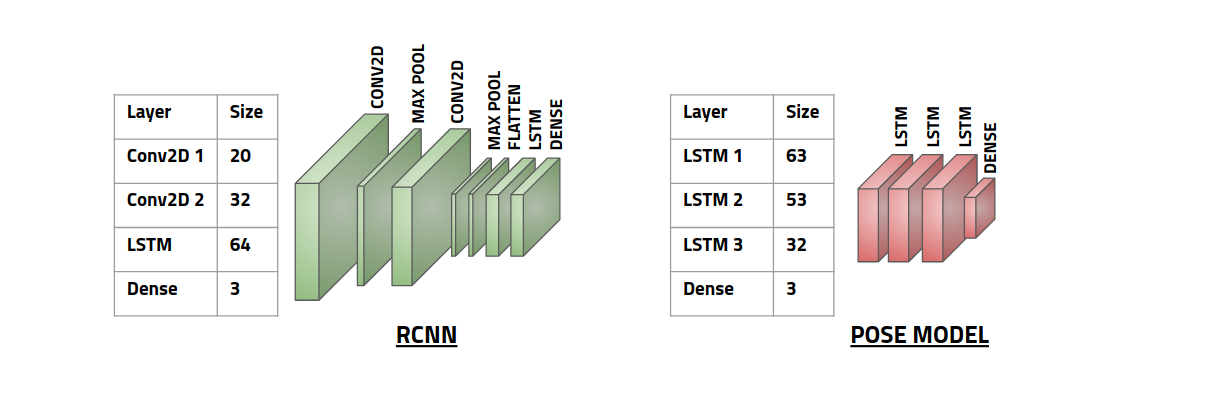
\includegraphics[width = 1.0\hsize]{figures/final_models.png}
	\caption{Final Images Model: Left, Pose Model: Right.}
	\label{final_models}
\end{figure}


\subsubsection{Total Model:}
Both models discussed in this section can be trained separately to obtain predictions of the future pose. A naive estimation would take weighted predictions and sum for a final prediction result. The final layers of these networks however could infer details from each-other to inform the pose estimation. This can only be done in a branched network that uses both inputs effectively and concatenates the outputs for some final layers. The proposed model is graphed in Figure \ref{total_network_architecture}, it has two inputs tensors of the images plus pose data and three output variables which is the predicted $[x,y,z]$.

\noindent \begin{figure}[h!]
	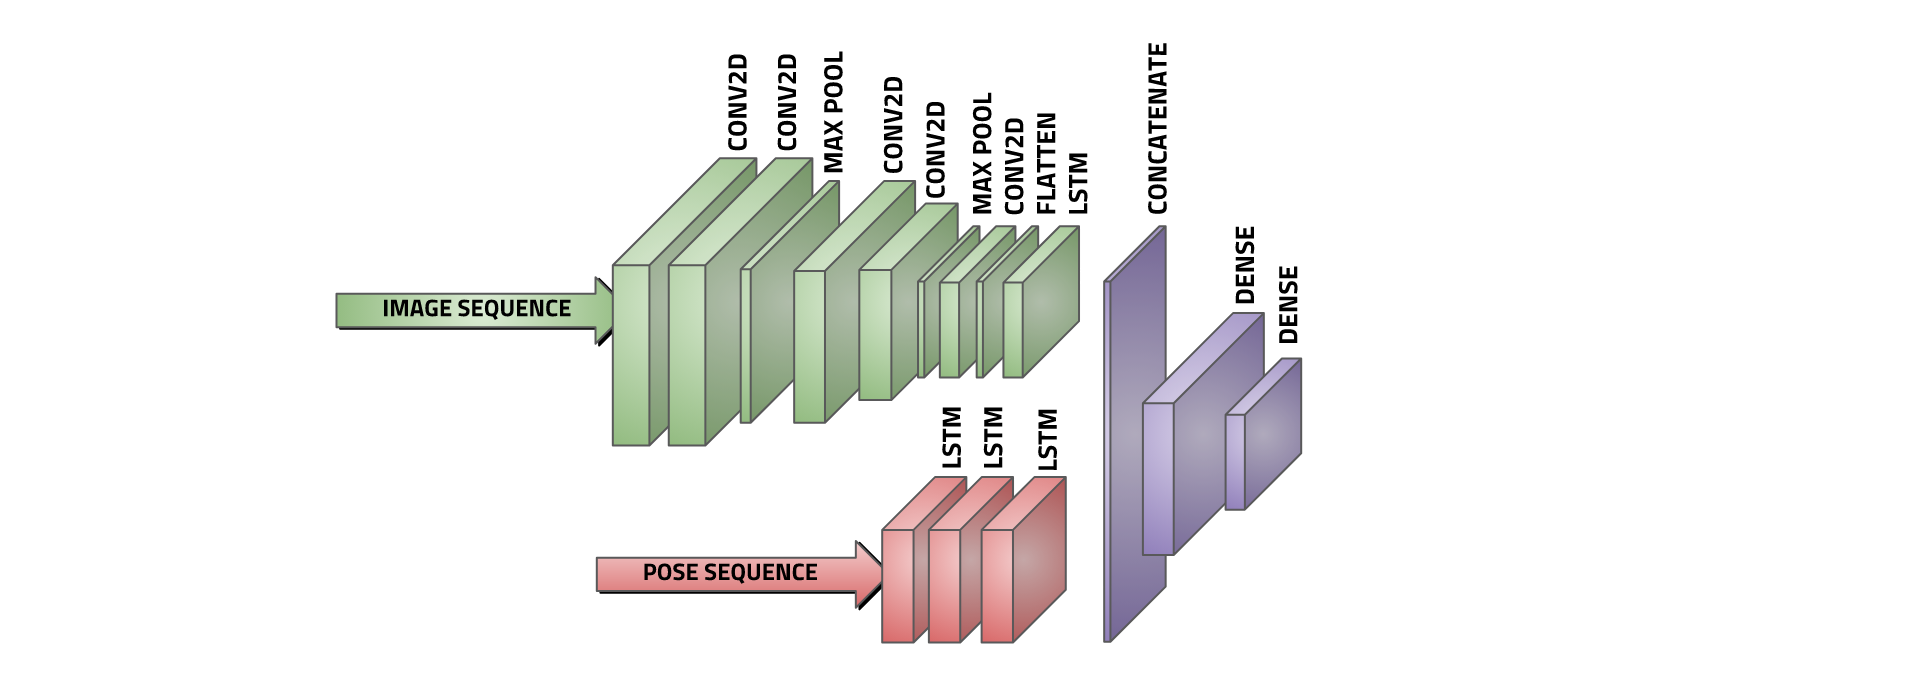
\includegraphics[width = 1.0\hsize]{figures/final_model.png}
	\caption{Complete Network Architecture.}
	\label{total_network_architecture}
\end{figure}

\paragraph{Training Regime:}The network is large and so a careful training regime is required to ensure convergence to a reasonable minimum. The two initial models, the pose and RCNN images are first pre-trained to predict poses. These are the complete models described in Figure \ref{network_architecture}. Once this training process is complete the weights are used in the larger branched model. These layers are then frozen and the final dense layers are trained. Finally all layers are unfrozen and the whole model is trained with a lower learning rate to fine-tune the weights.


For the final training, the frame gap was increased to $1s$ and hence there is a higher loss from the data. It is not excessive however with  a final loss of $1.8$ which equates to $1.3m$ uncertainty which is acceptable for future use. This uncertainty can be used in the next section to determine the possible locations of the bike in the future and detect if a collision is likely.


\noindent \begin{figure}[h!]
	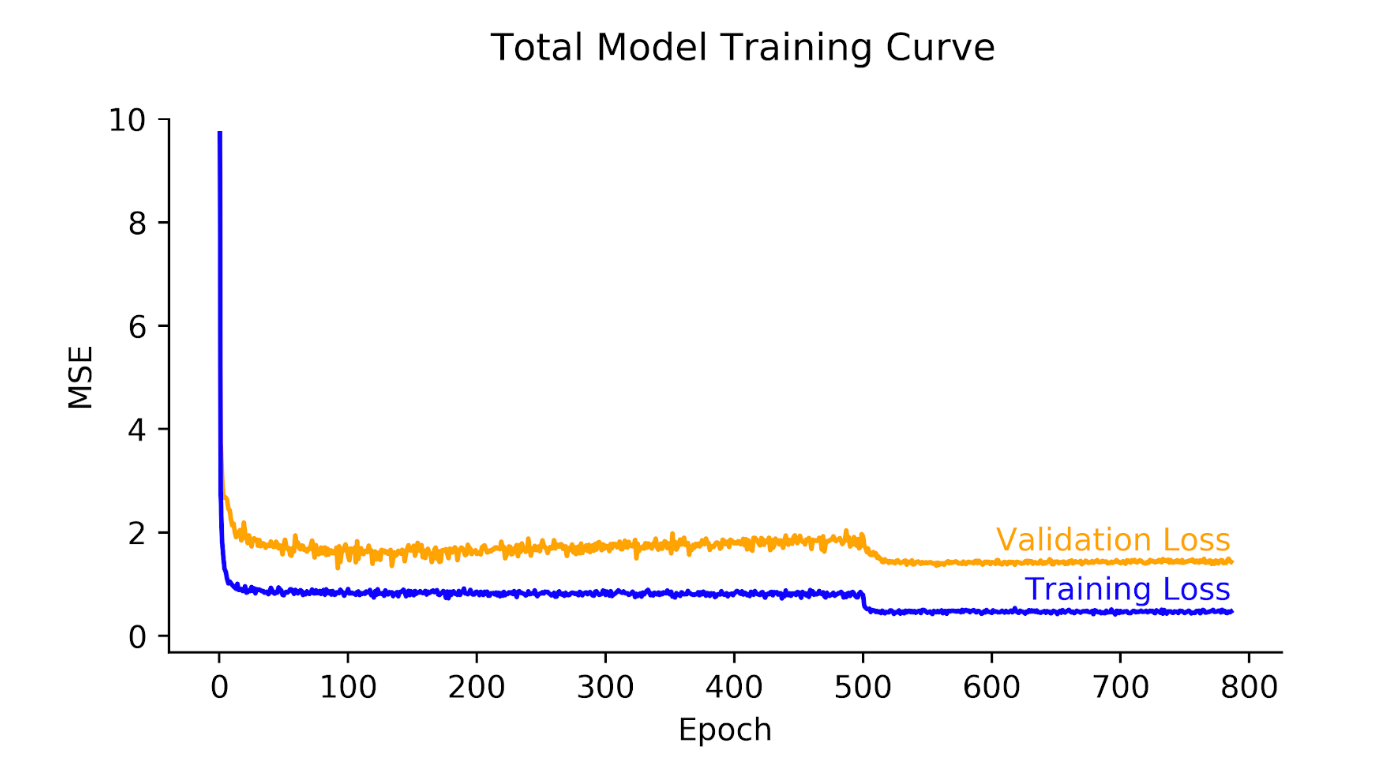
\includegraphics[width = 1.0\hsize]{figures/total_model_training.png}
	\caption{Complete Network Training.}
	\label{total_training_curve}
\end{figure}

\paragraph{Summary}
In this section a new model for cyclist movement prediction has been explored, the combination of images and pose data. This is expected to perform well with larger times between predictions. However, at smaller time gaps the model is too complex and overfits the data which means that a linear model often performs better on the validation set. It is therefore a balance between model complexity and the required time-frame of prediction. In this case a timeframe of c.1-2s is reasonable as the Mask-RCNN model cannot detect small objects that are further away with adequate accuracy and a bike can move at around 10m/s. This section has proven the ability of the model to predict accurately. Since models such as this are complex and require significant computational power it may be beneficial to join the image-segmentation network and prediction network. This would allow them to share some of the convolutional layers and reduce computational overhead but requires extensive modifications to Mask-RCNN. The outcome of this section is a reliable model that can be used in the next section for collision detection between moving objects and the cyclist. 

\subsection{Collision Detection Module}
The collision detection module takes the predicted paths from both the cyclist and object models (Sections \ref{bike_model},\ref{object_model}), and their respective uncertainties. It can then check the distance between the predicted points:

\begin{equation}
\begin{aligned}
dist = \sqrt{( (x_{c}-x_{o})^{2} + (y_{c}-y_{o})^{2}}
\end{aligned}
\label{distance_eq}
\end{equation}

where $x_{c}$ is the predicted cyclist location and $x_{o}$ is the predicted object location at time $t$. This can then be used with the uncertainty circle to see if the points could overlap.

\begin{equation}
\begin{aligned}
\begin{cases}
dist < R_{bike} + R_{obj} \quad \textbf{Check IOU} \\
dist > R_{bike} + R_{obj} \quad \textbf{Continue}
\end{cases} \\
R_{k} = \sqrt{var_{k}}
\end{aligned}
\label{horn_eq}
\end{equation}


One problem is that when the Kalman filter is highly uncertain it may predict a potential collision when there is little likelihood of it occurring so a solution can be to look at the intersection over union of the two circles.

\noindent \begin{figure}[h!]
	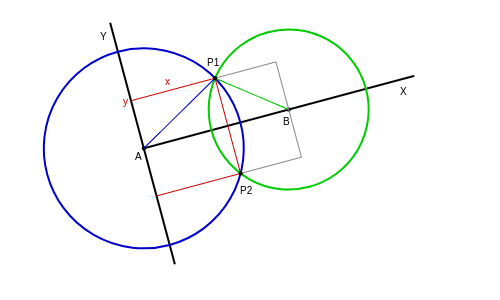
\includegraphics[width = 0.5\hsize]{figures/points_intersecting_circles.png}
	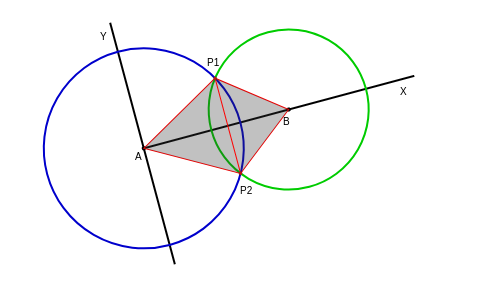
\includegraphics[width = 0.5 \hsize]{figures/two_intersecting_circles.png}
	\caption{Intersecting Points on Circle \cite{circle_intersection_point}, Right: Area of Two Intersecting Circles \cite{circle_intersection}}
	\label{two_intersect_points}
	\label{two_intersect_circles}
\end{figure}

\paragraph{Points of intersection}
The first step to calculate where the circles overlap. This is detailed in figure \ref{two_intersect_points}, point can form a triangle in each circle between the y axis, x axis and a line of length $R_{o},R_{c}$ passing through the circle's origin.


\begin{equation}
\begin{aligned}
x^{2} + y^{2} = A_{r}^{2} \\
(d^{2}-x^{2}) + y^{2} = B_{r}^{2}
\end{aligned}
\label{inter_point_eq1}
\end{equation}


Solving for $x$ and $y$ yields:

\begin{equation}
\begin{aligned}
x = \frac{A_{r}^{2} - B_{r}^{2} + d^{2}}{2d} \\
y_{1,2} = \pm \sqrt{A_{r}^{2} - x^{2}}
\end{aligned}
\label{inter_point_eq2}
\end{equation}

Transforming the values into unit vectors and solving for the final point locations gives:

\begin{equation}
 \overrightarrow{e_{1}} = \frac{ \overrightarrow{B}- \overrightarrow{A}}{|  \overrightarrow{B} -  \overrightarrow{A} |} 
= 
\frac{1}{d}
\begin{bmatrix}
B_{x} - A_{x} \\
B_{y} - A_{y}
\end{bmatrix} 
\end{equation}
\begin{equation}
\overrightarrow{e_{2}} =
rot(90) \overrightarrow{e_{1}} =
\begin{bmatrix}
0 & -1 \\
1 & 0
\end{bmatrix}
\overrightarrow{e_{1}}
\end{equation}
\begin{equation}
\overrightarrow{P_{1,2}} = \overrightarrow{A}+x \cdot \overrightarrow{e_{1}} \pm y \cdot \overrightarrow{e_{2}}
\label{inter_point_eq3}
\end{equation}

The final check is to determine if one circle is within the other and hence there are no intersection points. This is given by checking that the distance is greater than the absolute difference between radii, i.e.


\begin{equation}
\begin{aligned}
dist < |B_{r} - A_{r}| = \textbf{Circle Inception}
\end{aligned}
\label{circle_inception}
\end{equation}


\paragraph{Area of Intersection}

Given the equations for $x$ and $y$ shown in the last section. The angles $\theta_{A}$ and $\theta_{B}$ can be calculated. The idea for calculation is simple, the intersection area is the area of the segment minus the area of the triangle.


\begin{equation}
\begin{aligned}
\theta_{A} = 2sin^{-1} \bigg ( \frac{y}{A_{r}} \bigg )
\\
\theta_{B} = 2sin^{-1} \bigg ( \frac{y}{B_{r}} \bigg )
\end{aligned}
\label{circle_area_eq1}
\end{equation}

From this the area of the two triangles are:

\begin{equation}
\begin{aligned}
area_{t,1} = y \sqrt{A_{r}^{2} - y^{2}} \\
area_{t,2} = y \sqrt{B_{r}^{2} - y^{2}}
\end{aligned}
\label{circle_area_eq1}
\end{equation}


Finally the area of the intersection is calculated using:

\begin{equation}
\begin{aligned}
area = A_{r}^{2}sin^{-1} \big ( \frac{y}{A_{r}}) + B_{r}^{2}sin^{-1} \big ( \frac{y}{B_{r}}) + y \bigg ( \sqrt{A_{r}^{2} - y^{2}} + \sqrt{B_{r}^{2} - y^{2}} \bigg )
\end{aligned}
\label{circle_area_eq1}
\end{equation}

\paragraph{Intersection Over Union}
In order to better understand the likelihood the circle approximate is used. This, although not exact as Gaussians are a bell shape is a fast and closed form approximate for the probability of collision. The IOU of the circles is the best measure, a higher IOU clearly means a more probably crash. It can be calculated from previous results:


\begin{equation}
\begin{aligned}
IOU = \frac{area_{intersection}}{ area_{c1} + area_{c2} - area_{intersection}}
\end{aligned}
\label{circle_area_eq1}
\end{equation}

\paragraph{Moving Objects}
It is important to check that the object itself is moving. If the cyclist is heading towards a parked car it is less likely that the cyclist has not seen it or that the object will cross their path. So the final check is a simple threshold of the Kalman filter prediction. As part of the state, the velocity of the object is predicted which informs the collision detection module if the object in question is moving or not.


%%%%%%%%%%%%%%%%%%%%%%%%%%%%%%%%%%%%
\chapter{Experimental Results}

\section{System Evaluation}

\subsection{Mask-RCNN}
In applying Mask-RCNN to the specific urban environment there have been a number of interesting outcomes. On the whole, the system is robust, often detecting images well and so there are rarely gaps when an object is detected in one frame and not the next. A number of incorrect classifications often provide a worry, for example, the classification of road paint can cause a problem to the system (Figure \ref{mrcnn_fail}). This often happens with road markings of bicycles that are relatively convincing examples, this is perhaps solvable with using these examples as part of the null class during training and could be investigated in future work.

\noindent \begin{figure}[h!]
	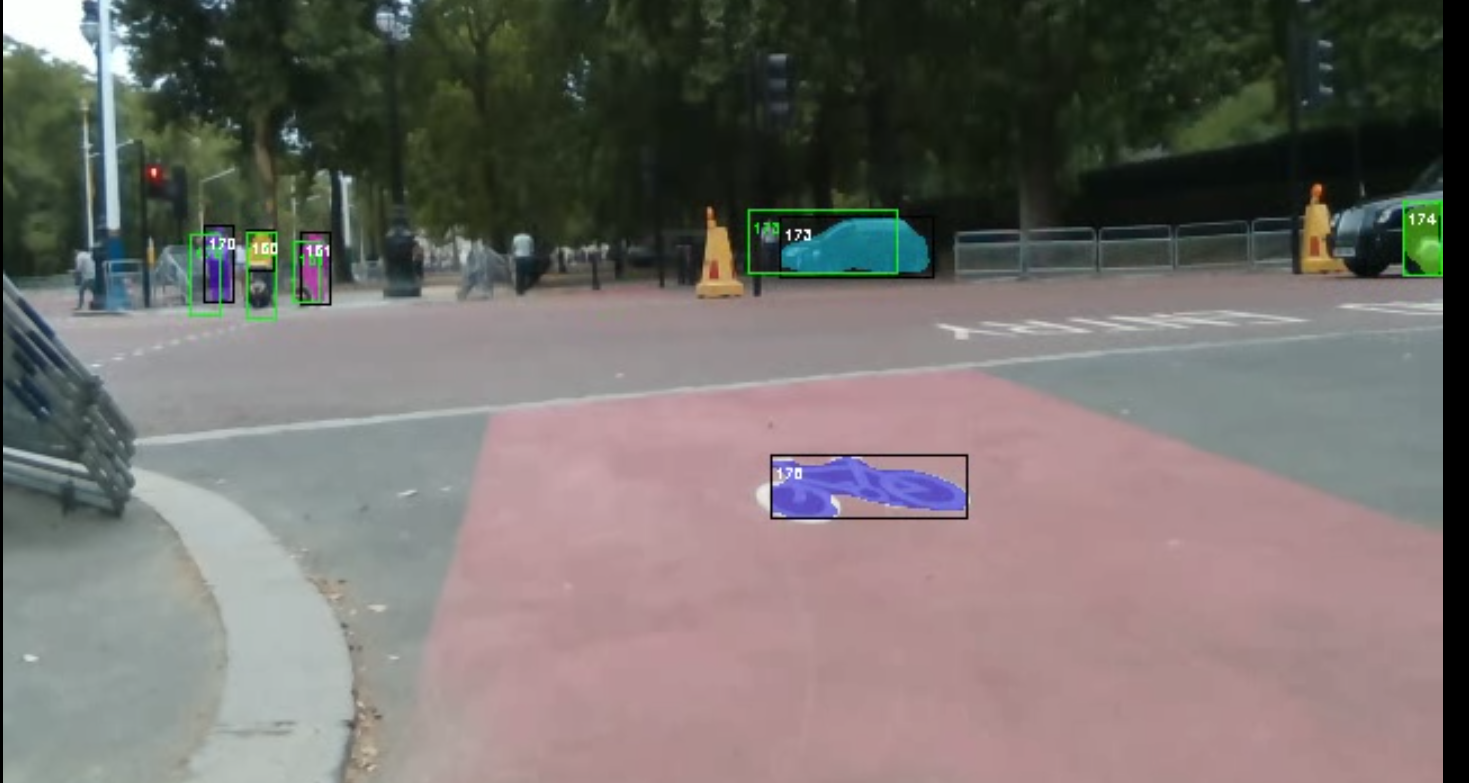
\includegraphics[width = 1.0\hsize]{figures/segment_bike.png}
	\caption{Mask-RCNN failure}
	\label{mrcnn_fail}
\end{figure}



\subsection{Cyclist Model}

The cyclist model is effective as proven in Section \ref{bike_model}, however it currently requires a new model, with respective inputs and convolutional layers. This is both slow and memory intensive, the best solution would be to integrate the model into Mask-RCNN and share some of the convolutional layers. It is a significant modification however as Mask-RCNN does not use sequences of data so a novel architecture would need to be investigated.
\newline \newline
The other, far simpler solution is to make use of the Kalman filter mentioned in Section \ref{kalman_matching}, this is less complex and also faster than a neural network model. It does however have drawbacks in accuracy that the network does not, so implementation would be on a hardware specific basis. The faster the hardware, the more viable a complex model is.

\subsection{Depth Camera}

The intel realsense depth camera is typically used in indoor environments as it operates with a small laser. This, as is expected works less well in highly lit environments. The extent of the problem, however is often drastic and can cause okvis to perform poor estimations of pose and hence is unable to determine the bicycle location. This problem could be eliminated completely by using a stereo camera system or by relying on GPs in bright lighting conditions.

\subsection{Crash Sequence Evaluation}

In order to determine the effectiveness of the system, it is important to know that the system will not produce numerous false positives and be an irritation to users, but also correctly activate when required. Therefore there are two sequences of images collected, one with a staged incident where the values have been tweaked to be more sensitive, and hence reduce the danger in conducting the experiment. The other sequence contains a parked car, which is detected but also determined to no be moving and hence of no danger to the rider.

\noindent \begin{figure}[h!]
	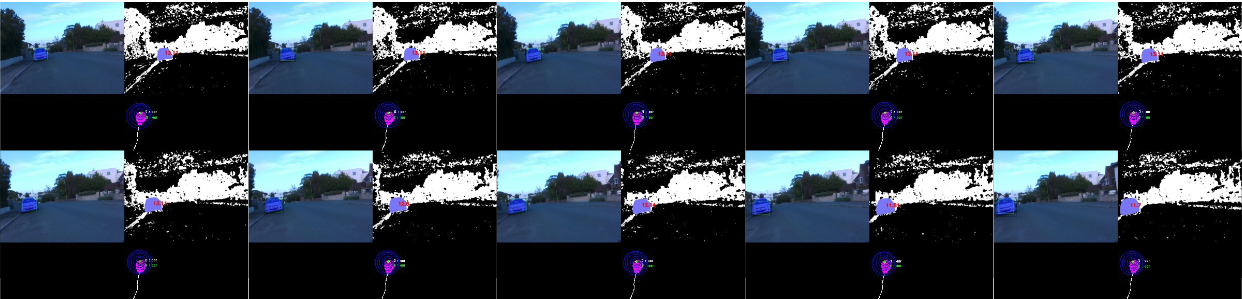
\includegraphics[width = 1.0\hsize]{figures/no_crash.png}
	\caption{Parked Car Evaluation}
	\label{mrcnn_fail}
\end{figure}

It is hard to get a sequence into the report but comparison to the staged crash shows that it is evident the car is detected but not deemed a threat to the cyclist. This is even though at some stage the cyclist is travelling directly towards the vehicle.

\noindent \begin{figure}[h!]
	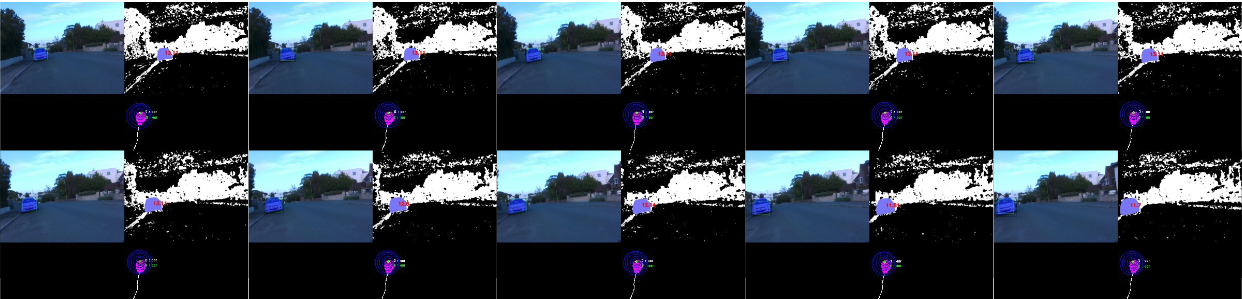
\includegraphics[width = 1.0\hsize]{figures/no_crash.png}
	\caption{Staged Crash}
	\label{mrcnn_fail}
\end{figure}



\chapter{Conclusion}

\subsection{Contributions}

In section \ref{Depth_approx}, it was stated how poor hardware accuracy with regards to depth estimates can be modified with prior knowledge of object sizes in segmented images. This both reduces depth outliers and provides the Kalman filter with less noisy data to track.

Section \ref{kcf_kernels} discusses how to modify the KCF tracker (Section \ref{kcf_background}) for use in the multi-class case. This is then later used in combination with Brisk, class, and Kalman matching for object identification between each frame Section \ref{matching_combining_methods}.

The final contributions of this report involve the tracking and prediction models for both objects (Section \ref{object_model}) and cyclists (Section \ref{bike_model}). The object model used a modification to a Kalman filter to get the predictions and uncertainties whilst a novel recurrent neural network architecture was developed for bike model prediction. The network in question learns from both image and pose data to predict the future bicycle state. From here the object collision module can use the states and uncertainties to calculate the intersection over union of the future states and determine if a collision is likely.

\subsection{Future Work}

\paragraph{Speed} It is clear that this product is much needed in the arsenal of a cycling commuter but in its current state it is not able to be implemented. The sub-real-time results are too slow for effective use. Therefore, with simpler updated hardware and software it may become less accurate but would be useful in the cycling environment until newer technology is available that can increase accuracy to the current level. Also a pure implementation in a faster language such as cpp could help with this, most of the functions used e.g. (Keras, numpy, Tensorflow) implement c sub-routines, but other parts of the code could equally be sped-up by being ported to c or cpp instead of running python.

\paragraph{Object Detection} It is clear, at the time of writing, that the only real-time method of object detection that could be applicable to cycling is tiny-yolo \cite{DBLP:journals/corr/RedmonDGF15}. This is a bounding box approach that runs at c. 80fps on a laptop gpu, and can now be used on a mobile. With this, however comes the deficit of being unable to segment the image like in Mask-RCNN for depth prediction. A lightweight version therefore could use the depth approximation developed in Section \ref{Depth_approx}. Although not perfect, combined with a 3d appreciated of the environment it could be effective, and most importantly fast enough for use. 

\paragraph{SLAM} Although Okvis is effective, the poor quality depth camera images render it less reliable outside than in indoor environments. This would typically not be acceptable on a final system so perhaps incorporating GPS measurements as well as Okvis would be beneficial. Okvis is great for areas where there is no GPS available, such as tunnels, where lighting is also reduced. Okvis is capable of running from a single camera and so the removal of a depth stream would also not hinder it greatly, especially if a stereo camera system was employed instead.



\chapter{Ethics}

\subsection{Modification for Military Purposes}
The code presented in this report, although strictly for civilian applications does have the potential to be modified for military use. It obviously provides the ability to track people and objects from frame-to-frame. This however, is not in a real-time context at present and would require significant modification for use in such an environment that would be conducive to a military application. However, that being said little modification is needed for a simple tracking application from CCTV data for example. This would not need to run at real time and could be a potential source of misuse.

\subsection{Other Ethics Issues}

The code developed is intended to offer a basis for an early warning system to cyclists in urban environments. Hence a number of the inherent ethical problems with, for example the autonomous vehicle space are also applicable to this project. The potential over-reliance on such a system of cyclists could be dangerous and allow for lack of attention and potential accidents when the system is unable to detect a collision. That having been said, it is evident that there is a need for such a system for cyclists and so the benefits would clearly outweighs the disadvantages in such a case.

\section{Ethics Checklist}

% You need the following added in your includes:
% \usepackage[table]{xcolor}
% \usepackage{amssymb}

% Check off the boxes using: \checkmark


\renewcommand*{\arraystretch}{1.3}
\begin{longtable}{ |p{13.2cm}|p{0.6cm}|p{0.6cm}| }
	\hline
	& \bf Yes & \bf No \\
	\hline
	
	\multicolumn{3}{|l|}{\cellcolor{green!25}\bf Section 1: HUMAN EMBRYOS/FOETUSES} \\
	\hline
	
	Does your project involve Human Embryonic Stem Cells? & & \checkmark \\
	\hline
	
	Does your project involve the use of human embryos? & & \checkmark \\
	\hline
	
	Does your project involve the use of human foetal tissues / cells? & & \checkmark \\
	\hline
	
	\multicolumn{3}{|l|}{\cellcolor{green!25}\bf Section 2: HUMANS} \\
	\hline
	
	Does your project involve human participants? & & \checkmark \\
	\hline
	
	\multicolumn{3}{|l|}{\cellcolor{green!25}\bf Section 3: HUMAN CELLS / TISSUES} \\
	\hline
	
	Does your project involve human cells or tissues? (Other than from “Human Embryos/Foetuses” i.e. Section 1)? & & \checkmark \\
	\hline
	
	\multicolumn{3}{|l|}{\cellcolor{green!25}\bf Section 4: PROTECTION OF PERSONAL DATA} \\
	\hline
	
	Does your project involve personal data collection and/or processing? & & \checkmark \\
	\hline
	
	Does it involve the collection and/or processing of sensitive personal data (e.g. health, sexual lifestyle, ethnicity, political opinion, religious or philosophical conviction)? & & \checkmark \\
	\hline
	
	Does it involve processing of genetic information? &  & \checkmark\\
	\hline
	
	Does it involve tracking or observation of participants? It should be noted that this issue is not limited to surveillance or localization data. It also applies to Wan data such as IP address, MACs, cookies etc. & & \checkmark \\
	\hline
	
	Does your project involve further processing of previously collected personal data (secondary use)? For example Does your project involve merging existing data sets? & & \checkmark \\
	\hline
	
	\multicolumn{3}{|l|}{\cellcolor{green!25}\bf Section 5: ANIMALS} \\
	\hline
	
	Does your project involve animals? & & \checkmark \\
	\hline
	
	
	\multicolumn{3}{|l|}{\cellcolor{green!25}\bf Section 6: DEVELOPING COUNTRIES} \\
	\hline
	
	Does your project involve developing countries? & & \checkmark \\
	\hline
	
	If your project involves low and/or lower-middle income countries, are any benefit-sharing actions planned? & & \checkmark \\
	\hline
	
	Could the situation in the country put the individuals taking part in the project at risk? & & \checkmark \\
	\hline
	
	\multicolumn{3}{|l|}{\cellcolor{green!25}\bf Section 7: ENVIRONMENTAL PROTECTION AND SAFETY} \\
	\hline
	
	Does your project involve the use of elements that may cause harm to the environment, animals or plants? & & \checkmark \\
	\hline
	
	Does your project deal with endangered fauna and/or flora /protected areas? & & \checkmark \\
	\hline
	
	Does your project involve the use of elements that may cause harm to humans, including project staff? & & \checkmark \\
	\hline
	
	Does your project involve other harmful materials or equipment, e.g. high-powered laser systems? & & \checkmark \\
	\hline
	
	
	\multicolumn{3}{|l|}{\cellcolor{green!25}\bf Section 8: DUAL USE} \\
	\hline
	
	Does your project have the potential for military applications? & & \checkmark \\
	\hline
	
	Does your project have an exclusive civilian application focus? & \checkmark & \\
	\hline
	
	Will your project use or produce goods or information that will require export licenses in accordance with legislation on dual use items? & & \checkmark \\
	\hline
	
	Does your project affect current standards in military ethics – e.g., global ban on weapons of mass destruction, issues of proportionality, discrimination of combatants and accountability in drone and autonomous robotics developments, incendiary or laser weapons? & & \checkmark \\
	\hline
	
	\multicolumn{3}{|l|}{\cellcolor{green!25}\bf Section 9: MISUSE} \\
	\hline
	
	Does your project have the potential for malevolent/criminal/terrorist abuse? & & \checkmark \\
	\hline
	
	Does your project involve information on/or the use of biological-, chemical-, nuclear/radiological-security sensitive materials and explosives, and means of their delivery? & \checkmark & \\
	\hline
	
	Does your project involve the development of technologies or the creation of information that could have severe negative impacts on human rights standards (e.g. privacy, stigmatization, discrimination), if misapplied? & & \checkmark \\
	\hline
	
	Does your project have the potential for terrorist or criminal abuse e.g. infrastructural vulnerability studies, cybersecurity related project? & & \checkmark \\
	\hline
	
	\multicolumn{3}{|l|}{\cellcolor{green!25}\bf Section 10: LEGAL ISSUES} \\
	\hline
	
	Will your project use or produce software for which there are copyright licensing implications? & \checkmark & \checkmark \\
	\hline
	
	Will your project use or produce goods or information for which there are data protection, or other legal implications? & & \checkmark \\
	\hline
	
	\multicolumn{3}{|l|}{\cellcolor{green!25}\bf Section 11: OTHER ISSUES} \\
	\hline
	
	Are there any other ethics issues that should be taken into consideration? & & \checkmark \\
	\hline
	
\end{longtable}

%%%%%%%%%%%%%%%%%%%%%%%%%%%%%%%%%%%%


\chapter{Appendix}


\subsection{RoI Matching Algorithm}
\begin{algorithm}
	\DontPrintSemicolon
	\SetAlgoLined
	\setstretch{1.3}
	\SetKwInOut{Input}{Input}
	\SetKwInOut{Output}{Output}
	\underline{match} $(old$\textunderscore$frame),new$\textunderscore$frame,[matching$\textunderscore$methods(oldROI,newROI))],matches,threshold)$\;
	\Input{
		\texttt{\\}
		$old$\textunderscore$frame$ \tcp*[r]{RoIs as structures from the old frame}
		$new$\textunderscore$frame$ \tcp*[r]{RoIs as structures from the new frame}
		$[matching$\textunderscore$methods(oldROI,newROI)]$ \tcp*[r]{List of pointers to functions for matching RoIs}
		\tcp*[r]{(KCF,Kalman Filter,Brisk)}
		$matches$ \tcp*[r]{A matrix of zeros $\in \mathbb{R}^{(methods,oldROIs,newROIs)}$}
		$threshold$ \tcp*[r]{The minimum match score considered to denote an inter-frame RoI match}
	}
	\Output{
		\texttt{\\}
		$old$\textunderscore$matched$ \tcp*[r]{A list of matched oldROIs, $old$\textunderscore$matched[i]$ matches to $new$\textunderscore$matched[i]$}
		$new$\textunderscore$matched$ \tcp*[r]{A list of matched newROIs, $new$\textunderscore$matched[i]$ matches to $old$\textunderscore$matched[i]$}
	}
	\texttt{\\}
	\tcp{Calculate score of match ($oldROI \to newROI$) for each $method,oldROI,newROI$}
	\ForEach(\tcc*[f]{For every RoI in last frame}){$oldROI \in old$\textunderscore$frame$}{
		\ForEach(\tcc*[f]{For every RoI in current frame}){$newROI \in new$\textunderscore$frame$}{
			\ForEach(\tcc*[f]{For each method}){$method \in matching$\textunderscore$methods(oldROI,newROI)$}{
				$matches[method_{i},oldROI_{i},newROI_{i}] = matching$\textunderscore$methods(oldROI,newROI)$
			}
		}
	}

	
	$matches = matches[0,:,:]$
	
	\texttt{\\}
	\caption{Algorithm to match old and new frames}
	\label{alg:matchroi}
\end{algorithm}

\newpage
	\tcp{\textbf{Multiply along methods axis to produce one combined match matrix.}}
\ForEach(\tcc*[f]{For every method}){$method \in matching$\textunderscore$methods(oldROI,newROI)$}{
	\uIf(\tcc*[f]{If method index is > 0}){$method_{i} > 0$}{
		$matches[0,:,:] = mult(matches[0,:,:],matches[method_{i},:,:])$ \tcc*[r]{Multiply along axis}
	}
}

\texttt{\\}
\tcp{\textbf{Match new and old RoIs.}}
max = matches.max() \texttt{\\}
\While(){$max > threshold \text{ and } len(new$\textunderscore$matched)<len(new$\textunderscore$frame$)}{
	$old,new = matches.max()_{i,j}$ \tcc*[r]{Find index of max element}
	\uIf(\tcc*[f]{If not already matched}){$old \notin old$\textunderscore$matched$ and $new \notin new$\textunderscore$matched$}{
		$new$\textunderscore$matched.append(new)$ \tcc*[f]{Add new index to already matched list}
		$old$\textunderscore$matched.append(old)$ \tcc*[f]{Add old index to already matched list}
	}
	\texttt{\\}
	$matches[new,old] = -1$ \texttt{\\}
	$max = matches.max()$
}


%% bibliography
\bibliographystyle{ieeetr}
\bibliography{bibliography.bib}


\end{document}
